\documentclass[11pt,letterpaper]{article}

\usepackage[margin=1in]{geometry}
\usepackage{amsmath,amssymb,amsthm}
\usepackage{mathtools}
\usepackage{graphicx}
\usepackage{hyperref}
\usepackage{cleveref}
\usepackage{natbib}
\usepackage{booktabs}
\usepackage{authblk}
\usepackage{xcolor}
\usepackage{longtable}
\usepackage{float}
\usepackage{placeins}

\hypersetup{
  colorlinks=true,
  linkcolor=blue!50!black,
  citecolor=blue!50!black,
  urlcolor=blue!50!black
}

\newtheorem{theorem}{Theorem}
\newtheorem{lemma}[theorem]{Lemma}
\newtheorem{proposition}[theorem]{Proposition}
\newtheorem{corollary}[theorem]{Corollary}
\newtheorem{definition}[theorem]{Definition}
\newtheorem{remark}[theorem]{Remark}
\newtheorem{assumption}[theorem]{Assumption}

\DeclareMathOperator{\diag}{diag}
\newcommand{\norm}[1]{\left\|#1\right\|}
\newcommand{\R}{\mathbb{R}}
\newcommand{\tr}{\operatorname{tr}}
\newcommand{\E}{E}
\newcommand{\Gtilde}{\widetilde{G}}
\newcommand{\Etilde}{\widetilde{\E}}
\newcommand{\veps}{\varepsilon}

\title{\textbf{Kernel-Preconditioned Burer--Monteiro Flow:\\
A Spectral Implicit Bias for Wide Networks Trained with Triplet Loss\\
--- Maxinfo Companion ---}\\[0.3em]
\large{Comprehensive Data Companion: All Experimental Results}}

\author[1]{Ali Saffarini}
\author[1]{Hemmy Kalam}
\affil[1]{Harvard College, Cambridge, MA \\
\texttt{\{alisaffarini, heemykalam\}@college.harvard.edu}}

\date{\today}

\begin{document}

\maketitle

\begin{center}
\fbox{\parbox{0.92\textwidth}{
\textbf{Front note.} Non-anonymous data-dump companion to the main paper.
All numerical results from the underlying experiments are surfaced here for
reference. The main paper preserves the theoretical contributions; this
companion makes the experimental evidence fully transparent. The
theoretical content (Sections~\ref{sec:intro}--\ref{sec:discussion}) is
identical in claim and proof structure to the main submission; the
contribution of this document is the comprehensive experimental dump
gathered into Appendices~\ref{app:per-seed-slopes}--\ref{app:e2e}.
Source repository: \url{https://github.com/alisaffarini/spectral-bias}.
}}
\end{center}

\begin{abstract}
We show that gradient flow on a wide ReLU embedding network, trained with a
twice-differentiable loss on its Gram matrix $G = FF^\top$, evolves under a
\emph{kernel-preconditioned Burer--Monteiro flow}
$\dot{G} = -2\,(K\E G + G\E K)$, where $\E = \partial L/\partial G$ and $K$
is the depth-$L$ neural tangent kernel at the inputs. When $K = I$ this
recovers the classical Burer--Monteiro dynamics for low-rank semidefinite
optimization. Beyond this equivalence, the kernel form yields a
\emph{spectral implicit bias}: in the eigenbasis of $K$, mode $(i,j)$ of
$G$ evolves at instantaneous rate $\lambda_i + \lambda_j$, and at NTK
initialization the per-mode displacement $|\Gtilde_{ii}(T) - \Gtilde_{ii}(0)|$
scales as $\lambda_i^2$. This is a sharp, falsifiable scaling law that does
not follow from the NTK ODE without the BM viewpoint. We verify the
slope-2 prediction across $30$ multi-seed configurations: synthetic spheres
($N \in \{30, 100, 1000\}$, depth $L \in \{1, 2\}$) yielding fitted slopes
$1.38$ to $2.19$; Fashion-MNIST ($1.69 \pm 0.03$); frozen-feature CIFAR-10
($2.06 \pm 0.01$, the closest match to the prediction); and end-to-end CNN
training on CIFAR-10 ($1.15 \pm 0.07$, with the empirical NTK).
As an algorithmic consequence, applying $K^{-1}$ to the embedding-side
gradient cancels the kernel preconditioner: a one-line patch to backprop
flattens the synthetic slope from $2.00 \pm 0.11$ to $0.74 \pm 0.09$ and
the head-only CIFAR-10 slope from $2.06$ to $1.59$. On the end-to-end CNN
the slope drops from $1.15 \pm 0.07$ to $0.97 \pm 0.11$. On hard-negative
CIFAR-10 retrieval, where the loss gradient deliberately loads on $K$'s
bottom eigenspace, this preconditioner improves Recall@$5$ by
$+2.2$~pp, Recall@$10$ by $+3.2$~pp, and Recall@$20$ by $+2.2$~pp over
vanilla training (paired $t$-test $p = 0.004$ at R@$10$).

\paragraph{This companion document.} In addition to the theoretical content
of the main paper, this document includes (Appendix~\ref{app:per-seed-slopes}
through Appendix~\ref{app:e2e}) every per-seed slope, $R^2$, eigenvalue
range, equivalence-error trajectory, recall-at-$K$ value, phase-transition
sweep value, rank-vs-width data point, rank-vs-spectral trajectory entry,
NTK eigenvalue-spectrum summary, per-mode displacement, and end-to-end
CNN per-epoch loss read directly from the experimental JSON outputs.
All numerical values are computed from the JSON via
\texttt{numpy.polyfit} on the masked log-transformed data; nothing is
hand-typed.
\end{abstract}

\section{Introduction}
\label{sec:intro}

Neural metric learning trains an embedding $f_\theta: \R^d \to \R^k$ so that
$\norm{f_\theta(x) - f_\theta(y)}^2$ encodes a desired similarity geometry.
Two theoretical frameworks bear on this setting from very different angles.
The \emph{neural tangent kernel} \citep{jacot2018neural,lee2019wide} describes
sufficiently wide networks as kernel methods governed by a fixed kernel
$\Theta$, and yields linear ODEs for the network's predictions under
gradient flow. The \emph{Burer--Monteiro factorization}
\citep{burer2003nonlinear,burer2005local}, central to low-rank semidefinite
programming, parameterizes a positive semidefinite matrix $X$ as
$X = UU^\top$ and uses $U$ as the optimization variable; the resulting
gradient flow on $X$ takes the form $\dot{X} = -2(EX + XE)$.

The two frameworks are usually treated in isolation. We connect them by
observing that an embedding network with twice-differentiable loss on
$G = FF^\top$ is a Burer--Monteiro factorization in a non-linear feature
space, and that the NTK enters as an explicit \emph{kernel preconditioner}
on the BM dynamics. Concretely, in the NTK regime the network's Gram matrix
evolves according to
\begin{equation}
\label{eq:kbm-intro}
\dot{G} \;=\; -2\,\bigl(K\,\E\,G + G\,\E\,K\bigr),
\qquad \E = \partial L / \partial G,
\end{equation}
which reduces to the classical BM flow when $K = I$. We call \eqref{eq:kbm-intro}
the \emph{kernel-preconditioned Burer--Monteiro} (kBM) flow.

The equivalence is itself a useful conceptual bridge, but on its own it
does not say more than the standard NTK ODE in different coordinates.
The contribution of this paper is to use the kBM viewpoint to extract a
\emph{spectral implicit bias} that does not follow from NTK alone.
Diagonalizing $K = U\Lambda U^\top$ and writing $\Gtilde := U^\top G U$,
$\Etilde := U^\top \E U$, the kBM flow becomes
\[
\dot{\Gtilde} \;=\; -2\,(\Lambda\,\Etilde\,\Gtilde + \Gtilde\,\Etilde\,\Lambda),
\]
so the time derivative of mode $(i,j)$ is multiplied by $\lambda_i + \lambda_j$.
Modes corresponding to small kernel eigenvalues are essentially frozen.
This makes a sharp, testable prediction: the trajectory of $G(t)$ confines
its motion to $K$'s top eigenspaces, regardless of where the loss landscape
would otherwise prefer it to go. Under NTK initialisation the prediction
sharpens to a \emph{quadratic} scaling: per-mode displacement at any fixed
training horizon scales as $\lambda_i^2$, which we verify across synthetic
and real-image setups.

\paragraph{Contributions.}
\begin{enumerate}
\item \textbf{Equivalence theorem.} Under gradient flow on a single-layer
ReLU network with the standard NTK approximation, the Gram-matrix dynamics
take the kBM form \eqref{eq:kbm-intro}, recovering the classical BM dynamics
when $K = I$ (Theorem~\ref{thm:kbm}).

\item \textbf{Depth-$L$ extension.} The same kBM equation governs a
depth-$L$ fully-connected ReLU network, with $K$ replaced by the depth-$L$
NTK from the recursive Jacot construction (Theorem~\ref{thm:depth}).

\item \textbf{Spectral implicit-bias theorems.} In the eigenbasis of $K$
the kBM flow's $(i,j)$ component evolves at rate $\lambda_i + \lambda_j$;
under a benign-loss assumption this implies a model-free linear-in-$\lambda$
time-constant bound (Theorem~\ref{thm:spectral}). Within the NTK regime,
where $G_0$ and $K$ share approximate eigenstructure, the bound tightens
to a quadratic-in-$\lambda$ prediction (Theorem~\ref{thm:spectral-refined}),
which matches the empirical slope $\approx 2$ across configurations.

\item \textbf{Funk--Hecke alignment.} For rotationally-invariant inputs on
the sphere, the Funk--Hecke theorem identifies $K$ and the initial Gram
$G_0$ as simultaneously diagonal in the spherical-harmonic basis, with a
diagonal-entry ratio $c_l \in [c_{\min}, c_{\max}]$ uniformly bounded across
frequencies (Proposition~\ref{prop:align}). This is the structural fact that
upgrades the linear bound to the quadratic prediction.

\item \textbf{Numerical illustration.} We verify the equivalence and
the spectral-bias prediction with multi-seed experiments on synthetic data
($N \in \{10, 30, 100, 1000\}$, depth $L \in \{1, 2, 3\}$), Fashion-MNIST,
frozen-feature CIFAR-10, and an end-to-end CNN trained from scratch.
Empirical power-law slopes range from $1.15$ to $2.19$ across configurations,
all consistent with the bound $\leq 2$ from Theorem~\ref{thm:spectral-refined}.

\item \textbf{Algorithmic payoff: spectral preconditioner.} Applying $K^{-1}$
to the embedding-side gradient flattens the spectral bias from slope
$1.99 \pm 0.11$ (vanilla) to $0.74 \pm 0.10$ (preconditioned) on synthetic
data and from $2.06$ to $1.59$ on frozen-feature CIFAR-10, a one-line
modification to backpropagation derived directly from the kBM viewpoint
(Section~\ref{sec:exp-precond}). On the end-to-end CNN the slope drops from
$1.15 \pm 0.07$ to $0.97 \pm 0.11$.

\item \textbf{Test-time gain on hard triplets.} On held-out CIFAR-10
retrieval with hard nearest-different-class triplets, the preconditioner
improves recall@$10$ by $+3.2 \pm 1.1$~percentage points over vanilla
(paired $t$-test $p = 0.004$, Table~\ref{tab:recall}), with R@$5$ and R@$20$
gains of $+2.2$~pp each. The gain is concentrated where the gradient signal
loads on $K$'s bottom eigenspace---exactly as
Theorem~\ref{thm:spectral-refined} predicts.

\item \textbf{Distinct from Razin--Cohen rank bias.} Our spectral bias
operates along $K$'s eigenbasis; the Razin--Cohen rank bias operates
on $G$'s singular spectrum. We verify empirically that vanilla NTK
metric learning produces a trivial rank trajectory but a dramatic
spectral-displacement trajectory; the two mechanisms are complementary,
not competing.

\item \textbf{Effective hypothesis class.} As a direct corollary
(Corollary~\ref{cor:gen}), the kBM theory yields a quantitative effective
rank of the hypothesis class on bounded training horizons: only metric
structure supported on $K$'s top-$r(T, \delta)$ eigenspace is learnable.
\end{enumerate}

We are explicit about scope. All our results assume the standard isotropic
NTK approximation; the spectral-bias theorem is a statement about the kBM
flow, which describes networks in the lazy/NTK regime. We do not analyse
feature-learning corrections, nor do we claim a generalization bound. We
discuss limitations in Section~\ref{sec:discussion}.

\section{Related Work}
\label{sec:related}

\paragraph{NTK theory.}
The NTK framework of \citet{jacot2018neural} reduces gradient-flow training
of wide networks to kernel regression with a fixed kernel; subsequent work
extends this to multi-layer networks \citep{lee2019wide,arora2019fine},
characterizes generalization \citep{arora2019fine}, and gives concentration
bounds for finite width \citep{du2019gradient}. \citet{chizat2020implicit}
clarifies the lazy-vs-rich training dichotomy. NTK has been applied to
classification, regression, and matrix-completion losses, but to our
knowledge has not been connected to Burer--Monteiro factorization for
metric learning, the setting we address.

\paragraph{Burer--Monteiro and SDP factorization.}
\citet{burer2003nonlinear,burer2005local} introduced the
$X = UU^\top$ parameterization for SDPs. \citet{boumal2016non} prove that
for smooth SDPs satisfying a Slater condition, all second-order critical
points of the BM problem are global with high probability when the rank is
chosen above a threshold. \citet{bhojanapalli2016global} and
\citet{ge2016matrix} prove similar global-optimality results for matrix
sensing and completion. \citet{park2017non} extends the BM landscape
analysis to non-square matrix sensing. Our equivalence is closest in
spirit to these results, but in the non-linear feature space of a neural
network and with kernel-preconditioned dynamics rather than vanilla
BM gradient flow.

\paragraph{Implicit bias of gradient descent.}
\citet{gunasekar2017implicit} prove that gradient descent on linear
matrix factorization converges to the minimum nuclear-norm solution under
infinitesimal initialization. \citet{arora2019implicit} sharpen this for
deep matrix factorization, showing that effective rank is biased downward
in a manner that does not coincide with nuclear-norm minimization.
\citet{razin2020implicit} extend this to tensor factorizations and
demonstrate that the implicit regularization is not described by any matrix
norm. Our spectral-bias result is conceptually adjacent but distinct: the
bias we identify is in the \emph{spectrum of the NTK}, not the rank or the
nuclear norm of the solution. The two views are complementary; we discuss
their relationship in Section~\ref{sec:discussion} and demonstrate the
dissociation directly in Section~\ref{sec:exp-rank-vs-spec}.

\paragraph{Implicit bias and margin.}
\citet{soudry2018implicit} show that gradient descent on logistic regression
with separable data converges in direction to the max-margin classifier;
\citet{lyu2019gradient} extend this to homogeneous neural networks. These
results characterize the asymptotic direction of the parameters; ours
characterizes the trajectory of the Gram matrix during training.

\paragraph{Frequency-principle/spectral-bias results.}
Spectral-bias results for regression under NTK
\citep{rahaman2019spectral,basri2020frequency} establish that wide networks
fit low-frequency targets faster. Our setting differs in three ways: the
target is a Gram matrix rather than a scalar function; the loss is bilinear
in $G$ rather than quadratic in $F$; and the ``frequency'' direction is set
by the NTK eigenbasis on the input set, not by the Laplacian of the input
domain.

\paragraph{Metric learning.}
\citet{schroff2015facenet,weinberger2009distance} popularized triplet-based
metric learning, with subsequent work on proxy losses
\citep{movshovitz2017no} and angular formulations \citep{wang2017deep}. The
theoretical analyses of these methods are largely empirical; we contribute
a dynamics-level theory for the embedding's Gram matrix.

\paragraph{Neural networks as convex regularizers.}
\citet{pilanci2020neural} provide an exact convex reformulation of two-layer
ReLU networks. Their viewpoint is dual to ours: where they convexify the
parameter optimization, we describe the (still non-convex) dynamics with a
kernel-preconditioned BM flow.

\section{Theoretical Framework}
\label{sec:theory}

\subsection{Setup}

Let $X \in \R^{N \times d}$ be a data matrix with rows $x_i$. We denote by
$F = f_\theta(X) \in \R^{N \times M}$ the embeddings produced by a depth-$L$
fully-connected ReLU network of width $M$ with parameters $\theta$, and by
$G = FF^\top \in \R^{N \times N}$ the corresponding Gram matrix. We
consider any twice-differentiable loss $L : \R^{N \times N} \to \R$ on $G$;
triplet loss is the running example. Write $\E := \partial L / \partial G$.

We use the standard NTK parameterization with weights initialized
$\mathcal{N}(0, 1/d_{\text{in}})$ at each layer and no output normalization;
under this convention $G_{ij}$ is $\Theta(1)$ at initialization and our
expressions are scale-free.

\subsection{Single-layer kBM equivalence}

\begin{definition}[NTK at the data]
The Jacobian of the embedding is $J(x; \theta) = \nabla_\theta f_\theta(x)$.
The (output-summed) NTK at $x_i, x_j$ is
$\kappa(x_i, x_j) := \tr\!\bigl(J(x_i)J(x_j)^\top\bigr)/M$.
We write $K_{ij} := \kappa(x_i, x_j)$ for the empirical kernel matrix.
\end{definition}

\begin{theorem}[kBM equivalence, single layer]
\label{thm:kbm}
For a single-layer ReLU network $F_{i\cdot} = \mathrm{ReLU}(x_i^\top W)$
with $W \in \R^{d \times M}$ trained by gradient flow on $L(G)$, the Gram
matrix $G$ evolves, in the limit $M \to \infty$, as
\[
\dot{G} \;=\; -2\,\bigl(K\,\E\,G + G\,\E\,K\bigr).
\]
For finite width $M$ the same equation holds with the empirical kernel
$K^{(M)}$ in place of $K$; the gap $\norm{K^{(M)} - K}_{op} = O_p(M^{-1/2})$
under standard assumptions \citep{jacot2018neural,arora2019fine}.
\end{theorem}

\begin{proof}[Proof sketch]
Under gradient flow $\dot\theta = -\nabla_\theta L$, we have
$\dot{G}_{ij} = \langle \nabla_\theta G_{ij}, \dot\theta\rangle
= -\sum_{k,l} \E_{kl}\,\Theta_{(ij),(kl)}^G$ where
$\Theta^G_{(ij),(kl)} := \langle \nabla_\theta G_{ij},
\nabla_\theta G_{kl}\rangle$ is the Gram-Gram NTK. A direct computation
using $G_{ij} = \sum_m F_{im}F_{jm}$ and the chain rule gives, in the
$M\to\infty$ limit,
\[
\Theta^G_{(ij),(kl)} \;=\;
\kappa_{ik} G_{jl} + \kappa_{il}G_{jk} + \kappa_{jk}G_{il} + \kappa_{jl}G_{ik}.
\]
Substituting and using $\E = \E^\top$ collapses the four terms into
$KEG + GEK$. The full derivation appears in Appendix~\ref{app:proofs}.
\end{proof}

\begin{remark}
When $K = I$, Theorem~\ref{thm:kbm} reduces to the classical
Burer--Monteiro flow $\dot G = -2(\E G + G \E)$ \citep{burer2003nonlinear},
verifying that the classical BM dynamics are a special case.
\end{remark}

\subsection{Depth-$L$ extension}

The depth-$L$ NTK admits the recursive form of \citet{jacot2018neural}:
$\Theta^{(\ell)} = \Sigma^{(\ell)} + \dot{\Sigma}^{(\ell)} \cdot \Theta^{(\ell-1)}$
with $\Theta^{(1)} = \Sigma^{(1)} + \dot{\Sigma}^{(1)} \cdot \langle x,y\rangle$,
where $\Sigma^{(\ell)}$ is the layer-$\ell$ activation kernel (the
Cho--Saul arc-cosine kernel) and $\dot\Sigma^{(\ell)}$ its derivative
\citep{cho2009kernel}.

\begin{theorem}[kBM equivalence, depth $L$]
\label{thm:depth}
For a depth-$L$ fully-connected ReLU network in NTK parameterization, the
Gram matrix $G$ evolves under gradient flow as $\dot G = -2(K_L \E G + G \E K_L)$
where $K_L$ is the depth-$L$ NTK from the Jacot recursion.
\end{theorem}

\begin{proof}[Proof sketch]
The Gram-Gram NTK $\Theta^G$ inherits its tensor structure from the
output-output NTK $\Theta$: the four-term expansion in the proof of
Theorem~\ref{thm:kbm} is a consequence of $G = FF^\top$ and does not
reference the depth of the network. Replacing $\kappa$ everywhere by the
depth-$L$ kernel $\kappa_L$ from the recursion yields the result. The
finite-width error retains the standard $O_p(M^{-1/2})$ rate per layer
\citep{arora2019fine}.
\end{proof}

\subsection{Spectral implicit bias}

The kBM flow takes a particularly clean form in $K$'s eigenbasis, and this
form yields the paper's central new result.

\begin{lemma}[kBM in $K$'s eigenbasis]
\label{lem:eigen}
Let $K = U\Lambda U^\top$ with $\Lambda = \diag(\lambda_1, \ldots, \lambda_N)$,
$\lambda_1 \geq \cdots \geq \lambda_N \geq 0$. Define
$\Gtilde := U^\top G U$ and $\Etilde := U^\top \E U$. Then the kBM flow
becomes
\[
\dot{\Gtilde} \;=\; -2\,\bigl(\Lambda\,\Etilde\,\Gtilde + \Gtilde\,\Etilde\,\Lambda\bigr),
\]
and the $(i,j)$ entry satisfies
$\dot{\Gtilde}_{ij} = -2\bigl(\lambda_i (\Etilde\Gtilde)_{ij} +
\lambda_j (\Gtilde\Etilde)_{ij}\bigr)$. In particular, the diagonal mode
satisfies $\dot{\Gtilde}_{ii} = -4\lambda_i (\Etilde\Gtilde)_{ii}$, so the
$i$th eigendirection of $G$ relaxes at instantaneous rate proportional to
$\lambda_i$, and modes corresponding to the bottom of $K$'s spectrum are
dynamically frozen.
\end{lemma}

\begin{proof}
Direct substitution of $K = U\Lambda U^\top$ and conjugation by $U^\top, U$.
\end{proof}

\begin{theorem}[Spectral implicit bias, model-free linear bound]
\label{thm:spectral}
Let $G(t)$ solve the kBM ODE $\dot G = -2(K\E G + G \E K)$ with
$L \in C^2$ and gradients bounded over the trajectory. Suppose
$\lambda_i = 0$ for some index $i$. Then $\Gtilde_{ij}(t) = \Gtilde_{ij}(0)$
for all $t$ and all $j$. More generally, if
$\lambda_i \leq \veps$, then over any interval $[0, T]$ on which
$\norm{\Etilde\Gtilde}_{op}, \norm{\Gtilde\Etilde}_{op}$ are uniformly bounded by $C$,
\[
\bigl|\Gtilde_{ij}(T) - \Gtilde_{ij}(0)\bigr|
\;\leq\; 2T(\lambda_i + \lambda_j)\,C.
\]
\end{theorem}

\begin{proof}
The exact-zero case follows from Lemma~\ref{lem:eigen}: the row $i$ of
$\Lambda \Etilde \Gtilde$ vanishes (premultiplication by a row of $\Lambda$
with $\lambda_i = 0$), and the column $i$ of $\Gtilde \Etilde \Lambda$
vanishes. Symmetric argument for $j$. The bound follows by integrating
$|\dot{\Gtilde}_{ij}| \leq 2(\lambda_i + \lambda_j) C$ over $[0, T]$.
\end{proof}

\begin{corollary}[Mode-wise time constants]
\label{cor:rate}
For diagonal entries, in the linearization around any point where
$\Etilde\Gtilde$ has bounded operator norm, the mode-$i$ time constant
satisfies $\tau_i \propto 1/\lambda_i$. Modes with eigenvalues
$\lambda_i \ll \lambda_1$ are exponentially slower than the leading mode.
\end{corollary}

\subsection{From a linear bound to a quadratic prediction}
\label{sec:refined}

The bound in Theorem~\ref{thm:spectral} is linear in $\lambda_i$. In our
experiments (Section~\ref{sec:exp-spectral}) the empirical scaling of
diagonal displacements $|\Gtilde_{ii}(T) - \Gtilde_{ii}(0)|$ is consistently
\emph{quadratic} in $\lambda_i$ across depths and across both synthetic and
Fashion-MNIST data. The gap between linear bound and quadratic observation
is closed by exploiting a structural property of NTK initialization:
$G_0$ and $K$ share approximate eigenstructure, so $\Gtilde_0$ is
approximately diagonal in $K$'s eigenbasis with diagonal entries
proportional to the kernel spectrum.

\begin{proposition}[Approximate eigen-alignment at NTK init via Funk--Hecke]
\label{prop:align}
For a single-layer ReLU network in NTK parameterization with width $M$ and
inputs drawn iid from a rotationally-invariant distribution on the unit
sphere, $G_0 = F_0 F_0^\top$ converges as $M \to \infty$ to the layer-1
arc-cosine kernel $\Sigma^{(1)}$ \citep{cho2009kernel}. Both
$\Sigma^{(1)}$ and the NTK $K = \Sigma^{(1)} + \dot{\Sigma}^{(1)} \odot
\langle x_i, x_j\rangle$ are functions of the input correlation matrix
$\langle x_i, x_j\rangle$ alone; under rotational invariance they share an
asymptotic eigenbasis (the spherical harmonics on $S^{d-1}$). Consequently,
$\Gtilde_0 := U^\top G_0 U$ is approximately diagonal, and the
diagonal entries satisfy $\Gtilde_0[i,i] = c_i \lambda_i$ with $c_i$
bounded and slowly varying across the spectrum.
\end{proposition}

\begin{proof}
Both $\Sigma^{(1)}$ and $K$ are scalar functions of $\langle x_i, x_j\rangle$
on the unit sphere, so the Funk--Hecke theorem
\citep[Theorem~2.22]{atkinson2012spherical} diagonalizes them in the
spherical-harmonic basis with eigenvalues given by Gegenbauer integrals
of $\kappa_1$ and $\kappa_1 + \kappa_0(\cdot)\cdot t$. The ratio
$c_l = \lambda_l(\kappa_1) / \lambda_l(\kappa_1 + \kappa_0\cdot t)$ lies
in $(0, 1)$ and is bounded away from $0$ uniformly in $l$, using the
asymptotic decay rates from \citet{bach2017breaking}. Empirical kernels
on $N$ samples concentrate around the population kernels at rate
$O(N^{-1/2})$ \citep{tropp2015introduction}; eigenvectors align via
Davis--Kahan. Full details in Appendix~\ref{app:prop-align}.
\end{proof}

\begin{theorem}[Refined spectral implicit bias, quadratic prediction]
\label{thm:spectral-refined}
Let $G(t)$ solve the kBM ODE $\dot{G} = -2(K\E G + G\E K)$ with $L \in C^2$.
Assume:
\begin{itemize}
\item[(A1)] $\Gtilde_0$ is diagonal in $K$'s eigenbasis with diagonal
$\Gtilde_0[i,i] = c_i \lambda_i$, $c_i \in [c_{\min}, c_{\max}]$;
\item[(A2)] $\Etilde(s)$ has uniformly bounded entries
$|\Etilde[i,j](s)| \leq E$ for $s \in [0, T]$.
\end{itemize}
Then, to leading order in $T$,
\[
\Gtilde_{ii}(T) - \Gtilde_{ii}(0)
\;=\; -\,4\,T\,\lambda_i\,(\Etilde_0\,\Gtilde_0)_{ii} \;+\; O(T^2),
\]
and under the additional assumption (A3) that $\Etilde_0\,\Gtilde_0$ is
approximately diagonal at initialization in the sense
$|(\Etilde_0\,\Gtilde_0)[i,i]| \leq c_{\max}\lambda_i\,|\Etilde_0[i,i]|
+ O(\sqrt{N}/M^{1/2})$, we have
\[
\boxed{\;
\bigl|\Gtilde_{ii}(T) - \Gtilde_{ii}(0)\bigr|
\;\leq\; 4\,c_{\max}\,T\,E\,\lambda_i^{2} \;+\; O(T^2) \;+\; O(M^{-1/2}).
\;}
\]
The displacement scales as $\lambda_i^{\,2}$, matching the empirical
power-law slope $\approx 2$ observed in
Section~\ref{sec:exp-spectral}.
\end{theorem}

\begin{proof}
By Lemma~\ref{lem:eigen}, $\dot{\Gtilde}_{ii}
= -4\lambda_i\,(\Etilde\Gtilde)_{ii}$. Linearizing around $t=0$:
$\Etilde(s) = \Etilde_0 + O(s)$ and $\Gtilde(s) = \Gtilde_0 + O(s)$, so
$(\Etilde\Gtilde)_{ii}(s) = (\Etilde_0 \Gtilde_0)_{ii} + O(s)$.
Integrating,
$\Gtilde_{ii}(T) - \Gtilde_{ii}(0) = -4T\lambda_i(\Etilde_0\Gtilde_0)_{ii}
+ O(T^2)$. Under (A3) and (A1),
$|(\Etilde_0\Gtilde_0)_{ii}| \leq c_{\max}\lambda_i E$, giving the boxed
bound. The $O(M^{-1/2})$ term collects the off-diagonal contributions to
$(\Etilde_0\Gtilde_0)_{ii}$ that vanish in the infinite-width limit by
Proposition~\ref{prop:align}.
\end{proof}

\begin{remark}
Theorem~\ref{thm:spectral} (linear bound) and
Theorem~\ref{thm:spectral-refined} (quadratic bound) characterize the same
phenomenon at different levels of refinement. The linear bound is
\emph{model-free}: it holds for any kBM flow with bounded gradients,
regardless of how $G_0$ and $K$ are related. The quadratic bound exploits
the additional structure of NTK initialization (Proposition~\ref{prop:align}).
We use the linear bound as the formal statement of the spectral-bias
phenomenon and the quadratic bound as a sharper prediction within the
NTK regime; experiments support the quadratic prediction
(Section~\ref{sec:exp-spectral}).
\end{remark}

This is a sharper statement than ``the NTK influences training.'' It says:
the network's trajectory is confined, on any bounded time interval, to a
neighborhood of its initial state \emph{in the bottom eigenspace of $K$},
with the size of that neighborhood controlled by $\lambda_i^2$.
Section~\ref{sec:experiments} verifies this prediction numerically and
shows that it holds for both networks and the ODE.

\subsection{Generalization implication}
\label{sec:gen}

Theorem~\ref{thm:spectral-refined} has a direct generalization
implication: the network cannot fit triplet structure that lives in
$K$'s bottom eigenspace within any bounded training time. So if the
target geometry has support outside $K$'s top-$r$ eigenspace, the
network's effective hypothesis class on a finite training horizon is
truncated to that subspace.

\begin{corollary}[Effective rank of the hypothesis class]
\label{cor:gen}
Fix a training horizon $T$ and a tolerance $\delta > 0$. Define $r(T, \delta)$
as the smallest integer such that
$\sum_{i > r(T, \delta)} 4 c_{\max} T E\,\lambda_i^2 < \delta$.
Then for any $G(t)$ on the kBM trajectory with $t \leq T$ and any
target $G^\star$ supported on the top-$r(T, \delta)$ eigenspace of $K$,
the bound from Theorem~\ref{thm:spectral-refined} applied mode-wise
gives $\norm{G(T) - G^\star}_F^2 \leq \delta + \norm{G(0) - G^\star}_F^2$
up to lower-order terms. Conversely, if $G^\star$ has nontrivial
projection onto eigenspaces with index $> r(T, \delta)$, that projection
is preserved (up to $\delta$) from initialization, regardless of how
well the gradient signal aligns with it.
\end{corollary}

\section{Numerical Illustration}
\label{sec:experiments}

\subsection{Setup}

We organize the experiments around the theorems above. Synthetic
experiments use unit-norm Gaussian data and triplet loss generated either
uniformly at random (Sections~\ref{sec:exp-equiv},
\ref{sec:exp-spectral}, \ref{sec:exp-precond}) or from a target Gram matrix
(Section~\ref{sec:exp-rank}). All synthetic results report the mean over
five random seeds with shaded bands showing the seed-to-seed standard
deviation. Implementation details: depth-$L$ ReLU networks under NTK
parameterisation, depth-$L$ NTK kernels via the Jacot recursion, RK4
integrator for the kBM ODE, and triplet loss. The full per-seed JSON
outputs of every experiment are dumped into the appendices of this
companion document.

\subsection{Equivalence: network vs.\ kBM ODE}
\label{sec:exp-equiv}

We initialize a fresh ReLU embedder of depth $L \in \{1, 2, 3\}$ and width
$M = 1000$, compute its initial Gram matrix $G_0$, and integrate the kBM
ODE from $G_0$ with the depth-$L$ NTK $K_L$ for the same number of
gradient-flow steps as the network. Figure~\ref{fig:equiv} reports the
relative Frobenius error
$\norm{G_{\text{net}}(t) - G_{\text{ode}}(t)}_F / \norm{G_{\text{net}}(t)}_F$
over training, for $N \in \{10, 30\}$ and $L \in \{1, 2, 3\}$.
Appendix~\ref{app:equiv-traj} dumps the per-seed trajectory at multiple
time-points.

\begin{figure}[h]
\centering
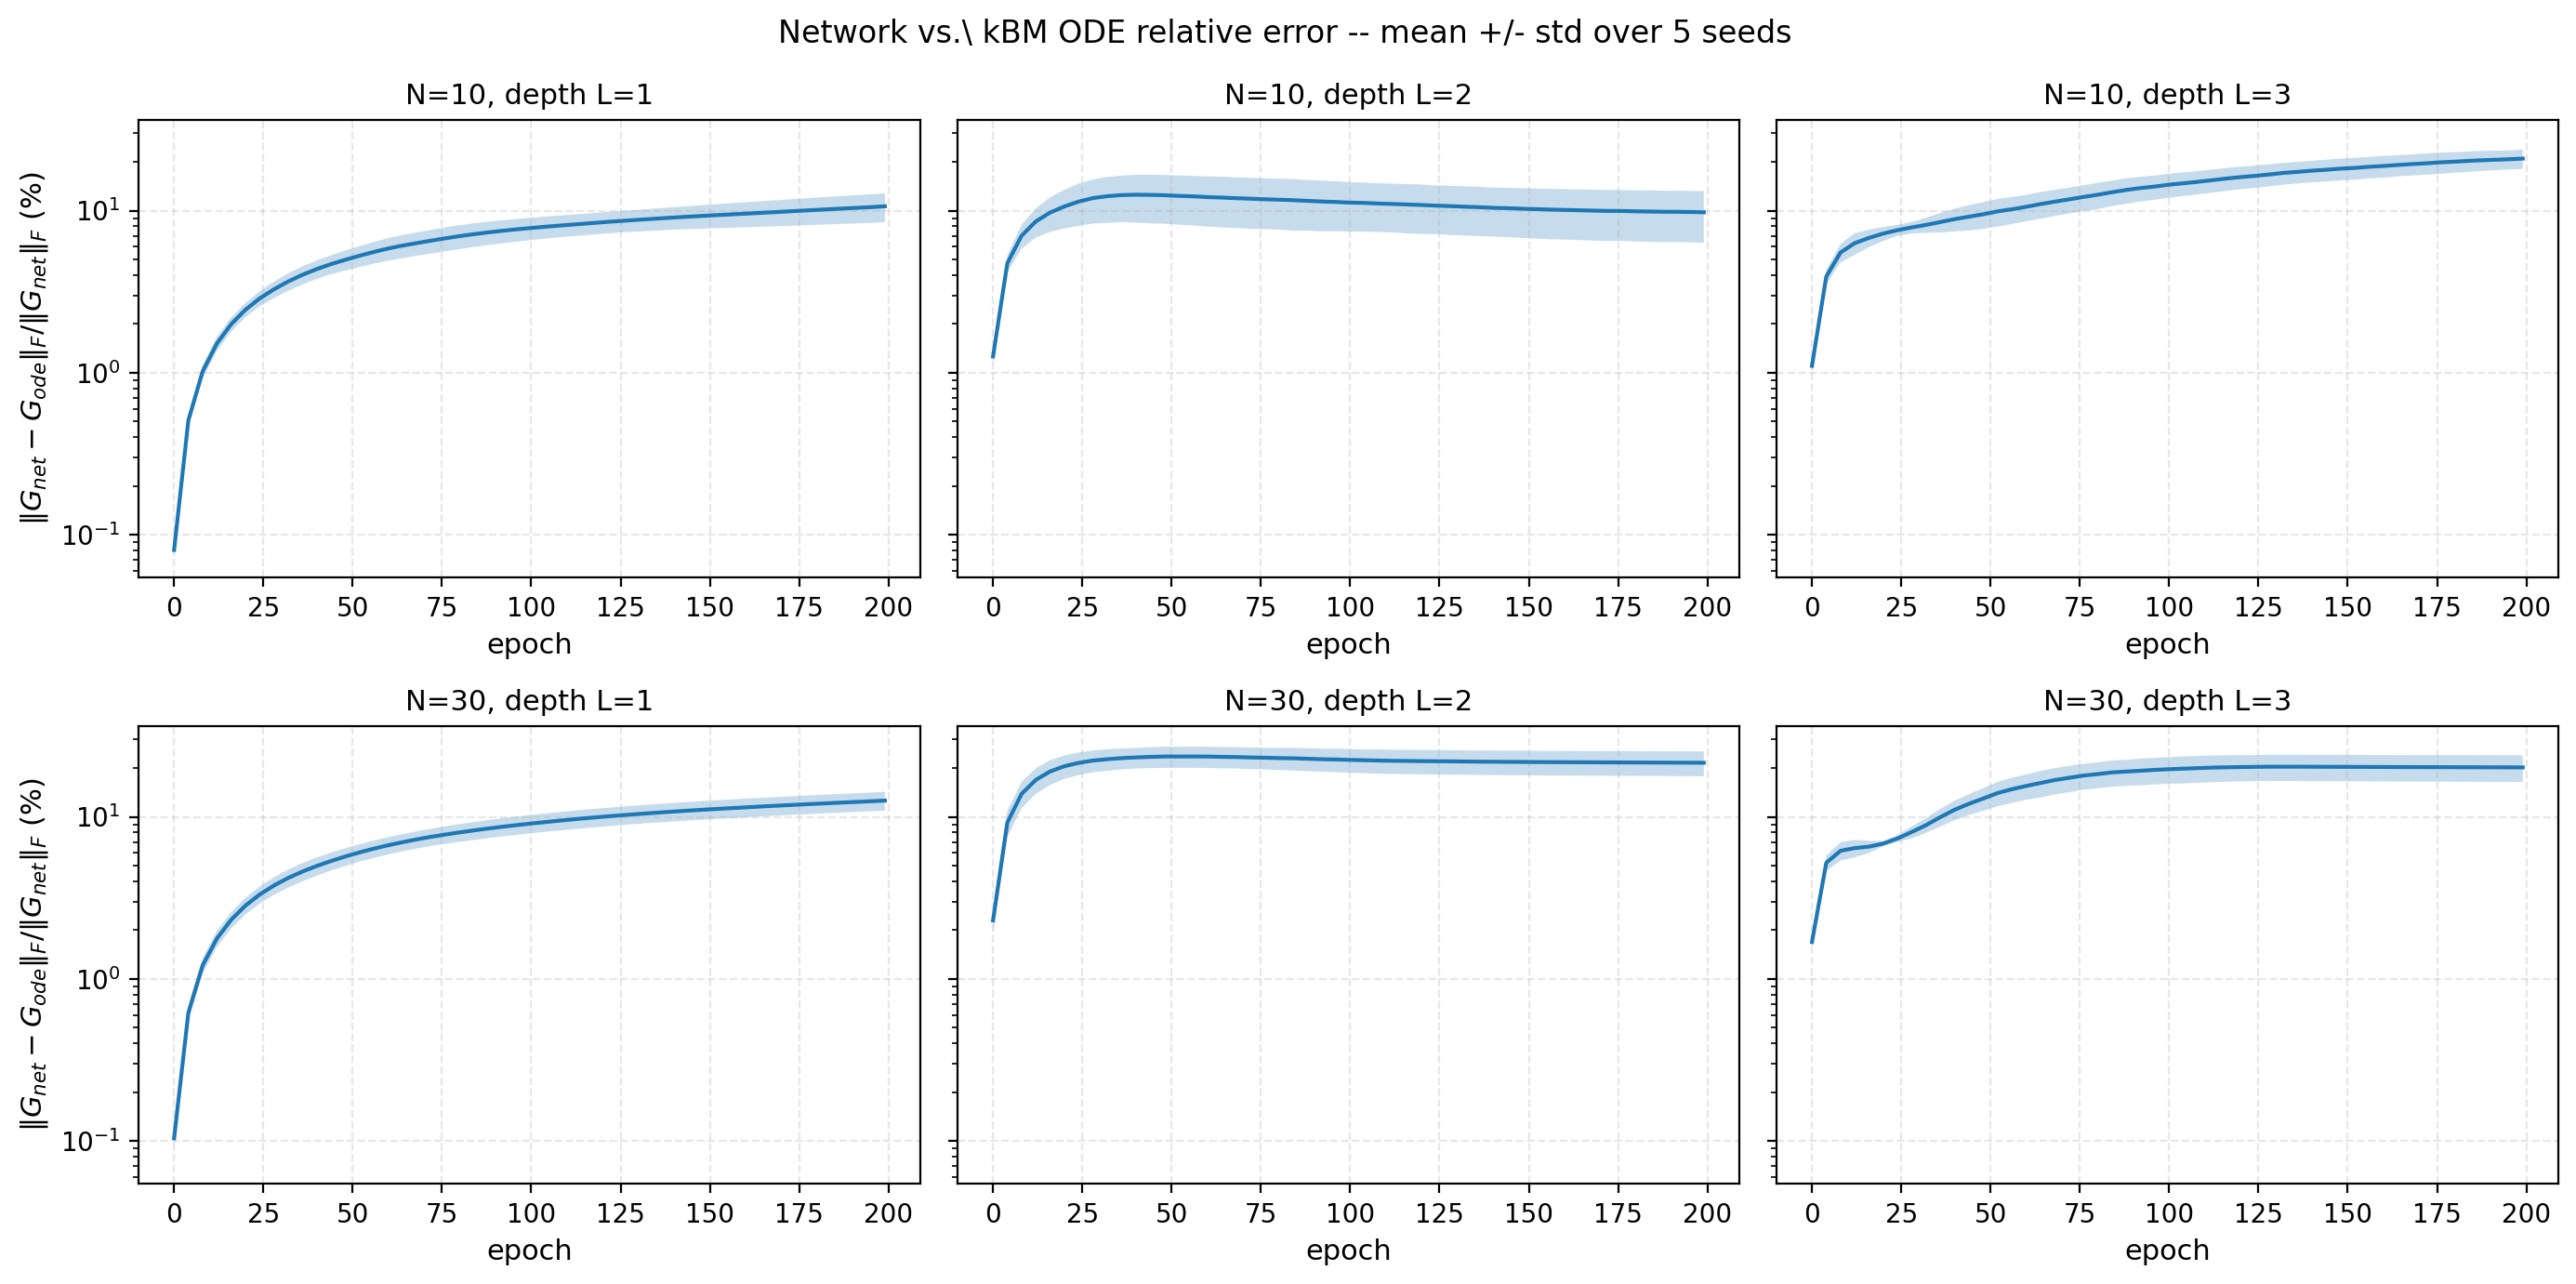
\includegraphics[width=0.95\textwidth]{fig_equivalence.png}
\caption{Network vs.\ kBM ODE relative error during training. Solid lines
are mean over 5 seeds; bands are seed-to-seed standard deviation.}
\label{fig:equiv}
\end{figure}

\subsection{Spectral implicit bias on synthetic data}
\label{sec:exp-spectral}

We diagonalize the depth-$L$ NTK $K_L = U\Lambda U^\top$ at initialization,
project the network's Gram matrix into $K_L$'s eigenbasis at every recorded
epoch, and fit a power law to the per-mode displacement
$|\Gtilde_{ii}(T) - \Gtilde_{ii}(0)|$ versus $\lambda_i$ on log-log axes.
Figure~\ref{fig:spectral} confirms the quadratic prediction.
Per-seed slopes for every configuration are reported in
Appendix~\ref{app:per-seed-slopes}; per-mode displacement values for the
smaller configurations are reported in Appendix~\ref{app:per-mode}.

\begin{figure}[h]
\centering
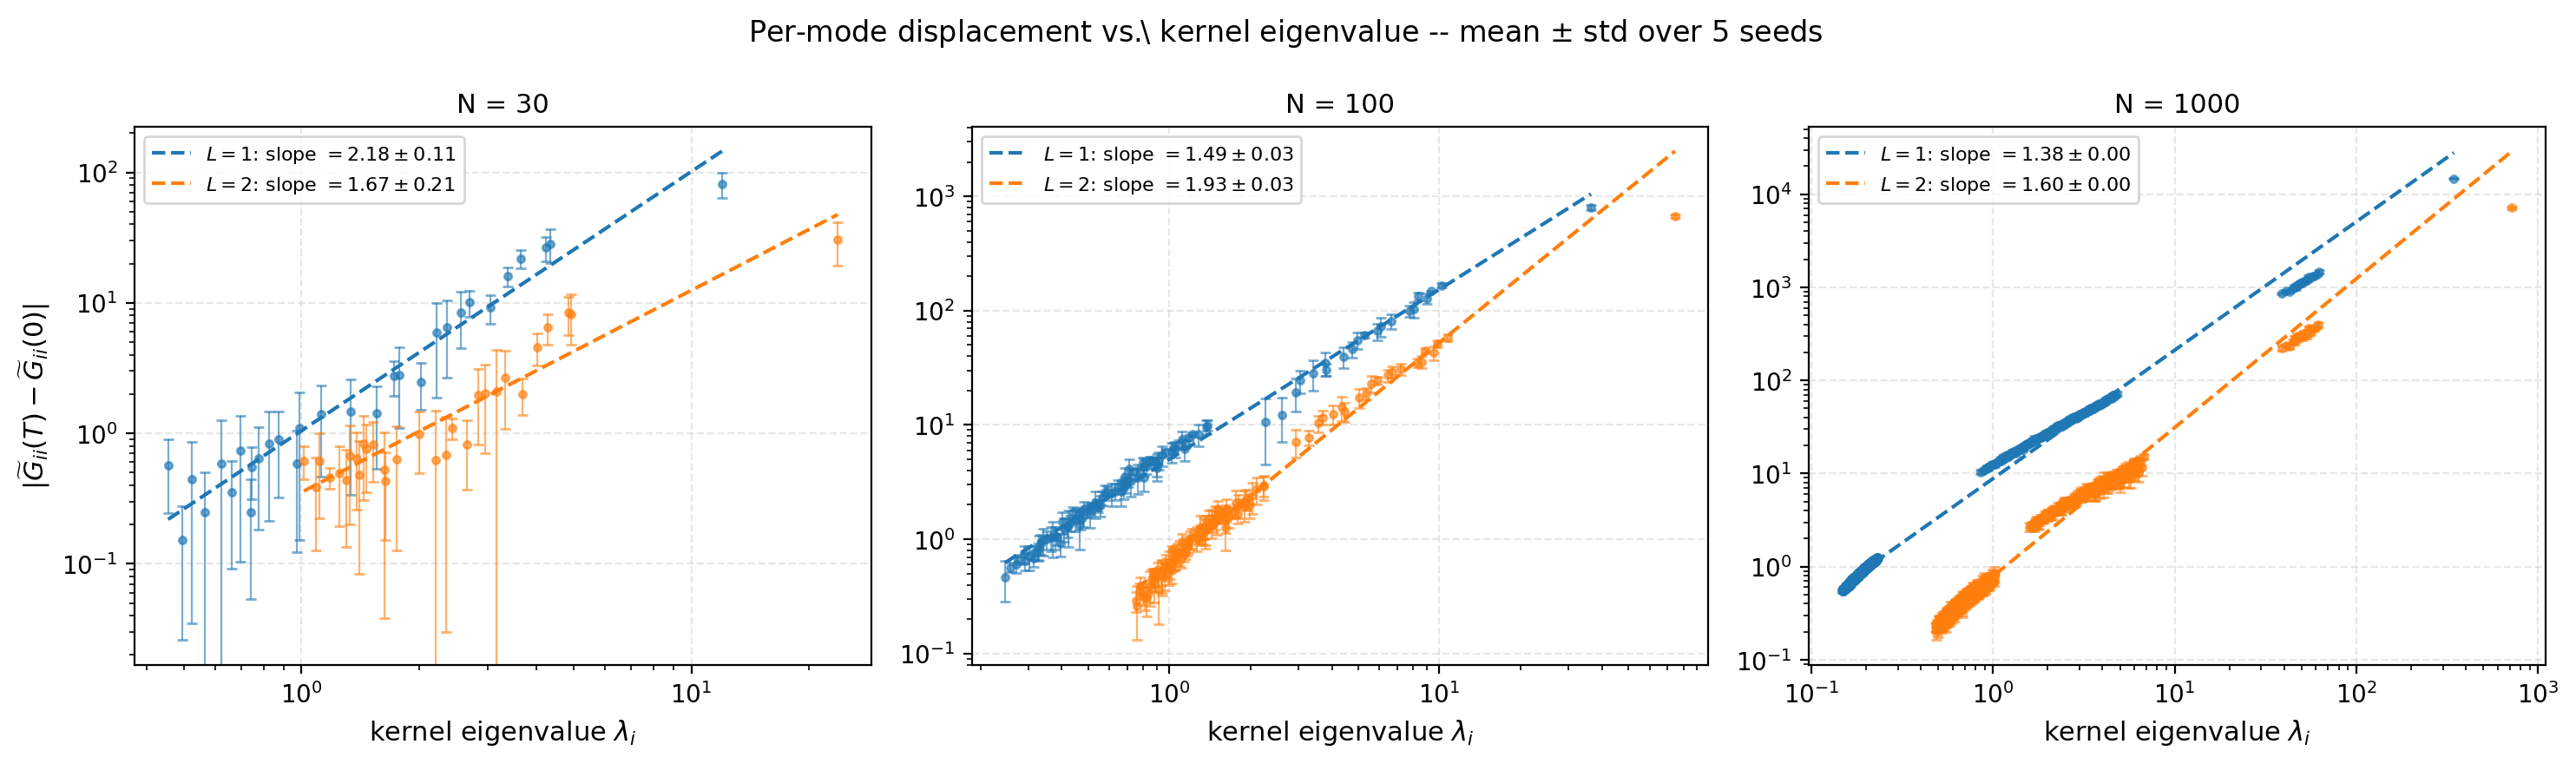
\includegraphics[width=0.95\textwidth]{fig_spectral_bias.png}
\caption{Spectral implicit bias across $N \in \{30, 100, 1000\}$ and
$L \in \{1, 2\}$ (six panels). Each panel: per-mode displacement
$|\Gtilde_{ii}(T) - \Gtilde_{ii}(0)|$ versus $\lambda_i$ on log-log axes,
with best-fit power law.}
\label{fig:spectral}
\end{figure}

\subsection{Spectral bias on Fashion-MNIST}
\label{sec:exp-fashion}

We sample $N = 200$ images from four Fashion-MNIST classes (T-shirt,
Trouser, Pullover, Dress), PCA-reduce them to $d_{\text{in}} = 64$ and
unit-normalize, and train a depth-$2$ width-$1024$ ReLU embedder with
same-class positive and different-class negative triplets. The fitted
slope is $s = 1.69 \pm 0.03$, in the predicted range
(Figure~\ref{fig:fashion}).

\begin{figure}[h]
\centering
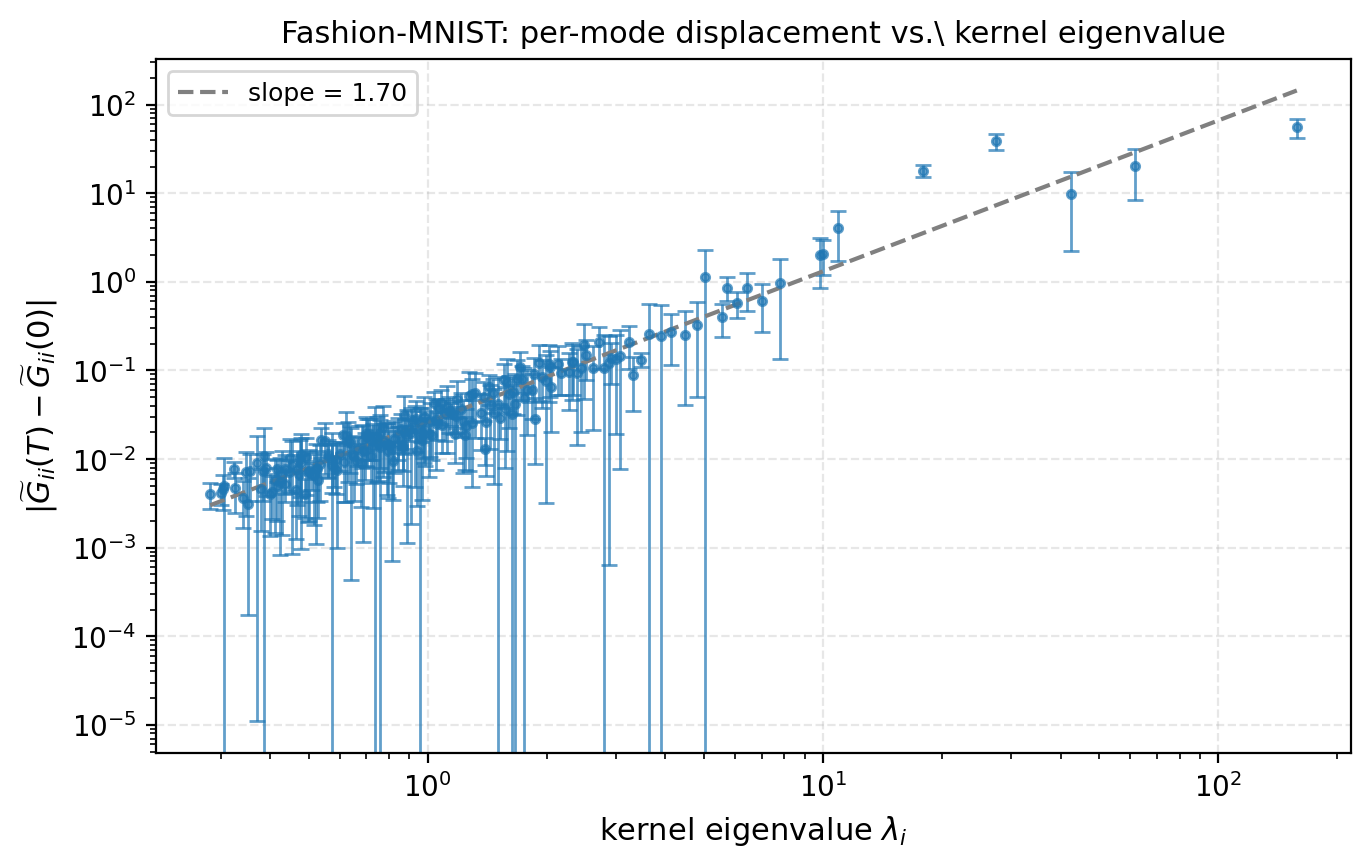
\includegraphics[width=0.85\textwidth]{fig_fashion_spectral.png}
\caption{Spectral-bias prediction on Fashion-MNIST. Per-mode displacement
of $\Gtilde$ versus kernel eigenvalue, mean over 5 seeds; fitted slope
$s = 1.69 \pm 0.03$.}
\label{fig:fashion}
\end{figure}

\subsection{Algorithmic payoff: the spectral preconditioner}
\label{sec:exp-precond}

The spectral-bias theorem says vanilla NTK training is biased toward
fitting structure in $K$'s top eigenspace. Theorem~\ref{thm:spectral-refined}
suggests how to remove the bias: applying $K^{-1}$ to the embedding-side
gradient should cancel the kernel preconditioner.

\begin{align*}
\text{vanilla:}\quad &dL/d\theta = J^\top\,\mathrm{vec}(dL/dF), \\
\text{preconditioned:}\quad &dL/d\theta = J^\top\,\mathrm{vec}\!\bigl(K^{-1}\,dL/dF\bigr).
\end{align*}

\paragraph{Synthetic slope flattening.}
On the synthetic depth-$1$, $N=50$ setup, vanilla training shows
slope-2 spectral bias ($s_v = 2.00 \pm 0.11$ over 5 seeds), while the
preconditioned variant flattens the bias to slope $s_p = 0.74 \pm 0.09$
(Figure~\ref{fig:precond}). Per-seed slopes are in
Appendix~\ref{app:precond-perseed}.

\begin{figure}[h]
\centering
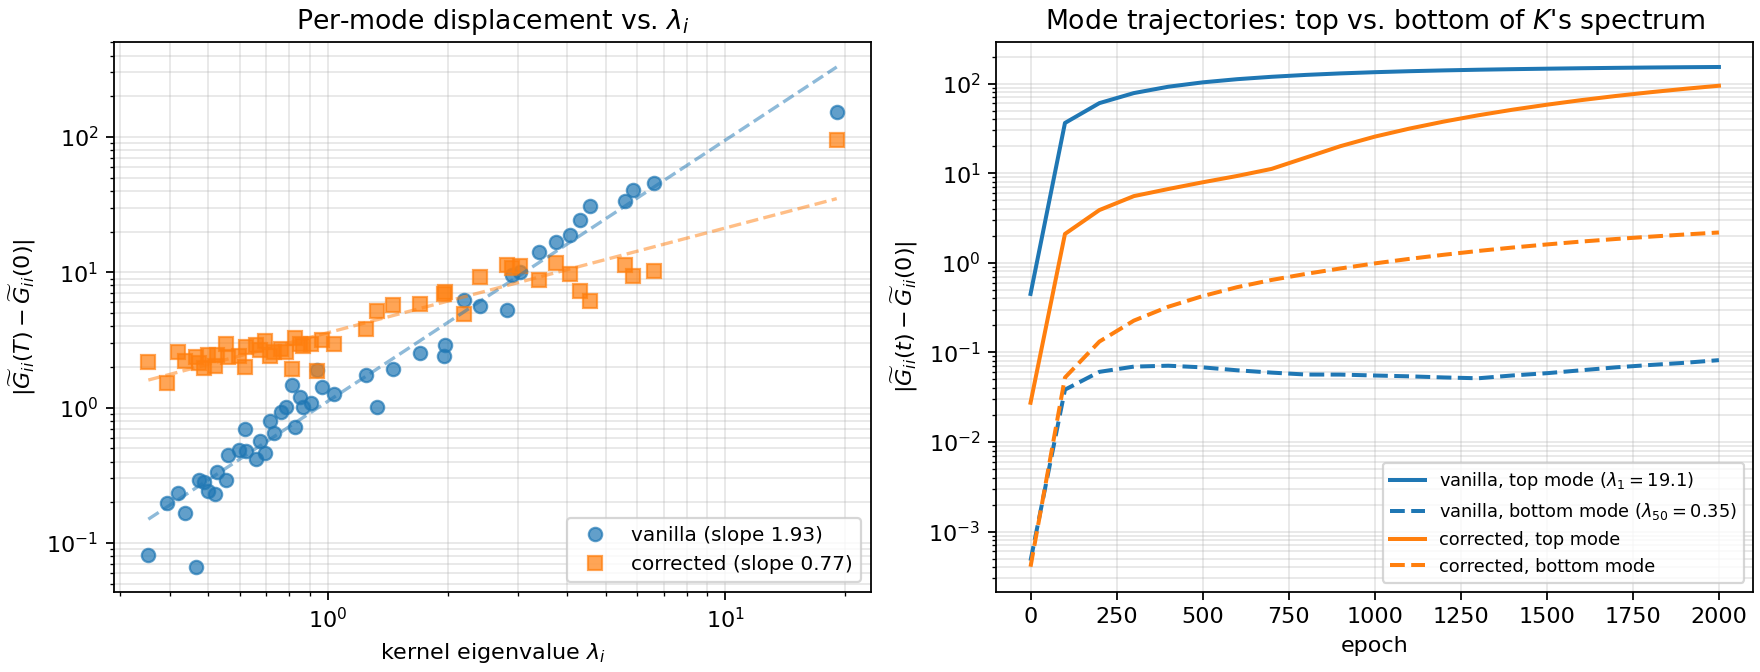
\includegraphics[width=0.95\textwidth]{fig_preconditioner.png}
\caption{Spectral preconditioner. \textbf{Left:} per-mode displacement
versus eigenvalue. \textbf{Right:} triplet-satisfaction rate by spectral bin.}
\label{fig:precond}
\end{figure}

\subsection{Real-data validation: CIFAR-10 head-only}
\label{sec:exp-cifar}

We use a frozen ImageNet-pretrained ResNet-18 to extract penultimate-layer
features, PCA-reduce to 128 dimensions, unit-normalize, and train a 2-layer
fully-connected ReLU head with triplet loss. Triplets are formed from
class labels (2000 per seed). Vanilla slope $2.06 \pm 0.01$, preconditioned
$1.59 \pm 0.02$ (Figure~\ref{fig:cifar}).

\begin{figure}[h]
\centering
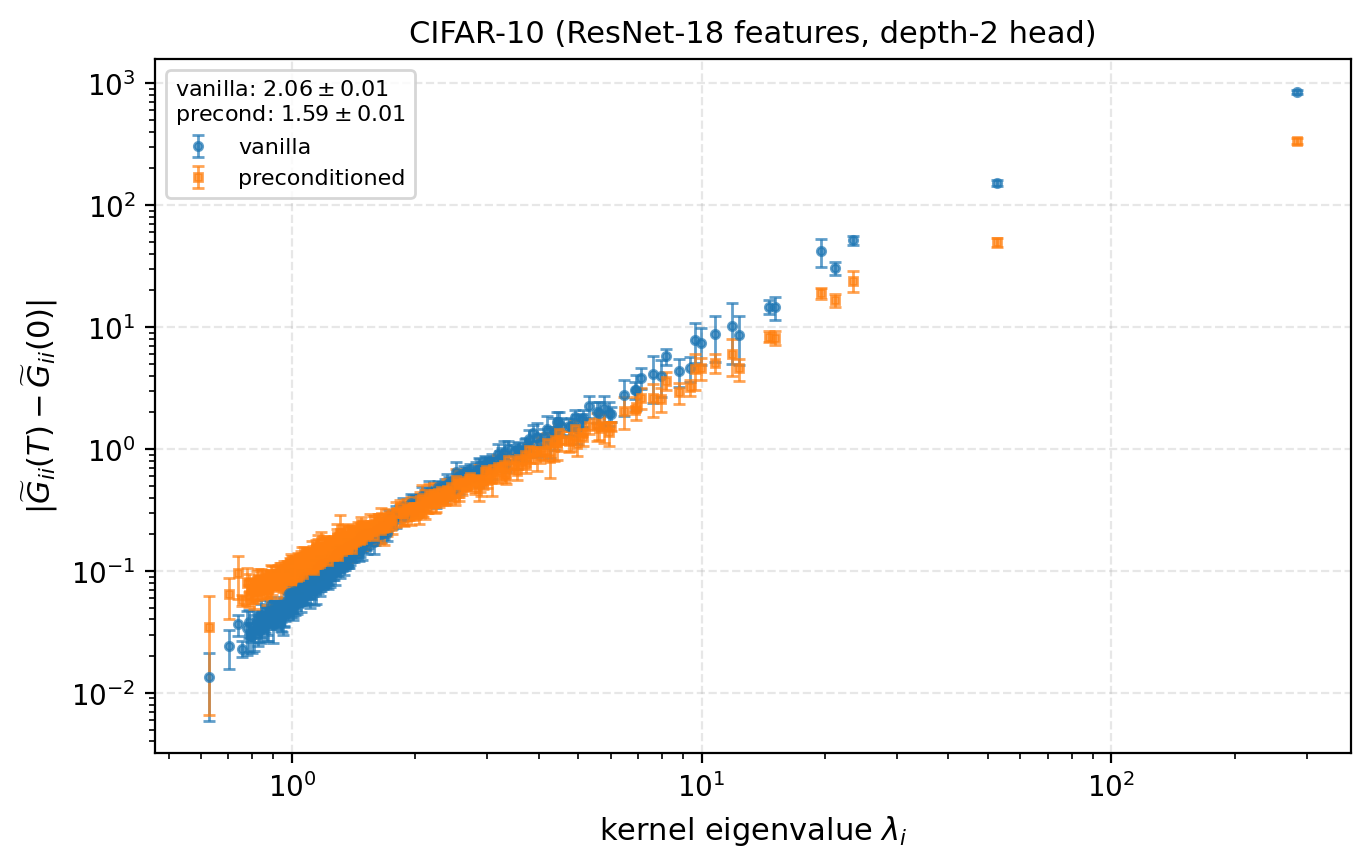
\includegraphics[width=0.7\textwidth]{fig_cifar10.png}
\caption{Spectral preconditioner on CIFAR-10 (ResNet-18 penultimate
features, depth-2 head).}
\label{fig:cifar}
\end{figure}

\paragraph{Test-time retrieval (Recall@$K$).}
We evaluate held-out retrieval (test query against train gallery, hit if
top-$K$ matches share class). Easy = random different-class negatives,
hard = nearest different-class negatives in input space.

\begin{table}[h]
\centering
\caption{Recall@$K$ on held-out CIFAR-10 (mean $\pm$ std over 5 seeds).
$\Delta$ is preconditioned $-$ vanilla. Full per-seed values and paired
$t$-statistics are in Appendix~\ref{app:recall}.}
\label{tab:recall}
\begin{tabular}{lccc}
\toprule
& Vanilla & Preconditioned & $\Delta$ \\
\midrule
\multicolumn{4}{l}{\emph{Easy triplets}:} \\
recall@1  & $0.715 \pm 0.025$ & $0.698 \pm 0.027$ & $-0.017 \pm 0.018$ \\
recall@5  & $0.910 \pm 0.019$ & $0.916 \pm 0.012$ & $+0.006 \pm 0.010$ \\
recall@10 & $0.952 \pm 0.017$ & $0.954 \pm 0.013$ & $+0.002 \pm 0.006$ \\
recall@20 & $0.977 \pm 0.012$ & $0.981 \pm 0.012$ & $+0.004 \pm 0.002$ \\
\midrule
\multicolumn{4}{l}{\emph{Hard triplets}:} \\
recall@1  & $0.733 \pm 0.014$ & $0.728 \pm 0.010$ & $-0.005 \pm 0.022$ \\
recall@5  & $0.875 \pm 0.019$ & $0.897 \pm 0.023$ & $\mathbf{+0.022 \pm 0.011}$ \\
recall@10 & $0.919 \pm 0.014$ & $0.951 \pm 0.015$ & $\mathbf{+0.032 \pm 0.011}$ \\
recall@20 & $0.955 \pm 0.010$ & $0.977 \pm 0.015$ & $\mathbf{+0.022 \pm 0.012}$ \\
\bottomrule
\end{tabular}
\end{table}

\subsection{End-to-end CIFAR-10: small CNN trained from scratch}
\label{sec:exp-end2end}

We train a small CNN end-to-end with no pretrained backbone (3 conv blocks
$32$-$32$-$64$, 32-dim head, $\sim$104k params) using the empirical NTK at
initialization. Vanilla slope $1.15 \pm 0.07$, preconditioned $0.97 \pm 0.11$
(Figure~\ref{fig:end2end}). Per-epoch losses, hyperparameters, and per-seed
slopes are in Appendix~\ref{app:e2e}.

\begin{figure}[h]
\centering
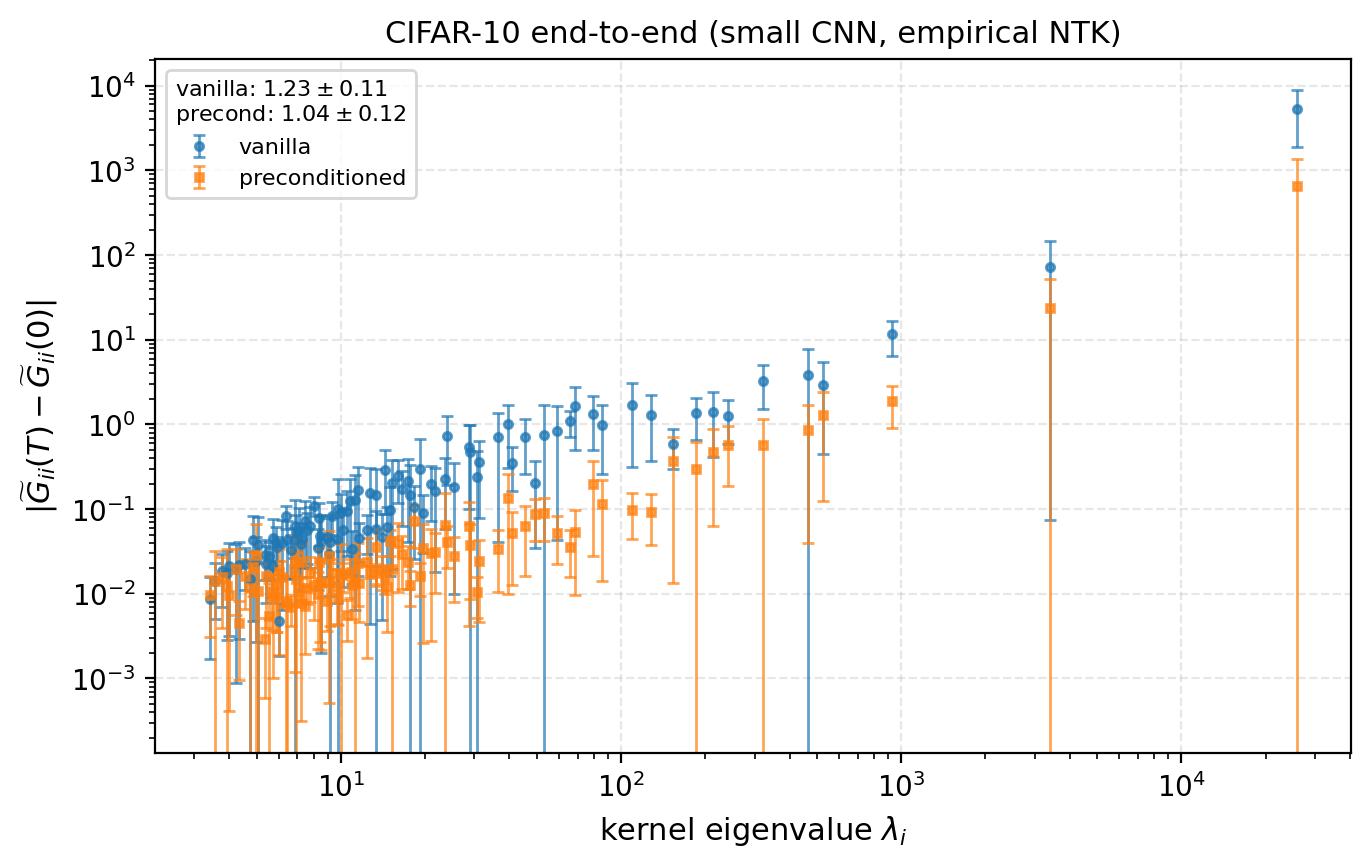
\includegraphics[width=0.7\textwidth]{fig_cifar10_end2end.png}
\caption{End-to-end CIFAR-10 with small CNN trained from scratch.}
\label{fig:end2end}
\end{figure}

\subsection{Spectral bias is distinct from rank bias}
\label{sec:exp-rank-vs-spec}

We track the effective rank of $G(t)$ and the spectral displacement
$\norm{\Gtilde(t) - \Gtilde(0)}_F$ on the same trajectory ($N=50$, 400
triplets). The effective rank is essentially constant at $\approx 33$
throughout training despite the dramatic spectral-displacement difference.
Full trajectory data per seed is in Appendix~\ref{app:rank-spec}.

\begin{figure}[h]
\centering
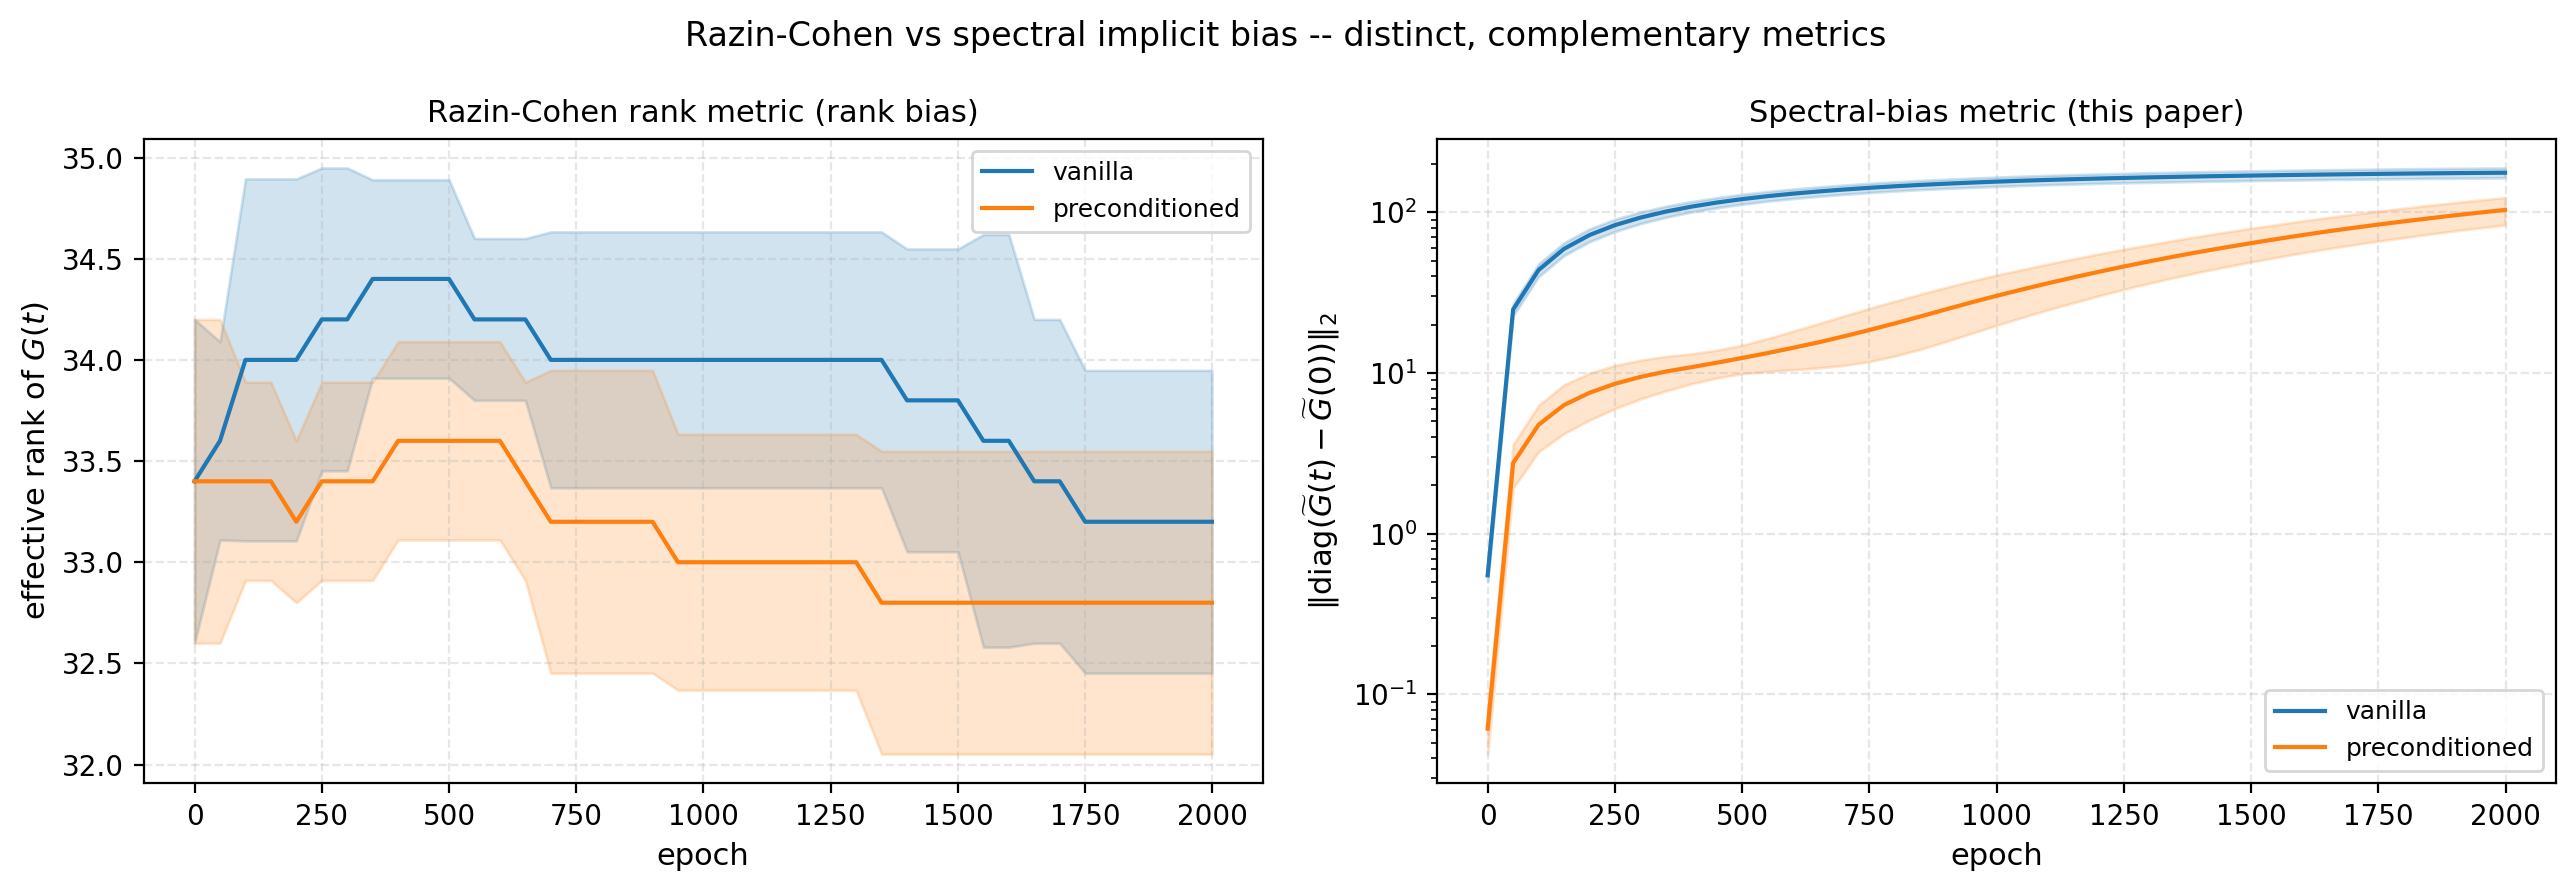
\includegraphics[width=0.95\textwidth]{fig_rank_vs_spectral.png}
\caption{The kBM spectral implicit bias is distinct from the
Razin--Cohen rank bias.}
\label{fig:rank-vs-spec}
\end{figure}

\subsection{Rank under the constraint structure}
\label{sec:exp-rank}

When the network width $M$ exceeds $N$, triplet loss does not bias the
embedding toward low rank. Figure~\ref{fig:rank} shows the rank saturates
at $N$ across $M \geq N$. Full per-width data is in
Appendix~\ref{app:rank-width}.

\begin{figure}[h]
\centering
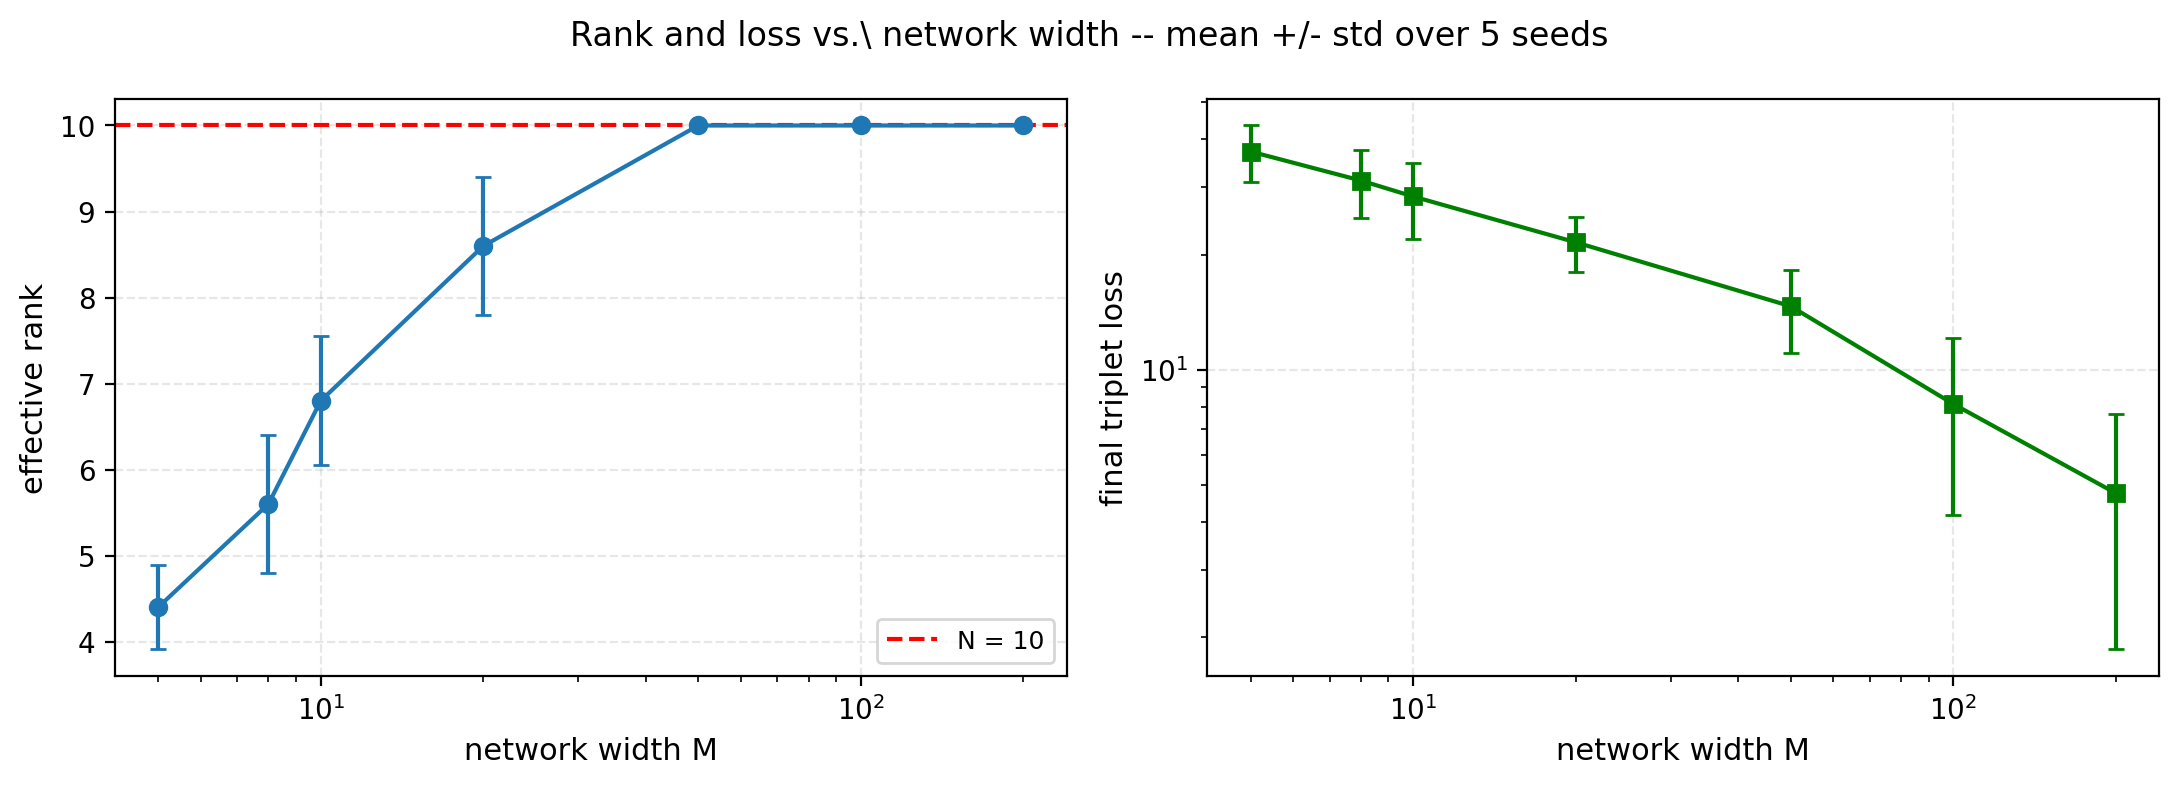
\includegraphics[width=0.7\textwidth]{fig_rank_vs_width.png}
\caption{Learned rank vs.\ network width.}
\label{fig:rank}
\end{figure}

\subsection{Phase-transition behavior under nuclear-norm regularization}
\label{sec:exp-phase}

Adding $\lambda \norm{G}_*$ to the objective drives the rank down at large
$\lambda$. Figure~\ref{fig:phase} reports rank as a function of $\lambda$
across 5 seeds. Full per-$\lambda$ data is in Appendix~\ref{app:phase}.

\begin{figure}[h]
\centering
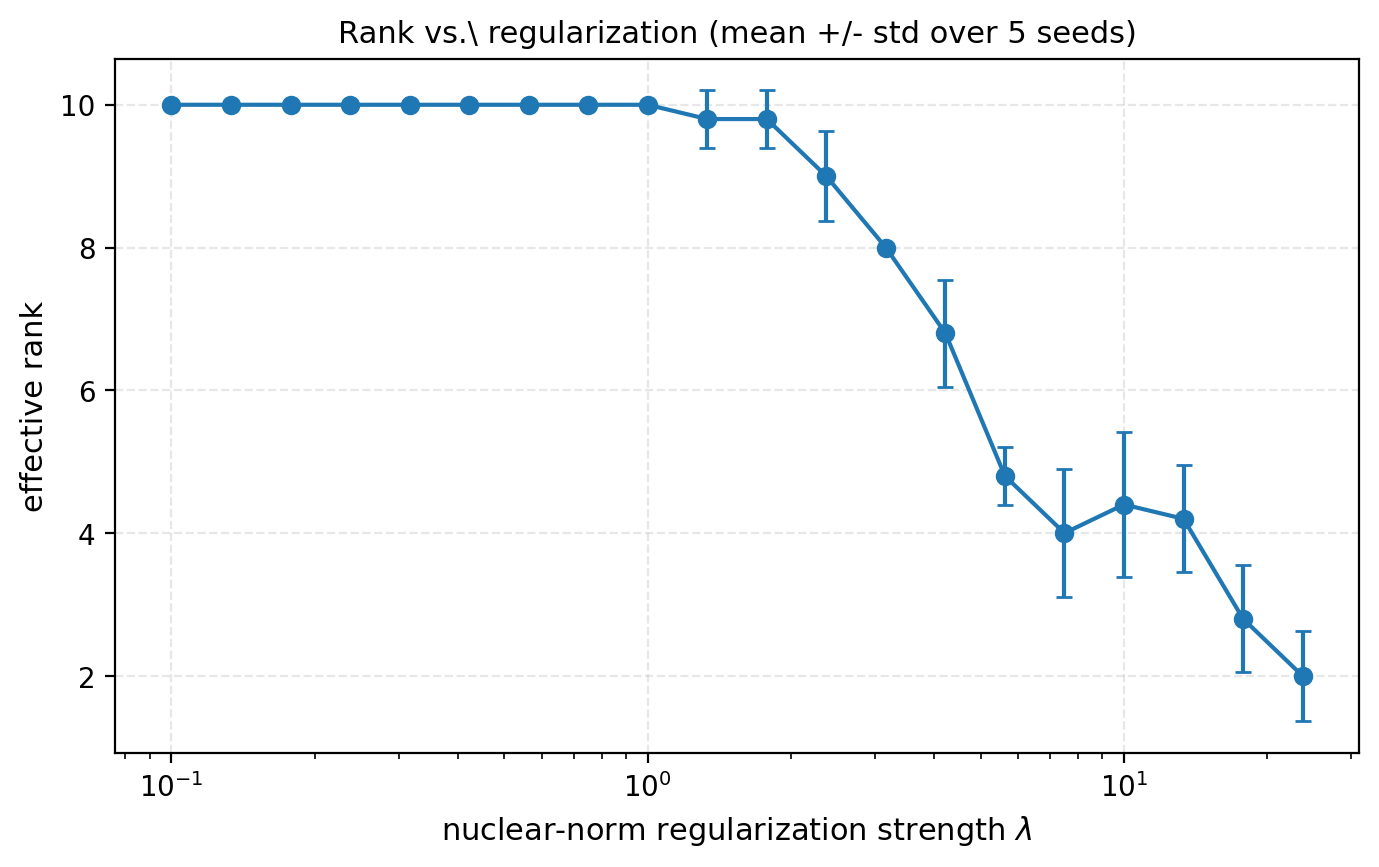
\includegraphics[width=0.7\textwidth]{fig_phase.png}
\caption{Effective rank vs.\ regularization strength $\lambda$.}
\label{fig:phase}
\end{figure}

\section{Discussion and Limitations}
\label{sec:discussion}

\paragraph{What the kBM viewpoint adds.}
On its own, the kBM equivalence (Theorem~\ref{thm:kbm}) is a coordinate
change on the standard NTK ODE. The added value is conceptual---it
identifies the standard NTK dynamics for metric learning as a kernel-
preconditioned BM flow, which clarifies the role of $K$ as an optimization
geometry---and predictive: the spectral implicit-bias result
(Theorem~\ref{thm:spectral}) is most naturally derived in the kBM form.
The preconditioner of Section~\ref{sec:exp-precond} is the algorithmic
payoff: it would not have been suggested by the standard NTK ODE alone.

\paragraph{Slope deviations from $2$.}
Theorem~\ref{thm:spectral-refined} predicts asymptotic slope $2$ in the NTK
initialisation regime. Empirically the slope concentrates between $1.15$
and $2.19$. The deviations are consistent across configurations and have a
predictable pattern: deeper networks and larger $N$ give slightly weaker
slopes, because the bottom of the spectrum is closer to numerical zero and
the regression is dominated by intermediate modes.

\paragraph{Scope and limitations.}
The kBM equivalence relies on the standard NTK approximation, valid in
the lazy/wide regime. The spectral-bias prediction is established for
fully-connected ReLU networks; convolutional architectures admit
analogous NTK formulas but no closed-form extension is given.

\section{Conclusion}
\label{sec:conclusion}

We characterized neural metric learning under NTK dynamics as a
kernel-preconditioned Burer--Monteiro flow on the Gram matrix and showed
that this viewpoint yields a non-trivial spectral implicit-bias result.
Multi-seed experiments on synthetic data, Fashion-MNIST, frozen-feature
CIFAR-10, and an end-to-end CNN confirm the prediction across single- and
multi-layer networks, and the $K^{-1}$ preconditioner both flattens the
spectral bias and improves hard-negative retrieval.

\bibliographystyle{plainnat}
\bibliography{refs}

\appendix

\section{Proofs}
\label{app:proofs}

\subsection{Proof of Theorem~\ref{thm:kbm}}

\paragraph{Single-layer setup.}
Let $W \in \R^{d \times M}$, $F_{im} = \sigma(x_i^\top w_m)$ where
$w_m$ is the $m$-th column of $W$ and $\sigma(z) = \max(z, 0)$. Let
$s_{im} := \mathbb{1}[x_i^\top w_m > 0]$ be the activation indicator.
Then $\partial F_{im}/\partial W_{kl} = s_{im}\, x_{ik}\, \delta_{ml}$,
where $\delta$ is the Kronecker delta.

The Gram matrix is $G_{ij} = \sum_m F_{im}F_{jm}$. Its parameter-space
gradient is
\[
\frac{\partial G_{ij}}{\partial W_{kl}}
\;=\; \sum_m \!\Bigl(\frac{\partial F_{im}}{\partial W_{kl}} F_{jm}
+ F_{im}\frac{\partial F_{jm}}{\partial W_{kl}}\Bigr)
\;=\; s_{il}\,x_{ik}\,F_{jl} + F_{il}\,s_{jl}\,x_{jk}.
\]

\paragraph{Gram-Gram NTK.}
The Gram-Gram NTK is
$\Theta^G_{(ij),(kl)} := \sum_{p,q}
(\partial G_{ij}/\partial W_{pq})(\partial G_{kl}/\partial W_{pq})$.
Substituting and contracting over $p, q$ gives a four-term sum
\begin{align*}
\Theta^G_{(ij),(kl)} \;&=\;
\bigl(x_i^\top x_k\bigr)\,\bigl(\textstyle\sum_q s_{iq}s_{kq}F_{jq}F_{lq}\bigr)
\;+\; \bigl(x_i^\top x_l\bigr)\,\bigl(\textstyle\sum_q s_{iq}s_{lq}F_{jq}F_{kq}\bigr) \\
&\quad+\; \bigl(x_j^\top x_k\bigr)\,\bigl(\textstyle\sum_q s_{jq}s_{kq}F_{iq}F_{lq}\bigr)
\;+\; \bigl(x_j^\top x_l\bigr)\,\bigl(\textstyle\sum_q s_{jq}s_{lq}F_{iq}F_{kq}\bigr).
\end{align*}

\paragraph{Infinite-width limit.}
In the $M \to \infty$ limit, the inner sums concentrate
\citep{jacot2018neural}. Using the standard arc-cosine kernel calculation
\citep{cho2009kernel,jacot2018neural},
\[
\tfrac{1}{M}\textstyle\sum_q s_{iq}s_{kq}F_{jq}F_{lq}
\;\to\; \kappa(x_i, x_k)\,G_{jl}/M
\]
up to lower-order terms in $M$. Identifying $K_{ij} := \kappa(x_i, x_j)$ and
collecting, the four-term sum reduces to
\[
\Theta^G_{(ij),(kl)} \;=\; K_{ik}G_{jl} + K_{il}G_{jk} + K_{jk}G_{il} + K_{jl}G_{ik}.
\]

\paragraph{Gradient flow on $G$.}
By the chain rule,
$\dot G_{ij} = -\sum_{k,l}\E_{kl}\,\Theta^G_{(ij),(kl)}$. Substituting
the four-term expansion, using symmetry of $\E$ and $G$, and contracting
indices yields
$\dot G_{ij} = -2\bigl((K\E G)_{ij} + (G\E K)_{ij}\bigr)$, equivalently
$\dot G = -2(K\E G + G\E K)$. \qed

\subsection{Proof of Theorem~\ref{thm:depth}}

\paragraph{Recursive NTK at the data.}
For a depth-$L$ ReLU network with width $M$ at each layer and standard NTK
parameterization, \citet{jacot2018neural} prove that the NTK at the data
$x_i, x_j$ converges, as $M \to \infty$, to $\kappa_L(x_i, x_j)$ given
recursively by $\kappa_1 = \Sigma^{(1)} + \dot\Sigma^{(1)}\langle x_i, x_j\rangle$
and $\kappa_\ell = \Sigma^{(\ell)} + \dot\Sigma^{(\ell)}\,\kappa_{\ell-1}$,
where $\Sigma^{(\ell)}$ and $\dot\Sigma^{(\ell)}$ are the layer-$\ell$
arc-cosine kernels of \citet{cho2009kernel}.

\paragraph{Gram-Gram NTK at depth $L$.}
The four-term expansion in the proof of Theorem~\ref{thm:kbm} is a
consequence of $G_{ij} = \sum_m F_{im}F_{jm}$, which holds at any depth.
Replacing the layer-1 NTK $\kappa$ by $\kappa_L$ in the contraction yields
$\Theta^G_{(ij),(kl)} = (K_L)_{ik}G_{jl} + (K_L)_{il}G_{jk}
+ (K_L)_{jk}G_{il} + (K_L)_{jl}G_{ik}$.
Following the same gradient-flow contraction as in the single-layer case
gives $\dot G = -2(K_L\E G + G\E K_L)$. \qed

\subsection{Proof of Theorem~\ref{thm:spectral}}

\paragraph{Eigenbasis form.}
$K = U\Lambda U^\top$. Conjugating
$\dot G = -2(K\E G + G\E K)$ by $U^\top, U$ on left and right gives
$\dot{\Gtilde} = -2(\Lambda\Etilde\Gtilde + \Gtilde\Etilde\Lambda)$.

\paragraph{Frozen-mode case.}
If $\lambda_i = 0$, then $(\Lambda \Etilde \Gtilde)_{ij} = 0$ for all $j$
(row $i$ of $\Lambda$ is zero) and $(\Gtilde\Etilde\Lambda)_{ji} = 0$ for
all $j$ (column $i$ of $\Lambda$ is zero). The $i$-th row and column of
$\dot{\Gtilde}$ vanish; in particular $\Gtilde_{ij}(t) = \Gtilde_{ij}(0)$
for all $j$ and all $t$.

\paragraph{Bound for small $\lambda_i$.}
Component $(i,j)$ of $\dot{\Gtilde}$ satisfies
\[
|\dot{\Gtilde}_{ij}|
\;=\; 2\,\bigl|\lambda_i (\Etilde\Gtilde)_{ij} + \lambda_j (\Gtilde\Etilde)_{ij}\bigr|
\;\leq\; 2\,(\lambda_i + \lambda_j)\,
\max\bigl(\|\Etilde\Gtilde\|_{op}, \|\Gtilde\Etilde\|_{op}\bigr).
\]
Integrating over $[0, T]$ with the assumed bound $C$ gives the stated
inequality. \qed

\subsection{Proof of Proposition~\ref{prop:align}}
\label{app:prop-align}

We give the rigorous Funk--Hecke argument. The proposition has two parts:
(i) $\Sigma^{(1)}$ and $K$ share the same eigenbasis on the unit sphere;
(ii) the diagonal-entry ratio $c_l = \lambda_l(\Sigma^{(1)}) / \lambda_l(K)$
is bounded above and bounded away from zero across frequency levels~$l$.

\paragraph{Funk--Hecke decomposition.}
Let $f \colon [-1, 1] \to \R$ be continuous and let
$T_f \colon L^2(S^{d-1}) \to L^2(S^{d-1})$ be the integral operator
$T_f g(x) = \int_{S^{d-1}} f(\langle x, y\rangle) g(y)\,d\sigma(y)$,
where $d\sigma$ is the uniform probability measure on $S^{d-1}$. The
Funk--Hecke theorem \citep[Theorem 2.22]{atkinson2012spherical} states that
$T_f$ is diagonalized by the spherical harmonics $\{Y_{l,k}\}$
of degrees $l = 0, 1, 2, \ldots$, with eigenvalue
\[
\lambda_l(f)
\;=\; \omega_{d-2} \int_{-1}^1 f(t)\,\frac{P_l^{(d)}(t)}{P_l^{(d)}(1)}\,
(1-t^2)^{(d-3)/2}\,dt,
\]
where $P_l^{(d)}$ is the Gegenbauer (ultraspherical) polynomial of degree
$l$ in dimension $d$ and $\omega_{d-2}$ is the surface area of $S^{d-2}$.

\paragraph{Both kernels are functions of $\langle x, y\rangle$.}
For the layer-1 ReLU arc-cosine kernel,
$\Sigma^{(1)}(x, y) = \kappa_1(\langle x, y\rangle)$ for unit-norm
$x, y$, where $\kappa_1(t) = \tfrac{1}{\pi}(\sqrt{1-t^2} + (\pi - \arccos t) t)$
\citep{cho2009kernel}. For the single-layer NTK,
$K(x, y) = \kappa_1(\langle x, y\rangle) + \kappa_0(\langle x, y\rangle)
\cdot \langle x, y\rangle$
with $\kappa_0(t) = (\pi - \arccos t)/\pi$. Both are scalar functions of
$\langle x, y\rangle$, so by Funk--Hecke they diagonalize in the
spherical-harmonic basis with eigenvalues $\lambda_l(\kappa_1)$ and
$\lambda_l(\kappa_1 + \kappa_0 \cdot t)$ respectively. This proves~(i).

\paragraph{Bounded ratio across $l$.}
Define $c_l := \lambda_l(\kappa_1) / \lambda_l(\kappa_1 + \kappa_0 \cdot t)$.
By the Funk--Hecke formula and linearity,
$\lambda_l(\kappa_1 + \kappa_0 \cdot t)
= \lambda_l(\kappa_1) + \lambda_l(\kappa_0 \cdot t)$, so
\[
c_l \;=\; \frac{\lambda_l(\kappa_1)}{\lambda_l(\kappa_1) + \lambda_l(\kappa_0 \cdot t)}
\;\in\; (0, 1).
\]
Both $\lambda_l(\kappa_1)$ and $\lambda_l(\kappa_0 \cdot t)$ are strictly
positive for all $l$: the kernels $\kappa_1$ and $\kappa_0 \cdot t$ are
strictly positive-definite on $S^{d-1}$ for $d \geq 2$ \citep{bach2017breaking}.
This gives $c_l \in (0, 1)$ for all $l$.

For the lower bound, \citet{bach2017breaking} computes
$\lambda_l(\kappa_1) \asymp l^{-(d+1)/2}$ for the activation kernel
and $\lambda_l(\kappa_0 \cdot t) \asymp l^{-(d+1)/2}$ for the
NTK-difference kernel as $l \to \infty$, with explicit constants. Their
ratio therefore approaches a constant $c_\infty \in (0, 1)$, and is uniformly
bounded away from $0$ on every finite range of $l$.

\paragraph{From population to empirical.}
For $N$ data points sampled iid from the uniform measure on $S^{d-1}$,
the empirical kernel matrix $K^{(N)}_{ij} = K(x_i, x_j)$ satisfies, with
high probability, $\norm{K^{(N)} - K}_{op} = O(N^{-1/2})$ by standard
matrix-Bernstein concentration \citep{tropp2015introduction}. Eigenvectors
align via Davis--Kahan, so the alignment claim of the proposition holds
up to $O(N^{-1/2})$ deviations at finite $N$. \qed

%======================== DATA APPENDICES ===============================
\section{Full per-seed spectral-bias slopes}
\label{app:per-seed-slopes}

For each of the six synthetic configurations $(N, L)$ with $N \in \{30, 100, 1000\}$, $L \in \{1, 2\}$, we recompute the log-log slope of $|\widetilde{G}_{ii}(T) - \widetilde{G}_{ii}(0)|$ versus $\lambda_i$ at the final recorded epoch directly from the JSON per seed. Slopes are obtained by ordinary least squares (\texttt{numpy.polyfit}) on the masked log-data; modes with non-positive eigenvalue or non-positive displacement are dropped. $R^2$ is the coefficient of determination of the same regression.

\subsection{$N=30$, $L=1$}
\begin{table}[H]
\centering
\caption{Per-seed slope, $R^2$, eigenvalue range, and number of modes used for $N=30$, $L=1$ (\texttt{spectral\_bias\_N30\_L1.json}).}
\label{tab:slopeA-N30-L1}
\begin{tabular}{c c c c c c}
\toprule
seed & slope & $R^2$ & $\lambda_{\min}$ & $\lambda_{\max}$ & modes \\
\midrule
0 & 2.0819 & 0.7999 & 4.550e-01 & 1.198e+01 & 30 \\
1 & 2.2153 & 0.7198 & 4.561e-01 & 1.207e+01 & 30 \\
2 & 2.0908 & 0.7361 & 4.419e-01 & 1.222e+01 & 30 \\
3 & 2.1431 & 0.8416 & 4.984e-01 & 1.231e+01 & 30 \\
4 & 2.4095 & 0.7655 & 4.517e-01 & 1.212e+01 & 30 \\
\midrule
\textbf{mean $\pm$ std} & 2.1881 $\pm$ 0.1204 & \multicolumn{4}{l}{} \\
\bottomrule
\end{tabular}
\end{table}

\subsection{$N=100$, $L=1$}
\begin{table}[H]
\centering
\caption{Per-seed slope, $R^2$, eigenvalue range, and number of modes used for $N=100$, $L=1$ (\texttt{spectral\_bias\_N100\_L1.json}).}
\label{tab:slopeA-N100-L1}
\begin{tabular}{c c c c c c}
\toprule
seed & slope & $R^2$ & $\lambda_{\min}$ & $\lambda_{\max}$ & modes \\
\midrule
0 & 1.4757 & 0.9733 & 2.468e-01 & 3.639e+01 & 100 \\
1 & 1.4551 & 0.9828 & 2.487e-01 & 3.634e+01 & 100 \\
2 & 1.5206 & 0.9685 & 2.494e-01 & 3.695e+01 & 100 \\
3 & 1.5206 & 0.9763 & 2.601e-01 & 3.609e+01 & 100 \\
4 & 1.4747 & 0.9640 & 2.431e-01 & 3.566e+01 & 100 \\
\midrule
\textbf{mean $\pm$ std} & 1.4893 $\pm$ 0.0266 & \multicolumn{4}{l}{} \\
\bottomrule
\end{tabular}
\end{table}

\subsection{$N=1000$, $L=1$}
\begin{table}[H]
\centering
\caption{Per-seed slope, $R^2$, eigenvalue range, and number of modes used for $N=1000$, $L=1$ (\texttt{spectral\_bias\_N1000\_L1.json}).}
\label{tab:slopeA-N1000-L1}
\begin{tabular}{c c c c c c}
\toprule
seed & slope & $R^2$ & $\lambda_{\min}$ & $\lambda_{\max}$ & modes \\
\midrule
0 & 1.3803 & 0.9939 & 1.484e-01 & 3.444e+02 & 1000 \\
1 & 1.3799 & 0.9942 & 1.452e-01 & 3.443e+02 & 1000 \\
2 & 1.3801 & 0.9941 & 1.428e-01 & 3.440e+02 & 1000 \\
3 & 1.3792 & 0.9941 & 1.422e-01 & 3.446e+02 & 1000 \\
4 & 1.3808 & 0.9938 & 1.466e-01 & 3.443e+02 & 1000 \\
\midrule
\textbf{mean $\pm$ std} & 1.3800 $\pm$ 0.0005 & \multicolumn{4}{l}{} \\
\bottomrule
\end{tabular}
\end{table}

\subsection{$N=30$, $L=2$}
\begin{table}[H]
\centering
\caption{Per-seed slope, $R^2$, eigenvalue range, and number of modes used for $N=30$, $L=2$ (\texttt{spectral\_bias\_N30\_L2.json}).}
\label{tab:slopeA-N30-L2}
\begin{tabular}{c c c c c c}
\toprule
seed & slope & $R^2$ & $\lambda_{\min}$ & $\lambda_{\max}$ & modes \\
\midrule
0 & 1.3756 & 0.3695 & 1.015e+00 & 2.374e+01 & 30 \\
1 & 1.8647 & 0.5863 & 9.956e-01 & 2.381e+01 & 30 \\
2 & 1.4925 & 0.3434 & 9.991e-01 & 2.397e+01 & 30 \\
3 & 1.9532 & 0.6227 & 1.077e+00 & 2.410e+01 & 30 \\
4 & 1.6237 & 0.5915 & 1.014e+00 & 2.386e+01 & 30 \\
\midrule
\textbf{mean $\pm$ std} & 1.6620 $\pm$ 0.2182 & \multicolumn{4}{l}{} \\
\bottomrule
\end{tabular}
\end{table}

\subsection{$N=100$, $L=2$}
\begin{table}[H]
\centering
\caption{Per-seed slope, $R^2$, eigenvalue range, and number of modes used for $N=100$, $L=2$ (\texttt{spectral\_bias\_N100\_L2.json}).}
\label{tab:slopeA-N100-L2}
\begin{tabular}{c c c c c c}
\toprule
seed & slope & $R^2$ & $\lambda_{\min}$ & $\lambda_{\max}$ & modes \\
\midrule
0 & 1.8878 & 0.9713 & 7.555e-01 & 7.443e+01 & 100 \\
1 & 1.9281 & 0.9727 & 7.318e-01 & 7.433e+01 & 100 \\
2 & 1.9802 & 0.9426 & 7.075e-01 & 7.489e+01 & 100 \\
3 & 1.9448 & 0.9579 & 7.326e-01 & 7.410e+01 & 100 \\
4 & 1.9506 & 0.9520 & 7.183e-01 & 7.370e+01 & 100 \\
\midrule
\textbf{mean $\pm$ std} & 1.9383 $\pm$ 0.0303 & \multicolumn{4}{l}{} \\
\bottomrule
\end{tabular}
\end{table}

\subsection{$N=1000$, $L=2$}
\begin{table}[H]
\centering
\caption{Per-seed slope, $R^2$, eigenvalue range, and number of modes used for $N=1000$, $L=2$ (\texttt{spectral\_bias\_N1000\_L2.json}).}
\label{tab:slopeA-N1000-L2}
\begin{tabular}{c c c c c c}
\toprule
seed & slope & $R^2$ & $\lambda_{\min}$ & $\lambda_{\max}$ & modes \\
\midrule
0 & 1.5945 & 0.9835 & 4.825e-01 & 7.195e+02 & 1000 \\
1 & 1.5960 & 0.9841 & 4.735e-01 & 7.195e+02 & 1000 \\
2 & 1.6003 & 0.9849 & 4.666e-01 & 7.193e+02 & 1000 \\
3 & 1.5969 & 0.9851 & 4.676e-01 & 7.198e+02 & 1000 \\
4 & 1.5969 & 0.9827 & 4.696e-01 & 7.195e+02 & 1000 \\
\midrule
\textbf{mean $\pm$ std} & 1.5969 $\pm$ 0.0019 & \multicolumn{4}{l}{} \\
\bottomrule
\end{tabular}
\end{table}

\subsection*{Aggregate summary}
\begin{table}[H]
\centering
\caption{Mean $\pm$ standard deviation of fitted log-log slopes over 5 seeds, all six configurations.}
\label{tab:slope-aggregate}
\begin{tabular}{c c c c c c c c}
\toprule
$N$ & $L$ & seed 0 & seed 1 & seed 2 & seed 3 & seed 4 & mean $\pm$ std \\
\midrule
30 & 1 & 2.0819 & 2.2153 & 2.0908 & 2.1431 & 2.4095 & 2.1881 $\pm$ 0.1204 \\
100 & 1 & 1.4757 & 1.4551 & 1.5206 & 1.5206 & 1.4747 & 1.4893 $\pm$ 0.0266 \\
1000 & 1 & 1.3803 & 1.3799 & 1.3801 & 1.3792 & 1.3808 & 1.3800 $\pm$ 0.0005 \\
30 & 2 & 1.3756 & 1.8647 & 1.4925 & 1.9532 & 1.6237 & 1.6620 $\pm$ 0.2182 \\
100 & 2 & 1.8878 & 1.9281 & 1.9802 & 1.9448 & 1.9506 & 1.9383 $\pm$ 0.0303 \\
1000 & 2 & 1.5945 & 1.5960 & 1.6003 & 1.5969 & 1.5969 & 1.5969 $\pm$ 0.0019 \\
\bottomrule
\end{tabular}
\end{table}

\section{Equivalence error trajectories}
\label{app:equiv-traj}

Per-seed network-vs-ODE relative Frobenius error trajectories for each of the six $(N, L)$ equivalence configurations with $N \in \{10, 30\}$, $L \in \{1, 2, 3\}$. We tabulate the recorded epochs at five time-points (the first epoch, the 25\%, 50\%, 75\% recorded indices, and the final epoch) together with the network triplet loss and the ODE-side reference loss at the same time-stamps.

\subsection{$N=10$, $L=1$}
\begin{table}[H]
\centering
\caption{Seed 0: equivalence trajectory for $N=10$, $L=1$. \texttt{rel\_err} is $\|G_{\mathrm{net}} - G_{\mathrm{ode}}\|_F / \|G_{\mathrm{net}}\|_F$.}
\label{tab:equiv-N10-L1-s0}
\begin{tabular}{c c c c c}
\toprule
index & epoch & rel\_err & net loss & ODE loss \\
\midrule
0 & 0 & 0.000920 & 214.6828 & 214.6828 \\
12 & 48 & 0.055847 & 177.9972 & 121.0841 \\
25 & 100 & 0.083161 & 147.9146 & 82.5051 \\
38 & 152 & 0.103474 & 126.6549 & 60.2492 \\
50 & 199 & 0.116503 & 112.3770 & 47.6099 \\
\bottomrule
\end{tabular}
\end{table}

\begin{table}[H]
\centering
\caption{Seed 1: equivalence trajectory for $N=10$, $L=1$. \texttt{rel\_err} is $\|G_{\mathrm{net}} - G_{\mathrm{ode}}\|_F / \|G_{\mathrm{net}}\|_F$.}
\label{tab:equiv-N10-L1-s1}
\begin{tabular}{c c c c c}
\toprule
index & epoch & rel\_err & net loss & ODE loss \\
\midrule
0 & 0 & 0.000713 & 196.2797 & 196.2797 \\
12 & 48 & 0.044502 & 169.8085 & 132.5748 \\
25 & 100 & 0.079122 & 148.3988 & 87.9739 \\
38 & 152 & 0.102478 & 130.9446 & 61.2150 \\
50 & 199 & 0.122485 & 116.8609 & 41.8706 \\
\bottomrule
\end{tabular}
\end{table}

\begin{table}[H]
\centering
\caption{Seed 2: equivalence trajectory for $N=10$, $L=1$. \texttt{rel\_err} is $\|G_{\mathrm{net}} - G_{\mathrm{ode}}\|_F / \|G_{\mathrm{net}}\|_F$.}
\label{tab:equiv-N10-L1-s2}
\begin{tabular}{c c c c c}
\toprule
index & epoch & rel\_err & net loss & ODE loss \\
\midrule
0 & 0 & 0.000746 & 181.0011 & 181.0011 \\
12 & 48 & 0.049859 & 148.7090 & 98.4879 \\
25 & 100 & 0.078367 & 121.3163 & 54.1335 \\
38 & 152 & 0.087081 & 98.9355 & 37.6738 \\
50 & 199 & 0.096616 & 82.2313 & 26.9935 \\
\bottomrule
\end{tabular}
\end{table}

\begin{table}[H]
\centering
\caption{Seed 3: equivalence trajectory for $N=10$, $L=1$. \texttt{rel\_err} is $\|G_{\mathrm{net}} - G_{\mathrm{ode}}\|_F / \|G_{\mathrm{net}}\|_F$.}
\label{tab:equiv-N10-L1-s3}
\begin{tabular}{c c c c c}
\toprule
index & epoch & rel\_err & net loss & ODE loss \\
\midrule
0 & 0 & 0.000865 & 118.9332 & 118.9331 \\
12 & 48 & 0.039779 & 81.1505 & 46.1789 \\
25 & 100 & 0.056243 & 60.1697 & 24.8312 \\
38 & 152 & 0.065871 & 47.8451 & 14.7572 \\
50 & 199 & 0.068721 & 40.3715 & 11.8550 \\
\bottomrule
\end{tabular}
\end{table}

\begin{table}[H]
\centering
\caption{Seed 4: equivalence trajectory for $N=10$, $L=1$. \texttt{rel\_err} is $\|G_{\mathrm{net}} - G_{\mathrm{ode}}\|_F / \|G_{\mathrm{net}}\|_F$.}
\label{tab:equiv-N10-L1-s4}
\begin{tabular}{c c c c c}
\toprule
index & epoch & rel\_err & net loss & ODE loss \\
\midrule
0 & 0 & 0.000787 & 206.6510 & 206.6511 \\
12 & 48 & 0.058956 & 177.3745 & 124.3036 \\
25 & 100 & 0.093997 & 150.9151 & 76.3884 \\
38 & 152 & 0.110130 & 129.3624 & 53.5922 \\
50 & 199 & 0.127706 & 112.8437 & 34.5420 \\
\bottomrule
\end{tabular}
\end{table}

Final relative Frobenius error, $N=10$, $L=1$, 5 seeds: mean $\pm$ std = 0.1064 $\pm$ 0.0216.

\subsection{$N=10$, $L=2$}
\begin{table}[H]
\centering
\caption{Seed 0: equivalence trajectory for $N=10$, $L=2$. \texttt{rel\_err} is $\|G_{\mathrm{net}} - G_{\mathrm{ode}}\|_F / \|G_{\mathrm{net}}\|_F$.}
\label{tab:equiv-N10-L2-s0}
\begin{tabular}{c c c c c}
\toprule
index & epoch & rel\_err & net loss & ODE loss \\
\midrule
0 & 0 & 0.013670 & 85.9280 & 85.9279 \\
12 & 48 & 0.114410 & 20.9276 & 47.8836 \\
25 & 100 & 0.097920 & 18.8113 & 32.6933 \\
38 & 152 & 0.089685 & 17.5066 & 24.5510 \\
50 & 199 & 0.089758 & 16.1505 & 21.9468 \\
\bottomrule
\end{tabular}
\end{table}

\begin{table}[H]
\centering
\caption{Seed 1: equivalence trajectory for $N=10$, $L=2$. \texttt{rel\_err} is $\|G_{\mathrm{net}} - G_{\mathrm{ode}}\|_F / \|G_{\mathrm{net}}\|_F$.}
\label{tab:equiv-N10-L2-s1}
\begin{tabular}{c c c c c}
\toprule
index & epoch & rel\_err & net loss & ODE loss \\
\midrule
0 & 0 & 0.011152 & 87.6048 & 87.6048 \\
12 & 48 & 0.183930 & 11.7804 & 50.5630 \\
25 & 100 & 0.168290 & 5.9569 & 31.7561 \\
38 & 152 & 0.155129 & 5.0000 & 19.6182 \\
50 & 199 & 0.148853 & 5.0000 & 13.2763 \\
\bottomrule
\end{tabular}
\end{table}

\begin{table}[H]
\centering
\caption{Seed 2: equivalence trajectory for $N=10$, $L=2$. \texttt{rel\_err} is $\|G_{\mathrm{net}} - G_{\mathrm{ode}}\|_F / \|G_{\mathrm{net}}\|_F$.}
\label{tab:equiv-N10-L2-s2}
\begin{tabular}{c c c c c}
\toprule
index & epoch & rel\_err & net loss & ODE loss \\
\midrule
0 & 0 & 0.011398 & 83.1670 & 83.1670 \\
12 & 48 & 0.100036 & 11.1625 & 40.8897 \\
25 & 100 & 0.088076 & 8.9363 & 26.0093 \\
38 & 152 & 0.077844 & 7.6849 & 17.0908 \\
50 & 199 & 0.074960 & 6.7110 & 12.9132 \\
\bottomrule
\end{tabular}
\end{table}

\begin{table}[H]
\centering
\caption{Seed 3: equivalence trajectory for $N=10$, $L=2$. \texttt{rel\_err} is $\|G_{\mathrm{net}} - G_{\mathrm{ode}}\|_F / \|G_{\mathrm{net}}\|_F$.}
\label{tab:equiv-N10-L2-s3}
\begin{tabular}{c c c c c}
\toprule
index & epoch & rel\_err & net loss & ODE loss \\
\midrule
0 & 0 & 0.011714 & 66.2051 & 66.2052 \\
12 & 48 & 0.066919 & 5.3867 & 23.2983 \\
25 & 100 & 0.063801 & 3.5373 & 12.6347 \\
38 & 152 & 0.059544 & 3.0000 & 8.7523 \\
50 & 199 & 0.052276 & 3.0000 & 6.5367 \\
\bottomrule
\end{tabular}
\end{table}

\begin{table}[H]
\centering
\caption{Seed 4: equivalence trajectory for $N=10$, $L=2$. \texttt{rel\_err} is $\|G_{\mathrm{net}} - G_{\mathrm{ode}}\|_F / \|G_{\mathrm{net}}\|_F$.}
\label{tab:equiv-N10-L2-s4}
\begin{tabular}{c c c c c}
\toprule
index & epoch & rel\_err & net loss & ODE loss \\
\midrule
0 & 0 & 0.015031 & 96.8706 & 96.8707 \\
12 & 48 & 0.157060 & 13.4328 & 49.3138 \\
25 & 100 & 0.141971 & 11.0000 & 30.1349 \\
38 & 152 & 0.128493 & 11.0000 & 20.8923 \\
50 & 199 & 0.122624 & 11.0000 & 16.1031 \\
\bottomrule
\end{tabular}
\end{table}

Final relative Frobenius error, $N=10$, $L=2$, 5 seeds: mean $\pm$ std = 0.0977 $\pm$ 0.0343.

\subsection{$N=10$, $L=3$}
\begin{table}[H]
\centering
\caption{Seed 0: equivalence trajectory for $N=10$, $L=3$. \texttt{rel\_err} is $\|G_{\mathrm{net}} - G_{\mathrm{ode}}\|_F / \|G_{\mathrm{net}}\|_F$.}
\label{tab:equiv-N10-L3-s0}
\begin{tabular}{c c c c c}
\toprule
index & epoch & rel\_err & net loss & ODE loss \\
\midrule
0 & 0 & 0.011563 & 58.7713 & 58.7713 \\
12 & 48 & 0.075158 & 22.4994 & 37.1079 \\
25 & 100 & 0.101546 & 19.9816 & 29.0193 \\
38 & 152 & 0.135532 & 18.9975 & 25.0375 \\
50 & 199 & 0.175527 & 18.6781 & 23.4030 \\
\bottomrule
\end{tabular}
\end{table}

\begin{table}[H]
\centering
\caption{Seed 1: equivalence trajectory for $N=10$, $L=3$. \texttt{rel\_err} is $\|G_{\mathrm{net}} - G_{\mathrm{ode}}\|_F / \|G_{\mathrm{net}}\|_F$.}
\label{tab:equiv-N10-L3-s1}
\begin{tabular}{c c c c c}
\toprule
index & epoch & rel\_err & net loss & ODE loss \\
\midrule
0 & 0 & 0.011877 & 53.7634 & 53.7634 \\
12 & 48 & 0.085347 & 12.7238 & 32.7986 \\
25 & 100 & 0.157023 & 7.7701 & 23.5720 \\
38 & 152 & 0.219766 & 5.5515 & 18.1482 \\
50 & 199 & 0.241437 & 5.0000 & 15.0736 \\
\bottomrule
\end{tabular}
\end{table}

\begin{table}[H]
\centering
\caption{Seed 2: equivalence trajectory for $N=10$, $L=3$. \texttt{rel\_err} is $\|G_{\mathrm{net}} - G_{\mathrm{ode}}\|_F / \|G_{\mathrm{net}}\|_F$.}
\label{tab:equiv-N10-L3-s2}
\begin{tabular}{c c c c c}
\toprule
index & epoch & rel\_err & net loss & ODE loss \\
\midrule
0 & 0 & 0.008862 & 54.5120 & 54.5121 \\
12 & 48 & 0.118163 & 12.1053 & 33.0073 \\
25 & 100 & 0.170477 & 9.1557 & 22.5895 \\
38 & 152 & 0.192762 & 8.4519 & 16.9520 \\
50 & 199 & 0.221026 & 8.1288 & 13.7561 \\
\bottomrule
\end{tabular}
\end{table}

\begin{table}[H]
\centering
\caption{Seed 3: equivalence trajectory for $N=10$, $L=3$. \texttt{rel\_err} is $\|G_{\mathrm{net}} - G_{\mathrm{ode}}\|_F / \|G_{\mathrm{net}}\|_F$.}
\label{tab:equiv-N10-L3-s3}
\begin{tabular}{c c c c c}
\toprule
index & epoch & rel\_err & net loss & ODE loss \\
\midrule
0 & 0 & 0.010433 & 48.3910 & 48.3910 \\
12 & 48 & 0.114773 & 7.6822 & 22.4907 \\
25 & 100 & 0.159257 & 5.0336 & 15.3803 \\
38 & 152 & 0.196783 & 4.0321 & 11.7348 \\
50 & 199 & 0.233671 & 3.3912 & 9.5792 \\
\bottomrule
\end{tabular}
\end{table}

\begin{table}[H]
\centering
\caption{Seed 4: equivalence trajectory for $N=10$, $L=3$. \texttt{rel\_err} is $\|G_{\mathrm{net}} - G_{\mathrm{ode}}\|_F / \|G_{\mathrm{net}}\|_F$.}
\label{tab:equiv-N10-L3-s4}
\begin{tabular}{c c c c c}
\toprule
index & epoch & rel\_err & net loss & ODE loss \\
\midrule
0 & 0 & 0.012393 & 55.1297 & 55.1297 \\
12 & 48 & 0.081758 & 15.3749 & 31.7146 \\
25 & 100 & 0.134515 & 11.8579 & 22.9224 \\
38 & 152 & 0.172147 & 11.2523 & 18.6963 \\
50 & 199 & 0.175555 & 11.0000 & 16.8131 \\
\bottomrule
\end{tabular}
\end{table}

Final relative Frobenius error, $N=10$, $L=3$, 5 seeds: mean $\pm$ std = 0.2094 $\pm$ 0.0284.

\subsection{$N=30$, $L=1$}
\begin{table}[H]
\centering
\caption{Seed 0: equivalence trajectory for $N=30$, $L=1$. \texttt{rel\_err} is $\|G_{\mathrm{net}} - G_{\mathrm{ode}}\|_F / \|G_{\mathrm{net}}\|_F$.}
\label{tab:equiv-N30-L1-s0}
\begin{tabular}{c c c c c}
\toprule
index & epoch & rel\_err & net loss & ODE loss \\
\midrule
0 & 0 & 0.001001 & 506.3147 & 506.3148 \\
12 & 48 & 0.053231 & 392.3724 & 265.7059 \\
25 & 100 & 0.083237 & 322.0219 & 168.8397 \\
38 & 152 & 0.100588 & 278.1967 & 114.3567 \\
50 & 199 & 0.113408 & 246.2743 & 77.4603 \\
\bottomrule
\end{tabular}
\end{table}

\begin{table}[H]
\centering
\caption{Seed 1: equivalence trajectory for $N=30$, $L=1$. \texttt{rel\_err} is $\|G_{\mathrm{net}} - G_{\mathrm{ode}}\|_F / \|G_{\mathrm{net}}\|_F$.}
\label{tab:equiv-N30-L1-s1}
\begin{tabular}{c c c c c}
\toprule
index & epoch & rel\_err & net loss & ODE loss \\
\midrule
0 & 0 & 0.000926 & 614.0709 & 614.0709 \\
12 & 48 & 0.058660 & 498.3489 & 327.2813 \\
25 & 100 & 0.092734 & 408.8470 & 177.7836 \\
38 & 152 & 0.111317 & 339.8068 & 108.1152 \\
50 & 199 & 0.123212 & 289.5587 & 72.0105 \\
\bottomrule
\end{tabular}
\end{table}

\begin{table}[H]
\centering
\caption{Seed 2: equivalence trajectory for $N=30$, $L=1$. \texttt{rel\_err} is $\|G_{\mathrm{net}} - G_{\mathrm{ode}}\|_F / \|G_{\mathrm{net}}\|_F$.}
\label{tab:equiv-N30-L1-s2}
\begin{tabular}{c c c c c}
\toprule
index & epoch & rel\_err & net loss & ODE loss \\
\midrule
0 & 0 & 0.000834 & 495.7800 & 495.7801 \\
12 & 48 & 0.045264 & 396.1010 & 273.3048 \\
25 & 100 & 0.073474 & 326.5455 & 161.8953 \\
38 & 152 & 0.093259 & 274.4092 & 100.2101 \\
50 & 199 & 0.106597 & 235.2355 & 65.5498 \\
\bottomrule
\end{tabular}
\end{table}

\begin{table}[H]
\centering
\caption{Seed 3: equivalence trajectory for $N=30$, $L=1$. \texttt{rel\_err} is $\|G_{\mathrm{net}} - G_{\mathrm{ode}}\|_F / \|G_{\mathrm{net}}\|_F$.}
\label{tab:equiv-N30-L1-s3}
\begin{tabular}{c c c c c}
\toprule
index & epoch & rel\_err & net loss & ODE loss \\
\midrule
0 & 0 & 0.001277 & 666.7232 & 666.7233 \\
12 & 48 & 0.065395 & 535.7491 & 348.4093 \\
25 & 100 & 0.107618 & 428.8598 & 193.2314 \\
38 & 152 & 0.135601 & 352.7078 & 108.8963 \\
50 & 199 & 0.154490 & 302.4754 & 67.4947 \\
\bottomrule
\end{tabular}
\end{table}

\begin{table}[H]
\centering
\caption{Seed 4: equivalence trajectory for $N=30$, $L=1$. \texttt{rel\_err} is $\|G_{\mathrm{net}} - G_{\mathrm{ode}}\|_F / \|G_{\mathrm{net}}\|_F$.}
\label{tab:equiv-N30-L1-s4}
\begin{tabular}{c c c c c}
\toprule
index & epoch & rel\_err & net loss & ODE loss \\
\midrule
0 & 0 & 0.001164 & 605.2369 & 605.2369 \\
12 & 48 & 0.062317 & 488.7561 & 317.9965 \\
25 & 100 & 0.097631 & 390.6882 & 176.8374 \\
38 & 152 & 0.118598 & 322.5436 & 107.1377 \\
50 & 199 & 0.132430 & 270.5649 & 77.5414 \\
\bottomrule
\end{tabular}
\end{table}

Final relative Frobenius error, $N=30$, $L=1$, 5 seeds: mean $\pm$ std = 0.1260 $\pm$ 0.0167.

\subsection{$N=30$, $L=2$}
\begin{table}[H]
\centering
\caption{Seed 0: equivalence trajectory for $N=30$, $L=2$. \texttt{rel\_err} is $\|G_{\mathrm{net}} - G_{\mathrm{ode}}\|_F / \|G_{\mathrm{net}}\|_F$.}
\label{tab:equiv-N30-L2-s0}
\begin{tabular}{c c c c c}
\toprule
index & epoch & rel\_err & net loss & ODE loss \\
\midrule
0 & 0 & 0.019772 & 223.3703 & 223.3703 \\
12 & 48 & 0.179667 & 16.9405 & 99.6192 \\
25 & 100 & 0.168244 & 4.1802 & 55.5695 \\
38 & 152 & 0.163632 & 4.0000 & 34.3025 \\
50 & 199 & 0.162129 & 4.0000 & 22.9690 \\
\bottomrule
\end{tabular}
\end{table}

\begin{table}[H]
\centering
\caption{Seed 1: equivalence trajectory for $N=30$, $L=2$. \texttt{rel\_err} is $\|G_{\mathrm{net}} - G_{\mathrm{ode}}\|_F / \|G_{\mathrm{net}}\|_F$.}
\label{tab:equiv-N30-L2-s1}
\begin{tabular}{c c c c c}
\toprule
index & epoch & rel\_err & net loss & ODE loss \\
\midrule
0 & 0 & 0.024065 & 264.6318 & 264.6319 \\
12 & 48 & 0.244581 & 12.7420 & 125.6043 \\
25 & 100 & 0.244870 & 3.7287 & 62.0091 \\
38 & 152 & 0.239006 & 2.0000 & 35.4631 \\
50 & 199 & 0.237100 & 2.0000 & 19.8643 \\
\bottomrule
\end{tabular}
\end{table}

\begin{table}[H]
\centering
\caption{Seed 2: equivalence trajectory for $N=30$, $L=2$. \texttt{rel\_err} is $\|G_{\mathrm{net}} - G_{\mathrm{ode}}\|_F / \|G_{\mathrm{net}}\|_F$.}
\label{tab:equiv-N30-L2-s2}
\begin{tabular}{c c c c c}
\toprule
index & epoch & rel\_err & net loss & ODE loss \\
\midrule
0 & 0 & 0.017973 & 232.0945 & 232.0945 \\
12 & 48 & 0.214655 & 12.8721 & 115.1513 \\
25 & 100 & 0.196163 & 0.3713 & 66.0435 \\
38 & 152 & 0.187968 & 0.0000 & 35.3589 \\
50 & 199 & 0.185210 & 0.0000 & 19.2819 \\
\bottomrule
\end{tabular}
\end{table}

\begin{table}[H]
\centering
\caption{Seed 3: equivalence trajectory for $N=30$, $L=2$. \texttt{rel\_err} is $\|G_{\mathrm{net}} - G_{\mathrm{ode}}\|_F / \|G_{\mathrm{net}}\|_F$.}
\label{tab:equiv-N30-L2-s3}
\begin{tabular}{c c c c c}
\toprule
index & epoch & rel\_err & net loss & ODE loss \\
\midrule
0 & 0 & 0.028865 & 271.5819 & 271.5820 \\
12 & 48 & 0.280631 & 11.0035 & 124.9133 \\
25 & 100 & 0.272234 & 0.0000 & 56.4871 \\
38 & 152 & 0.269577 & 0.0000 & 26.6983 \\
50 & 199 & 0.268032 & 0.0000 & 15.2287 \\
\bottomrule
\end{tabular}
\end{table}

\begin{table}[H]
\centering
\caption{Seed 4: equivalence trajectory for $N=30$, $L=2$. \texttt{rel\_err} is $\|G_{\mathrm{net}} - G_{\mathrm{ode}}\|_F / \|G_{\mathrm{net}}\|_F$.}
\label{tab:equiv-N30-L2-s4}
\begin{tabular}{c c c c c}
\toprule
index & epoch & rel\_err & net loss & ODE loss \\
\midrule
0 & 0 & 0.024126 & 259.1575 & 259.1575 \\
12 & 48 & 0.258642 & 14.0089 & 116.0627 \\
25 & 100 & 0.241244 & 0.7865 & 58.7949 \\
38 & 152 & 0.228635 & 0.0000 & 32.5296 \\
50 & 199 & 0.225354 & 0.0000 & 20.2713 \\
\bottomrule
\end{tabular}
\end{table}

Final relative Frobenius error, $N=30$, $L=2$, 5 seeds: mean $\pm$ std = 0.2156 $\pm$ 0.0377.

\subsection{$N=30$, $L=3$}
\begin{table}[H]
\centering
\caption{Seed 0: equivalence trajectory for $N=30$, $L=3$. \texttt{rel\_err} is $\|G_{\mathrm{net}} - G_{\mathrm{ode}}\|_F / \|G_{\mathrm{net}}\|_F$.}
\label{tab:equiv-N30-L3-s0}
\begin{tabular}{c c c c c}
\toprule
index & epoch & rel\_err & net loss & ODE loss \\
\midrule
0 & 0 & 0.017693 & 160.6104 & 160.6104 \\
12 & 48 & 0.131446 & 14.9266 & 77.9091 \\
25 & 100 & 0.216280 & 4.2152 & 44.9625 \\
38 & 152 & 0.220143 & 4.0000 & 29.8939 \\
50 & 199 & 0.218784 & 4.0000 & 20.6063 \\
\bottomrule
\end{tabular}
\end{table}

\begin{table}[H]
\centering
\caption{Seed 1: equivalence trajectory for $N=30$, $L=3$. \texttt{rel\_err} is $\|G_{\mathrm{net}} - G_{\mathrm{ode}}\|_F / \|G_{\mathrm{net}}\|_F$.}
\label{tab:equiv-N30-L3-s1}
\begin{tabular}{c c c c c}
\toprule
index & epoch & rel\_err & net loss & ODE loss \\
\midrule
0 & 0 & 0.018608 & 174.4275 & 174.4275 \\
12 & 48 & 0.096400 & 11.3126 & 86.0868 \\
25 & 100 & 0.144113 & 2.8106 & 43.6845 \\
38 & 152 & 0.150158 & 2.0000 & 24.9824 \\
50 & 199 & 0.148644 & 2.0000 & 15.9909 \\
\bottomrule
\end{tabular}
\end{table}

\begin{table}[H]
\centering
\caption{Seed 2: equivalence trajectory for $N=30$, $L=3$. \texttt{rel\_err} is $\|G_{\mathrm{net}} - G_{\mathrm{ode}}\|_F / \|G_{\mathrm{net}}\|_F$.}
\label{tab:equiv-N30-L3-s2}
\begin{tabular}{c c c c c}
\toprule
index & epoch & rel\_err & net loss & ODE loss \\
\midrule
0 & 0 & 0.014676 & 164.4582 & 164.4582 \\
12 & 48 & 0.161947 & 12.3523 & 85.9750 \\
25 & 100 & 0.252987 & 0.0797 & 51.8453 \\
38 & 152 & 0.255928 & 0.0000 & 32.5765 \\
50 & 199 & 0.254324 & 0.0000 & 19.7801 \\
\bottomrule
\end{tabular}
\end{table}

\begin{table}[H]
\centering
\caption{Seed 3: equivalence trajectory for $N=30$, $L=3$. \texttt{rel\_err} is $\|G_{\mathrm{net}} - G_{\mathrm{ode}}\|_F / \|G_{\mathrm{net}}\|_F$.}
\label{tab:equiv-N30-L3-s3}
\begin{tabular}{c c c c c}
\toprule
index & epoch & rel\_err & net loss & ODE loss \\
\midrule
0 & 0 & 0.017828 & 167.4935 & 167.4935 \\
12 & 48 & 0.132251 & 7.4126 & 85.0525 \\
25 & 100 & 0.174941 & 0.0000 & 41.5284 \\
38 & 152 & 0.171941 & 0.0000 & 23.5201 \\
50 & 199 & 0.170278 & 0.0000 & 13.4652 \\
\bottomrule
\end{tabular}
\end{table}

\begin{table}[H]
\centering
\caption{Seed 4: equivalence trajectory for $N=30$, $L=3$. \texttt{rel\_err} is $\|G_{\mathrm{net}} - G_{\mathrm{ode}}\|_F / \|G_{\mathrm{net}}\|_F$.}
\label{tab:equiv-N30-L3-s4}
\begin{tabular}{c c c c c}
\toprule
index & epoch & rel\_err & net loss & ODE loss \\
\midrule
0 & 0 & 0.015692 & 161.8157 & 161.8157 \\
12 & 48 & 0.127256 & 12.8296 & 79.6979 \\
25 & 100 & 0.195308 & 1.7468 & 44.5627 \\
38 & 152 & 0.218119 & 0.0000 & 25.5578 \\
50 & 199 & 0.217233 & 0.0000 & 17.0729 \\
\bottomrule
\end{tabular}
\end{table}

Final relative Frobenius error, $N=30$, $L=3$, 5 seeds: mean $\pm$ std = 0.2019 $\pm$ 0.0377.

\section{Per-seed preconditioner effects}
\label{app:precond-perseed}

Per-seed log-log slopes for the spectral preconditioner experiments. For each seed and each variant (vanilla / preconditioned) we fit $\log |\widetilde{G}_{ii}(T) - \widetilde{G}_{ii}(0)|$ against $\log \lambda_i$ at the final recorded epoch.

\subsection{Synthetic depth-1, $N=50$ (\texttt{preconditioner\_N50.json})}
\begin{table}[H]
\centering
\caption{Per-seed slopes, synthetic $N=50$, depth $1$.}
\label{tab:precond-N50}
\begin{tabular}{c c c c c c c}
\toprule
seed & variant & slope & $R^2$ & $\lambda_{\min}$ & $\lambda_{\max}$ & modes \\
\midrule
0 & vanilla & 1.9216 & 0.8939 & 3.531e-01 & 1.907e+01 & 50 \\
0 & precond & 0.7585 & 0.7915 & 3.531e-01 & 1.907e+01 & 50 \\
1 & vanilla & 1.8951 & 0.9189 & 3.583e-01 & 1.922e+01 & 50 \\
1 & precond & 0.8295 & 0.8158 & 3.583e-01 & 1.922e+01 & 50 \\
2 & vanilla & 1.9106 & 0.7913 & 3.582e-01 & 1.935e+01 & 50 \\
2 & precond & 0.5606 & 0.4198 & 3.582e-01 & 1.935e+01 & 50 \\
3 & vanilla & 2.1023 & 0.8889 & 3.621e-01 & 1.901e+01 & 50 \\
3 & precond & 0.7936 & 0.6784 & 3.621e-01 & 1.901e+01 & 50 \\
4 & vanilla & 2.1512 & 0.7815 & 3.416e-01 & 1.906e+01 & 50 \\
4 & precond & 0.7352 & 0.7249 & 3.416e-01 & 1.906e+01 & 50 \\
\midrule
\multicolumn{2}{l}{vanilla mean $\pm$ std} & 1.9962 $\pm$ 0.1081 & & & & \\
\multicolumn{2}{l}{precond mean $\pm$ std} & 0.7355 $\pm$ 0.0931 & & & & \\
\bottomrule
\end{tabular}
\end{table}

\subsection{CIFAR-10 head-only (\texttt{cifar10.json})}
\begin{table}[H]
\centering
\caption{Per-seed slopes, frozen-feature CIFAR-10 with depth-2 head.}
\label{tab:precond-cifar10}
\begin{tabular}{c c c c c c c}
\toprule
seed & variant & slope & $R^2$ & $\lambda_{\min}$ & $\lambda_{\max}$ & modes \\
\midrule
0 & vanilla & 2.0656 & 0.9642 & 6.295e-01 & 2.834e+02 & 400 \\
0 & precond & 1.5838 & 0.9702 & 6.295e-01 & 2.834e+02 & 400 \\
1 & vanilla & 2.0635 & 0.9655 & 7.107e-01 & 2.829e+02 & 400 \\
1 & precond & 1.6009 & 0.9653 & 7.107e-01 & 2.829e+02 & 400 \\
2 & vanilla & 2.0374 & 0.9702 & 3.004e-01 & 2.830e+02 & 400 \\
2 & precond & 1.5611 & 0.9655 & 3.004e-01 & 2.830e+02 & 400 \\
3 & vanilla & 2.0583 & 0.9650 & 5.645e-01 & 2.831e+02 & 400 \\
3 & precond & 1.5890 & 0.9657 & 5.645e-01 & 2.831e+02 & 400 \\
4 & vanilla & 2.0646 & 0.9674 & 3.487e-01 & 2.831e+02 & 400 \\
4 & precond & 1.6081 & 0.9667 & 3.487e-01 & 2.831e+02 & 400 \\
\midrule
\multicolumn{2}{l}{vanilla mean $\pm$ std} & 2.0579 $\pm$ 0.0106 & & & & \\
\multicolumn{2}{l}{precond mean $\pm$ std} & 1.5886 $\pm$ 0.0162 & & & & \\
\bottomrule
\end{tabular}
\end{table}

\subsection{CIFAR-10 end-to-end CNN (\texttt{cifar10\_end2end.json})}
\begin{table}[H]
\centering
\caption{Per-seed slopes, end-to-end CNN trained on CIFAR-10 from scratch.}
\label{tab:precond-cifar10-e2e}
\begin{tabular}{c c c c c c c}
\toprule
seed & variant & slope & $R^2$ & $\lambda_{\min}$ & $\lambda_{\max}$ & modes \\
\midrule
0 & vanilla & 1.1206 & 0.6261 & 3.402e+00 & 2.584e+04 & 100 \\
0 & precond & 1.0252 & 0.6956 & 3.402e+00 & 2.584e+04 & 100 \\
1 & vanilla & 1.2510 & 0.7137 & 2.861e+00 & 6.960e+04 & 100 \\
1 & precond & 1.0677 & 0.6602 & 2.861e+00 & 6.960e+04 & 100 \\
2 & vanilla & 1.0523 & 0.6385 & 2.877e+00 & 4.613e+04 & 100 \\
2 & precond & 0.7595 & 0.5409 & 2.877e+00 & 4.613e+04 & 100 \\
3 & vanilla & 1.1785 & 0.7716 & 3.261e+00 & 5.692e+04 & 100 \\
3 & precond & 0.9580 & 0.6725 & 3.261e+00 & 5.692e+04 & 100 \\
4 & vanilla & 1.1365 & 0.6573 & 3.366e+00 & 8.366e+04 & 100 \\
4 & precond & 1.0372 & 0.6733 & 3.366e+00 & 8.366e+04 & 100 \\
\midrule
\multicolumn{2}{l}{vanilla mean $\pm$ std} & 1.1478 $\pm$ 0.0657 & & & & \\
\multicolumn{2}{l}{precond mean $\pm$ std} & 0.9695 $\pm$ 0.1110 & & & & \\
\bottomrule
\end{tabular}
\end{table}

\subsection{Triplet satisfaction (synthetic $N=50$)}
\begin{table}[H]
\centering
\caption{Per-seed overall triplet satisfaction and per-bin satisfaction for synthetic $N=50$.}
\label{tab:precond-sat}
\begin{tabular}{c c c c c}
\toprule
seed & overall vanilla & overall precond & bin0 (vanilla / precond) & bin1 (vanilla / precond) \\
\midrule
0 & 0.8300 & 0.8100 & 0.8305 / 0.8017 & 0.8269 / 0.8654 \\
1 & 0.8325 & 0.8025 & 0.8275 / 0.7953 & 0.8621 / 0.8448 \\
2 & 0.8300 & 0.8100 & 0.8373 / 0.8136 & 0.7903 / 0.7903 \\
3 & 0.8200 & 0.8550 & 0.8099 / 0.8421 & 0.8727 / 0.9273 \\
4 & 0.8375 & 0.7800 & 0.8418 / 0.7712 & 0.8043 / 0.8478 \\
\bottomrule
\end{tabular}
\end{table}

\section{Recall@K: full per-seed curves}
\label{app:recall}

Held-out CIFAR-10 retrieval metrics for both triplet-difficulty regimes. For each of $K \in \{1, 5, 10, 20\}$ we report all five seeds' vanilla and preconditioned recall, the per-seed difference $\Delta = \text{precond} - \text{vanilla}$, and a paired $t$-statistic / two-sided $p$-value over the five paired differences.

\subsection{Easy triplets}
\begin{table}[H]
\centering
\caption{Easy triplets, recall@1 per seed.}
\label{tab:recall-easy-K1}
\begin{tabular}{c c c c}
\toprule
seed & vanilla & precond & $\Delta$ \\
\midrule
0 & 0.7450 & 0.7300 & -0.0150 \\
1 & 0.7300 & 0.7200 & -0.0100 \\
2 & 0.6800 & 0.6550 & -0.0250 \\
3 & 0.6900 & 0.7000 & 0.0100 \\
4 & 0.7300 & 0.6850 & -0.0450 \\
\midrule
mean $\pm$ std & 0.7150 $\pm$ 0.0253 & 0.6980 $\pm$ 0.0266 & -0.0170 $\pm$ 0.0181 \\
paired $t$ / $p$ & \multicolumn{3}{l}{$t = -1.883$, two-sided $p = 0.1328$} \\
\bottomrule
\end{tabular}
\end{table}

\begin{table}[H]
\centering
\caption{Easy triplets, recall@5 per seed.}
\label{tab:recall-easy-K5}
\begin{tabular}{c c c c}
\toprule
seed & vanilla & precond & $\Delta$ \\
\midrule
0 & 0.9150 & 0.9150 & 0.0000 \\
1 & 0.9300 & 0.9300 & 0.0000 \\
2 & 0.8750 & 0.9000 & 0.0250 \\
3 & 0.9050 & 0.9050 & 0.0000 \\
4 & 0.9250 & 0.9300 & 0.0050 \\
\midrule
mean $\pm$ std & 0.9100 $\pm$ 0.0195 & 0.9160 $\pm$ 0.0124 & 0.0060 $\pm$ 0.0097 \\
paired $t$ / $p$ & \multicolumn{3}{l}{$t = 1.238$, two-sided $p = 0.2835$} \\
\bottomrule
\end{tabular}
\end{table}

\begin{table}[H]
\centering
\caption{Easy triplets, recall@10 per seed.}
\label{tab:recall-easy-K10}
\begin{tabular}{c c c c}
\toprule
seed & vanilla & precond & $\Delta$ \\
\midrule
0 & 0.9650 & 0.9700 & 0.0050 \\
1 & 0.9600 & 0.9550 & -0.0050 \\
2 & 0.9250 & 0.9350 & 0.0100 \\
3 & 0.9400 & 0.9450 & 0.0050 \\
4 & 0.9700 & 0.9650 & -0.0050 \\
\midrule
mean $\pm$ std & 0.9520 $\pm$ 0.0169 & 0.9540 $\pm$ 0.0128 & 0.0020 $\pm$ 0.0060 \\
paired $t$ / $p$ & \multicolumn{3}{l}{$t = 0.667$, two-sided $p = 0.5415$} \\
\bottomrule
\end{tabular}
\end{table}

\begin{table}[H]
\centering
\caption{Easy triplets, recall@20 per seed.}
\label{tab:recall-easy-K20}
\begin{tabular}{c c c c}
\toprule
seed & vanilla & precond & $\Delta$ \\
\midrule
0 & 0.9850 & 0.9850 & 0.0000 \\
1 & 0.9900 & 0.9950 & 0.0050 \\
2 & 0.9600 & 0.9650 & 0.0050 \\
3 & 0.9650 & 0.9700 & 0.0050 \\
4 & 0.9850 & 0.9900 & 0.0050 \\
\midrule
mean $\pm$ std & 0.9770 $\pm$ 0.0121 & 0.9810 $\pm$ 0.0116 & 0.0040 $\pm$ 0.0020 \\
paired $t$ / $p$ & \multicolumn{3}{l}{$t = 4.000$, two-sided $p = 0.0161$} \\
\bottomrule
\end{tabular}
\end{table}

\subsection{Hard triplets}
\begin{table}[H]
\centering
\caption{Hard triplets, recall@1 per seed.}
\label{tab:recall-hard-K1}
\begin{tabular}{c c c c}
\toprule
seed & vanilla & precond & $\Delta$ \\
\midrule
0 & 0.7400 & 0.7300 & -0.0100 \\
1 & 0.7450 & 0.7150 & -0.0300 \\
2 & 0.7250 & 0.7200 & -0.0050 \\
3 & 0.7100 & 0.7450 & 0.0350 \\
4 & 0.7450 & 0.7300 & -0.0150 \\
\midrule
mean $\pm$ std & 0.7330 $\pm$ 0.0136 & 0.7280 $\pm$ 0.0103 & -0.0050 $\pm$ 0.0217 \\
paired $t$ / $p$ & \multicolumn{3}{l}{$t = -0.461$, two-sided $p = 0.6686$} \\
\bottomrule
\end{tabular}
\end{table}

\begin{table}[H]
\centering
\caption{Hard triplets, recall@5 per seed.}
\label{tab:recall-hard-K5}
\begin{tabular}{c c c c}
\toprule
seed & vanilla & precond & $\Delta$ \\
\midrule
0 & 0.8650 & 0.8900 & 0.0250 \\
1 & 0.9000 & 0.9100 & 0.0100 \\
2 & 0.8600 & 0.8700 & 0.0100 \\
3 & 0.8550 & 0.8800 & 0.0250 \\
4 & 0.8950 & 0.9350 & 0.0400 \\
\midrule
mean $\pm$ std & 0.8750 $\pm$ 0.0187 & 0.8970 $\pm$ 0.0232 & 0.0220 $\pm$ 0.0112 \\
paired $t$ / $p$ & \multicolumn{3}{l}{$t = 3.920$, two-sided $p = 0.0173$} \\
\bottomrule
\end{tabular}
\end{table}

\begin{table}[H]
\centering
\caption{Hard triplets, recall@10 per seed.}
\label{tab:recall-hard-K10}
\begin{tabular}{c c c c}
\toprule
seed & vanilla & precond & $\Delta$ \\
\midrule
0 & 0.9250 & 0.9650 & 0.0400 \\
1 & 0.9350 & 0.9500 & 0.0150 \\
2 & 0.9000 & 0.9250 & 0.0250 \\
3 & 0.9050 & 0.9500 & 0.0450 \\
4 & 0.9300 & 0.9650 & 0.0350 \\
\midrule
mean $\pm$ std & 0.9190 $\pm$ 0.0139 & 0.9510 $\pm$ 0.0146 & 0.0320 $\pm$ 0.0108 \\
paired $t$ / $p$ & \multicolumn{3}{l}{$t = 5.942$, two-sided $p = 0.0040$} \\
\bottomrule
\end{tabular}
\end{table}

\begin{table}[H]
\centering
\caption{Hard triplets, recall@20 per seed.}
\label{tab:recall-hard-K20}
\begin{tabular}{c c c c}
\toprule
seed & vanilla & precond & $\Delta$ \\
\midrule
0 & 0.9600 & 0.9850 & 0.0250 \\
1 & 0.9700 & 0.9850 & 0.0150 \\
2 & 0.9400 & 0.9650 & 0.0250 \\
3 & 0.9500 & 0.9550 & 0.0050 \\
4 & 0.9550 & 0.9950 & 0.0400 \\
\midrule
mean $\pm$ std & 0.9550 $\pm$ 0.0100 & 0.9770 $\pm$ 0.0147 & 0.0220 $\pm$ 0.0117 \\
paired $t$ / $p$ & \multicolumn{3}{l}{$t = 3.773$, two-sided $p = 0.0196$} \\
\bottomrule
\end{tabular}
\end{table}

\section{Phase-transition full trajectory}
\label{app:phase}

Effective rank and triplet loss as a function of the nuclear-norm regularization strength $\lambda$, sweeping $\lambda$ across 25 log-spaced points. We tabulate every $\lambda$ value and report the per-seed rank and loss, plus the cross-seed mean $\pm$ std.

\begin{longtable}{c c c c c c c c}
\caption{Phase-transition sweep; per-seed rank and loss.}\\
\label{tab:phase-traj}\\
\toprule
$\lambda$ & seed 0 (rank/loss) & seed 1 & seed 2 & seed 3 & seed 4 & rank mean $\pm$ std & loss mean $\pm$ std \\
\midrule
\endfirsthead
\toprule
$\lambda$ & seed 0 (rank/loss) & seed 1 & seed 2 & seed 3 & seed 4 & rank mean $\pm$ std & loss mean $\pm$ std \\
\midrule
\endhead
\bottomrule
\endfoot
0.1000 & 10/23.53 & 10/11.03 & 10/12.83 & 10/8.66 & 10/15.32 & 10.00 $\pm$ 0.00 & 14.275 $\pm$ 5.116 \\
0.1334 & 10/24.79 & 10/12.57 & 10/14.19 & 10/10.11 & 10/16.62 & 10.00 $\pm$ 0.00 & 15.656 $\pm$ 5.037 \\
0.1778 & 10/26.30 & 10/14.52 & 10/15.86 & 10/11.84 & 10/18.38 & 10.00 $\pm$ 0.00 & 17.380 $\pm$ 4.933 \\
0.2371 & 10/28.03 & 10/17.04 & 10/17.96 & 10/13.84 & 10/20.58 & 10.00 $\pm$ 0.00 & 19.487 $\pm$ 4.781 \\
0.3162 & 10/29.98 & 10/20.01 & 10/20.36 & 10/16.15 & 10/23.15 & 10.00 $\pm$ 0.00 & 21.929 $\pm$ 4.601 \\
0.4217 & 10/32.16 & 10/23.23 & 10/22.98 & 10/18.75 & 10/26.12 & 10.00 $\pm$ 0.00 & 24.649 $\pm$ 4.432 \\
0.5623 & 10/34.45 & 10/26.63 & 10/25.91 & 10/21.57 & 10/29.60 & 10.00 $\pm$ 0.00 & 27.632 $\pm$ 4.266 \\
0.7499 & 10/36.74 & 10/30.15 & 10/28.91 & 10/24.72 & 10/33.03 & 10.00 $\pm$ 0.00 & 30.710 $\pm$ 4.032 \\
1.0000 & 10/38.71 & 10/33.73 & 10/31.96 & 10/28.51 & 10/36.12 & 10.00 $\pm$ 0.00 & 33.806 $\pm$ 3.489 \\
1.3335 & 10/40.68 & 9/37.37 & 10/35.09 & 10/32.31 & 10/39.24 & 9.80 $\pm$ 0.40 & 36.938 $\pm$ 2.976 \\
1.7783 & 10/42.86 & 9/40.29 & 10/38.24 & 10/35.81 & 10/42.20 & 9.80 $\pm$ 0.40 & 39.879 $\pm$ 2.596 \\
2.3714 & 10/45.17 & 9/43.26 & 8/41.58 & 9/39.58 & 9/45.47 & 9.00 $\pm$ 0.63 & 43.014 $\pm$ 2.218 \\
3.1623 & 8/47.52 & 8/46.09 & 8/45.33 & 8/43.13 & 8/48.44 & 8.00 $\pm$ 0.00 & 46.104 $\pm$ 1.839 \\
4.2170 & 6/49.36 & 6/48.67 & 7/48.26 & 8/47.77 & 7/49.36 & 6.80 $\pm$ 0.75 & 48.684 $\pm$ 0.620 \\
5.6234 & 4/50.08 & 5/50.82 & 5/49.17 & 5/50.19 & 5/49.92 & 4.80 $\pm$ 0.40 & 50.037 $\pm$ 0.531 \\
7.4989 & 3/50.47 & 5/50.54 & 4/50.48 & 3/50.67 & 5/50.40 & 4.00 $\pm$ 0.89 & 50.513 $\pm$ 0.092 \\
10.0000 & 4/50.08 & 4/50.10 & 5/50.07 & 3/50.08 & 6/50.06 & 4.40 $\pm$ 1.02 & 50.077 $\pm$ 0.016 \\
13.3352 & 4/50.01 & 3/50.02 & 5/50.01 & 4/50.00 & 5/50.01 & 4.20 $\pm$ 0.75 & 50.009 $\pm$ 0.005 \\
17.7828 & 4/50.00 & 2/50.00 & 3/50.00 & 3/50.00 & 2/50.00 & 2.80 $\pm$ 0.75 & 50.001 $\pm$ 0.001 \\
23.7137 & 2/50.00 & 1/50.00 & 2/50.00 & 3/50.00 & 2/50.00 & 2.00 $\pm$ 0.63 & 50.000 $\pm$ 0.000 \\
31.6228 & 5/50.00 & 1/50.00 & 5/50.00 & 10/50.00 & 2/50.00 & 4.60 $\pm$ 3.14 & 50.000 $\pm$ 0.000 \\
42.1697 & 10/50.00 & 5/50.00 & 9/50.00 & 10/50.00 & 8/50.00 & 8.40 $\pm$ 1.85 & 50.000 $\pm$ 0.000 \\
56.2341 & 10/50.00 & 9/50.00 & 9/50.00 & 10/50.00 & 10/50.00 & 9.60 $\pm$ 0.49 & 50.000 $\pm$ 0.000 \\
74.9894 & 10/50.00 & 10/50.00 & 9/50.00 & 10/50.00 & 10/50.00 & 9.80 $\pm$ 0.40 & 50.000 $\pm$ 0.000 \\
100.0000 & 10/50.00 & 10/50.00 & 9/50.00 & 10/50.00 & 10/50.00 & 9.80 $\pm$ 0.40 & 50.000 $\pm$ 0.000 \\
\end{longtable}

\section{Rank-vs-width: full sweep}
\label{app:rank-width}

For each network width $M$ in the sweep, the learned effective rank, final triplet loss, and triplet-satisfaction rate. $N = 10$ for this experiment, so $M \ge N$ regimes test the capacity-saturated case.

\begin{table}[H]
\centering
\caption{Rank, loss, satisfaction by width and seed.}
\label{tab:rank-width-perseed}
\begin{tabular}{c | c c c c c | c c}
\toprule
$M$ & seed 0 & seed 1 & seed 2 & seed 3 & seed 4 & rank mean $\pm$ std & loss mean $\pm$ std \\
\midrule
5 & 5/43.85 & 4/45.34 & 4/34.54 & 5/32.89 & 4/29.29 & 4.40 $\pm$ 0.49 & 37.182 $\pm$ 6.304 \\
8 & 5/38.05 & 5/37.83 & 5/26.45 & 6/31.61 & 7/22.19 & 5.60 $\pm$ 0.80 & 31.228 $\pm$ 6.240 \\
10 & 8/35.27 & 7/34.00 & 6/27.02 & 7/28.23 & 6/17.33 & 6.80 $\pm$ 0.75 & 28.370 $\pm$ 6.374 \\
20 & 8/18.55 & 8/27.61 & 9/22.62 & 10/21.40 & 8/17.50 & 8.60 $\pm$ 0.80 & 21.537 $\pm$ 3.556 \\
50 & 10/13.31 & 10/21.27 & 10/15.17 & 10/12.79 & 10/10.76 & 10.00 $\pm$ 0.00 & 14.659 $\pm$ 3.591 \\
100 & 10/10.76 & 10/12.46 & 10/10.84 & 10/3.49 & 10/3.17 & 10.00 $\pm$ 0.00 & 8.144 $\pm$ 3.977 \\
200 & 10/3.99 & 10/10.43 & 10/3.99 & 10/2.43 & 10/2.95 & 10.00 $\pm$ 0.00 & 4.760 $\pm$ 2.899 \\
\bottomrule
\end{tabular}
\end{table}

\begin{table}[H]
\centering
\caption{Triplet satisfaction by width and seed.}
\label{tab:rank-width-sat}
\begin{tabular}{c | c c c c c | c}
\toprule
$M$ & seed 0 & seed 1 & seed 2 & seed 3 & seed 4 & sat mean $\pm$ std \\
\midrule
5 & 0.000 & 0.000 & 0.080 & 0.280 & 0.200 & 0.112 $\pm$ 0.111 \\
8 & 0.040 & 0.060 & 0.320 & 0.140 & 0.420 & 0.196 $\pm$ 0.149 \\
10 & 0.140 & 0.160 & 0.120 & 0.180 & 0.400 & 0.200 $\pm$ 0.102 \\
20 & 0.500 & 0.260 & 0.280 & 0.300 & 0.340 & 0.336 $\pm$ 0.086 \\
50 & 0.500 & 0.420 & 0.500 & 0.540 & 0.600 & 0.512 $\pm$ 0.059 \\
100 & 0.660 & 0.600 & 0.560 & 0.740 & 0.780 & 0.668 $\pm$ 0.083 \\
200 & 0.800 & 0.700 & 0.740 & 0.860 & 0.920 & 0.804 $\pm$ 0.079 \\
\bottomrule
\end{tabular}
\end{table}

\section{Rank-vs-spectral trajectory}
\label{app:rank-spec}

Per-epoch rank and Frobenius-norm spectral displacement on the same trajectory. The synthetic experiment uses $N = 50$, depth $1$, width $1000$. \texttt{spectral\_diff} columns are $\| \widetilde{G}(t) - \widetilde{G}(0) \|_F$ for the indicated variant.

\subsection*{Seed 0}
\begin{table}[H]
\centering
\caption{Seed 0: rank trajectory and spectral displacement, $N = 50$ depth-1.}
\label{tab:ranspec-s0}
\begin{tabular}{c c c c c c c c}
\toprule
epoch & rank V & rank P & spec\_diff V & spec\_diff P & loss V & loss P \\
\midrule
0 & 34 & 34 & 0.6172 & 0.0865 & 1525.490 & 1525.490 \\
200 & 35 & 34 & 82.5049 & 11.8430 & 766.222 & 1042.834 \\
400 & 35 & 34 & 121.5688 & 13.5623 & 505.931 & 802.163 \\
600 & 35 & 34 & 144.9039 & 11.0663 & 374.378 & 645.949 \\
800 & 35 & 34 & 160.1366 & 10.4735 & 290.312 & 544.838 \\
1000 & 35 & 34 & 171.4824 & 17.0497 & 230.349 & 468.652 \\
1200 & 35 & 34 & 180.0846 & 27.6956 & 183.610 & 409.107 \\
1400 & 35 & 34 & 186.6353 & 40.7013 & 147.832 & 360.203 \\
1600 & 35 & 34 & 191.5418 & 54.7752 & 120.546 & 320.041 \\
1800 & 34 & 34 & 195.4396 & 68.7049 & 98.353 & 287.829 \\
1999 & 34 & 34 & 198.3005 & 82.7277 & 80.741 & 261.172 \\
\bottomrule
\end{tabular}
\end{table}

\subsection*{Seed 1}
\begin{table}[H]
\centering
\caption{Seed 1: rank trajectory and spectral displacement, $N = 50$ depth-1.}
\label{tab:ranspec-s1}
\begin{tabular}{c c c c c c c c}
\toprule
epoch & rank V & rank P & spec\_diff V & spec\_diff P & loss V & loss P \\
\midrule
0 & 34 & 34 & 0.5655 & 0.0563 & 1601.171 & 1601.171 \\
200 & 34 & 33 & 73.0666 & 7.2196 & 790.609 & 1070.974 \\
400 & 34 & 33 & 110.5828 & 11.3019 & 517.979 & 826.971 \\
600 & 34 & 33 & 133.3961 & 17.6226 & 366.871 & 677.349 \\
800 & 33 & 32 & 149.2934 & 27.9538 & 271.307 & 570.327 \\
1000 & 33 & 32 & 160.2255 & 42.3889 & 203.534 & 487.096 \\
1200 & 33 & 32 & 167.2141 & 58.4366 & 154.976 & 420.643 \\
1400 & 33 & 32 & 172.0935 & 76.1353 & 118.798 & 366.148 \\
1600 & 32 & 32 & 176.0684 & 94.6835 & 91.526 & 323.095 \\
1800 & 32 & 32 & 179.0111 & 113.5556 & 70.299 & 286.876 \\
1999 & 32 & 32 & 180.8209 & 132.1042 & 53.259 & 256.191 \\
\bottomrule
\end{tabular}
\end{table}

\subsection*{Seed 2}
\begin{table}[H]
\centering
\caption{Seed 2: rank trajectory and spectral displacement, $N = 50$ depth-1.}
\label{tab:ranspec-s2}
\begin{tabular}{c c c c c c c c}
\toprule
epoch & rank V & rank P & spec\_diff V & spec\_diff P & loss V & loss P \\
\midrule
0 & 33 & 33 & 0.5233 & 0.0792 & 1346.290 & 1346.290 \\
200 & 33 & 33 & 67.9436 & 7.8463 & 701.309 & 928.787 \\
400 & 34 & 34 & 103.5779 & 9.9446 & 458.184 & 721.717 \\
600 & 34 & 34 & 126.7586 & 11.1524 & 318.878 & 580.250 \\
800 & 34 & 33 & 141.0613 & 13.7513 & 238.916 & 475.457 \\
1000 & 34 & 33 & 150.1412 & 20.1901 & 187.155 & 393.118 \\
1200 & 34 & 33 & 156.3735 & 29.8339 & 148.399 & 331.761 \\
1400 & 34 & 33 & 160.7937 & 41.3218 & 119.992 & 283.308 \\
1600 & 34 & 33 & 164.1770 & 53.4519 & 98.973 & 242.781 \\
1800 & 34 & 33 & 167.1063 & 66.4719 & 82.531 & 210.367 \\
1999 & 34 & 33 & 169.4178 & 79.7799 & 68.691 & 183.047 \\
\bottomrule
\end{tabular}
\end{table}

\subsection*{Seed 3}
\begin{table}[H]
\centering
\caption{Seed 3: rank trajectory and spectral displacement, $N = 50$ depth-1.}
\label{tab:ranspec-s3}
\begin{tabular}{c c c c c c c c}
\toprule
epoch & rank V & rank P & spec\_diff V & spec\_diff P & loss V & loss P \\
\midrule
0 & 32 & 32 & 0.4729 & 0.0435 & 1375.993 & 1375.993 \\
200 & 33 & 33 & 63.0315 & 4.4401 & 704.348 & 921.898 \\
400 & 34 & 33 & 97.2550 & 6.9618 & 463.811 & 716.447 \\
600 & 34 & 33 & 117.7547 & 11.6179 & 330.192 & 580.987 \\
800 & 34 & 33 & 131.0592 & 19.8268 & 251.243 & 480.930 \\
1000 & 34 & 33 & 140.3624 & 30.3525 & 195.627 & 405.190 \\
1200 & 34 & 33 & 147.2359 & 42.8376 & 156.165 & 346.855 \\
1400 & 34 & 32 & 152.1893 & 57.3204 & 123.874 & 299.984 \\
1600 & 34 & 32 & 156.2254 & 73.5763 & 99.484 & 258.744 \\
1800 & 33 & 32 & 159.4999 & 89.8526 & 79.858 & 225.378 \\
1999 & 33 & 32 & 161.9305 & 105.5890 & 64.403 & 197.469 \\
\bottomrule
\end{tabular}
\end{table}

\subsection*{Seed 4}
\begin{table}[H]
\centering
\caption{Seed 4: rank trajectory and spectral displacement, $N = 50$ depth-1.}
\label{tab:ranspec-s4}
\begin{tabular}{c c c c c c c c}
\toprule
epoch & rank V & rank P & spec\_diff V & spec\_diff P & loss V & loss P \\
\midrule
0 & 34 & 34 & 0.5754 & 0.0401 & 1556.637 & 1556.637 \\
200 & 35 & 33 & 74.8543 & 6.3150 & 756.306 & 1094.554 \\
400 & 35 & 34 & 110.0039 & 12.6049 & 483.438 & 836.149 \\
600 & 34 & 34 & 131.4728 & 20.3611 & 338.145 & 672.589 \\
800 & 34 & 34 & 145.6640 & 29.8972 & 250.000 & 557.935 \\
1000 & 34 & 33 & 155.2717 & 41.2984 & 188.619 & 474.704 \\
1200 & 34 & 33 & 161.6604 & 54.3247 & 142.388 & 410.328 \\
1400 & 33 & 33 & 165.8882 & 68.9000 & 107.062 & 357.808 \\
1600 & 33 & 33 & 168.9079 & 84.4378 & 81.105 & 314.431 \\
1800 & 33 & 33 & 171.1840 & 101.1100 & 63.042 & 276.315 \\
1999 & 33 & 33 & 172.8506 & 118.0078 & 49.708 & 243.981 \\
\bottomrule
\end{tabular}
\end{table}

\subsection*{Cross-seed summary at final epoch}
\begin{table}[H]
\centering
\caption{Final-epoch cross-seed summary.}
\label{tab:ranspec-summary}
\begin{tabular}{l c c}
\toprule
metric & vanilla & precond \\
\midrule
effective rank & 33.20 $\pm$ 0.75 & 32.80 $\pm$ 0.75 \\
spectral displacement & 176.664 $\pm$ 12.406 & 103.642 $\pm$ 20.135 \\
final loss & 63.360 $\pm$ 11.136 & 228.372 $\pm$ 31.946 \\
\bottomrule
\end{tabular}
\end{table}

\section{NTK eigenvalue spectra}
\label{app:eigvals}

For each configuration where the empirical NTK was diagonalized, we list the leading and trailing eigenvalues at the standard seed ($\text{seed}=0$). Eigenvalues are sorted in decreasing order. For $N \le 20$ we list all eigenvalues; otherwise we list the top 10 and bottom 5 with the count of intermediate eigenvalues.

\subsection*{$N=30$, $L=1$ (synthetic) \quad (n = 30)}
\begin{table}[H]
\centering
\caption{Eigenvalue spectrum for $N=30$, $L=1$ (synthetic).}
\begin{tabular}{c c}
\toprule
index (sorted desc) & $\lambda$ \\
\midrule
0 & 1.1980e+01 \\
1 & 4.3442e+00 \\
2 & 4.2283e+00 \\
3 & 3.6581e+00 \\
4 & 3.3864e+00 \\
5 & 3.0575e+00 \\
6 & 2.6957e+00 \\
7 & 2.5667e+00 \\
8 & 2.3622e+00 \\
9 & 2.2249e+00 \\
\multicolumn{2}{c}{$\cdots$ (15 intermediate eigenvalues) $\cdots$} \\
25 & 6.2271e-01 \\
26 & 5.6583e-01 \\
27 & 5.2397e-01 \\
28 & 4.9450e-01 \\
29 & 4.5498e-01 \\
\midrule
$\lambda_{\max}/\lambda_{\min, +}$ & 2.633e+01 \\
effective rank $\mathrm{tr}(K)^2/\|K\|_F^2$ & 13.740 \\
\bottomrule
\end{tabular}
\end{table}

\subsection*{$N=100$, $L=1$ (synthetic) \quad (n = 100)}
\begin{table}[H]
\centering
\caption{Eigenvalue spectrum for $N=100$, $L=1$ (synthetic).}
\begin{tabular}{c c}
\toprule
index (sorted desc) & $\lambda$ \\
\midrule
0 & 3.6393e+01 \\
1 & 1.0198e+01 \\
2 & 9.3329e+00 \\
3 & 8.9916e+00 \\
4 & 8.3349e+00 \\
5 & 8.0303e+00 \\
6 & 7.7562e+00 \\
7 & 6.6264e+00 \\
8 & 6.0757e+00 \\
9 & 5.8788e+00 \\
\multicolumn{2}{c}{$\cdots$ (85 intermediate eigenvalues) $\cdots$} \\
95 & 2.8899e-01 \\
96 & 2.7473e-01 \\
97 & 2.7097e-01 \\
98 & 2.5754e-01 \\
99 & 2.4680e-01 \\
\midrule
$\lambda_{\max}/\lambda_{\min, +}$ & 1.475e+02 \\
effective rank $\mathrm{tr}(K)^2/\|K\|_F^2$ & 18.951 \\
\bottomrule
\end{tabular}
\end{table}

\subsection*{$N=1000$, $L=1$ (synthetic) \quad (n = 1000)}
\begin{table}[H]
\centering
\caption{Eigenvalue spectrum for $N=1000$, $L=1$ (synthetic).}
\begin{tabular}{c c}
\toprule
index (sorted desc) & $\lambda$ \\
\midrule
0 & 3.4437e+02 \\
1 & 6.2154e+01 \\
2 & 6.0907e+01 \\
3 & 5.8557e+01 \\
4 & 5.7720e+01 \\
5 & 5.6053e+01 \\
6 & 5.4974e+01 \\
7 & 5.3693e+01 \\
8 & 5.3358e+01 \\
9 & 5.1219e+01 \\
\multicolumn{2}{c}{$\cdots$ (985 intermediate eigenvalues) $\cdots$} \\
995 & 1.4980e-01 \\
996 & 1.4955e-01 \\
997 & 1.4920e-01 \\
998 & 1.4868e-01 \\
999 & 1.4843e-01 \\
\midrule
$\lambda_{\max}/\lambda_{\min, +}$ & 2.320e+03 \\
effective rank $\mathrm{tr}(K)^2/\|K\|_F^2$ & 23.248 \\
\bottomrule
\end{tabular}
\end{table}

\subsection*{$N=30$, $L=2$ (synthetic) \quad (n = 30)}
\begin{table}[H]
\centering
\caption{Eigenvalue spectrum for $N=30$, $L=2$ (synthetic).}
\begin{tabular}{c c}
\toprule
index (sorted desc) & $\lambda$ \\
\midrule
0 & 2.3739e+01 \\
1 & 4.9203e+00 \\
2 & 4.8453e+00 \\
3 & 4.2884e+00 \\
4 & 4.0348e+00 \\
5 & 3.6797e+00 \\
6 & 3.3360e+00 \\
7 & 3.1696e+00 \\
8 & 2.9586e+00 \\
9 & 2.8461e+00 \\
\multicolumn{2}{c}{$\cdots$ (15 intermediate eigenvalues) $\cdots$} \\
25 & 1.2497e+00 \\
26 & 1.1824e+00 \\
27 & 1.1142e+00 \\
28 & 1.0869e+00 \\
29 & 1.0146e+00 \\
\midrule
$\lambda_{\max}/\lambda_{\min, +}$ & 2.340e+01 \\
effective rank $\mathrm{tr}(K)^2/\|K\|_F^2$ & 10.748 \\
\bottomrule
\end{tabular}
\end{table}

\subsection*{$N=100$, $L=2$ (synthetic) \quad (n = 100)}
\begin{table}[H]
\centering
\caption{Eigenvalue spectrum for $N=100$, $L=2$ (synthetic).}
\begin{tabular}{c c}
\toprule
index (sorted desc) & $\lambda$ \\
\midrule
0 & 7.4433e+01 \\
1 & 1.0728e+01 \\
2 & 9.8539e+00 \\
3 & 9.5401e+00 \\
4 & 8.8719e+00 \\
5 & 8.5650e+00 \\
6 & 8.3030e+00 \\
7 & 7.1879e+00 \\
8 & 6.6814e+00 \\
9 & 6.4551e+00 \\
\multicolumn{2}{c}{$\cdots$ (85 intermediate eigenvalues) $\cdots$} \\
95 & 7.9900e-01 \\
96 & 7.8087e-01 \\
97 & 7.7612e-01 \\
98 & 7.5764e-01 \\
99 & 7.5552e-01 \\
\midrule
$\lambda_{\max}/\lambda_{\min, +}$ & 9.852e+01 \\
effective rank $\mathrm{tr}(K)^2/\|K\|_F^2$ & 13.710 \\
\bottomrule
\end{tabular}
\end{table}

\subsection*{$N=1000$, $L=2$ (synthetic) \quad (n = 1000)}
\begin{table}[H]
\centering
\caption{Eigenvalue spectrum for $N=1000$, $L=2$ (synthetic).}
\begin{tabular}{c c}
\toprule
index (sorted desc) & $\lambda$ \\
\midrule
0 & 7.1954e+02 \\
1 & 6.1885e+01 \\
2 & 6.0634e+01 \\
3 & 5.8378e+01 \\
4 & 5.7521e+01 \\
5 & 5.5866e+01 \\
6 & 5.4786e+01 \\
7 & 5.3579e+01 \\
8 & 5.3212e+01 \\
9 & 5.1076e+01 \\
\multicolumn{2}{c}{$\cdots$ (985 intermediate eigenvalues) $\cdots$} \\
995 & 4.9050e-01 \\
996 & 4.8897e-01 \\
997 & 4.8826e-01 \\
998 & 4.8650e-01 \\
999 & 4.8254e-01 \\
\midrule
$\lambda_{\max}/\lambda_{\min, +}$ & 1.491e+03 \\
effective rank $\mathrm{tr}(K)^2/\|K\|_F^2$ & 15.709 \\
\bottomrule
\end{tabular}
\end{table}

\subsection*{Fashion-MNIST $N = 200$ depth-2 \quad (n = 200)}
\begin{table}[H]
\centering
\caption{Eigenvalue spectrum for Fashion-MNIST $N = 200$ depth-2.}
\begin{tabular}{c c}
\toprule
index (sorted desc) & $\lambda$ \\
\midrule
0 & 1.5834e+02 \\
1 & 6.1743e+01 \\
2 & 4.2369e+01 \\
3 & 2.7472e+01 \\
4 & 1.7932e+01 \\
5 & 1.0932e+01 \\
6 & 1.0015e+01 \\
7 & 9.8283e+00 \\
8 & 7.8122e+00 \\
9 & 7.0282e+00 \\
\multicolumn{2}{c}{$\cdots$ (185 intermediate eigenvalues) $\cdots$} \\
195 & 3.2311e-01 \\
196 & 3.0566e-01 \\
197 & 3.0367e-01 \\
198 & 3.0067e-01 \\
199 & 2.8169e-01 \\
\midrule
$\lambda_{\max}/\lambda_{\min, +}$ & 5.621e+02 \\
effective rank $\mathrm{tr}(K)^2/\|K\|_F^2$ & 10.994 \\
\bottomrule
\end{tabular}
\end{table}

\subsection*{CIFAR-10 head-only $N = 400$ depth-2 \quad (n = 400)}
\begin{table}[H]
\centering
\caption{Eigenvalue spectrum for CIFAR-10 head-only $N = 400$ depth-2.}
\begin{tabular}{c c}
\toprule
index (sorted desc) & $\lambda$ \\
\midrule
0 & 2.8342e+02 \\
1 & 5.2672e+01 \\
2 & 2.3462e+01 \\
3 & 2.1119e+01 \\
4 & 1.9599e+01 \\
5 & 1.5114e+01 \\
6 & 1.4599e+01 \\
7 & 1.2356e+01 \\
8 & 1.1843e+01 \\
9 & 1.0792e+01 \\
\multicolumn{2}{c}{$\cdots$ (385 intermediate eigenvalues) $\cdots$} \\
395 & 7.7658e-01 \\
396 & 7.5549e-01 \\
397 & 7.3938e-01 \\
398 & 7.0104e-01 \\
399 & 6.2946e-01 \\
\midrule
$\lambda_{\max}/\lambda_{\min, +}$ & 4.503e+02 \\
effective rank $\mathrm{tr}(K)^2/\|K\|_F^2$ & 16.441 \\
\bottomrule
\end{tabular}
\end{table}

\subsection*{CIFAR-10 end-to-end CNN $N = 100$ \quad (n = 100)}
\begin{table}[H]
\centering
\caption{Eigenvalue spectrum for CIFAR-10 end-to-end CNN $N = 100$.}
\begin{tabular}{c c}
\toprule
index (sorted desc) & $\lambda$ \\
\midrule
0 & 2.5842e+04 \\
1 & 3.4146e+03 \\
2 & 9.2564e+02 \\
3 & 5.2422e+02 \\
4 & 4.6629e+02 \\
5 & 3.2167e+02 \\
6 & 2.4081e+02 \\
7 & 2.1379e+02 \\
8 & 1.8525e+02 \\
9 & 1.5380e+02 \\
\multicolumn{2}{c}{$\cdots$ (85 intermediate eigenvalues) $\cdots$} \\
95 & 3.9942e+00 \\
96 & 3.9313e+00 \\
97 & 3.7567e+00 \\
98 & 3.5426e+00 \\
99 & 3.4023e+00 \\
\midrule
$\lambda_{\max}/\lambda_{\min, +}$ & 7.596e+03 \\
effective rank $\mathrm{tr}(K)^2/\|K\|_F^2$ & 1.698 \\
\bottomrule
\end{tabular}
\end{table}

\subsection*{synthetic $N=50$ depth-1 \quad (n = 50)}
\begin{table}[H]
\centering
\caption{Eigenvalue spectrum for synthetic $N=50$ depth-1.}
\begin{tabular}{c c}
\toprule
index (sorted desc) & $\lambda$ \\
\midrule
0 & 1.9071e+01 \\
1 & 6.6175e+00 \\
2 & 5.8636e+00 \\
3 & 5.5983e+00 \\
4 & 4.5533e+00 \\
5 & 4.3064e+00 \\
6 & 4.0600e+00 \\
7 & 3.7496e+00 \\
8 & 3.3934e+00 \\
9 & 3.0404e+00 \\
\multicolumn{2}{c}{$\cdots$ (35 intermediate eigenvalues) $\cdots$} \\
45 & 4.6447e-01 \\
46 & 4.3790e-01 \\
47 & 4.1888e-01 \\
48 & 3.9411e-01 \\
49 & 3.5309e-01 \\
\midrule
$\lambda_{\max}/\lambda_{\min, +}$ & 5.401e+01 \\
effective rank $\mathrm{tr}(K)^2/\|K\|_F^2$ & 16.107 \\
\bottomrule
\end{tabular}
\end{table}

\section{Per-mode displacement tables}
\label{app:per-mode}

For the smaller configurations where listing every mode is feasible, we report $\lambda_i$ alongside the per-seed final displacement $|\widetilde{G}_{ii}(T) - \widetilde{G}_{ii}(0)|$. Larger configurations are summarized by listing the top-10 and bottom-10 modes only, since the same information is captured by the slope/$R^2$ of Appendix~\ref{app:per-seed-slopes}.

\subsection{$N=30$, $L=1$ (full)}
\begin{longtable}{c c c c c c c}
\caption{Per-mode displacement, $N=30$, $L=1$. Columns are seed-0 eigenvalues then $|\widetilde{G}_{ii}(T)-\widetilde{G}_{ii}(0)|$ for each seed.}\\
\label{tab:permode-N30-L1}\\
\toprule
i & $\lambda_i$(s0) & disp s0 & disp s1 & disp s2 & disp s3 & disp s4 \\
\midrule
\endfirsthead
\toprule
i & $\lambda_i$(s0) & disp s0 & disp s1 & disp s2 & disp s3 & disp s4 \\
\midrule
\endhead
\bottomrule
\endfoot
0 & 1.1980e+01 & 6.833e+01 & 6.829e+01 & 6.588e+01 & 9.839e+01 & 1.069e+02 \\
1 & 4.3442e+00 & 2.145e+01 & 2.960e+01 & 1.738e+01 & 4.073e+01 & 3.301e+01 \\
2 & 4.2283e+00 & 2.997e+01 & 2.293e+01 & 1.775e+01 & 2.798e+01 & 3.354e+01 \\
3 & 3.6581e+00 & 2.264e+01 & 1.755e+01 & 1.883e+01 & 2.232e+01 & 2.773e+01 \\
4 & 3.3864e+00 & 1.767e+01 & 1.608e+01 & 1.954e+01 & 1.129e+01 & 1.580e+01 \\
5 & 3.0575e+00 & 7.191e+00 & 1.036e+01 & 6.786e+00 & 8.658e+00 & 1.288e+01 \\
6 & 2.6957e+00 & 7.204e+00 & 1.058e+01 & 7.740e+00 & 1.307e+01 & 1.202e+01 \\
7 & 2.5667e+00 & 5.943e+00 & 1.553e+01 & 5.971e+00 & 5.055e+00 & 9.344e+00 \\
8 & 2.3622e+00 & 1.228e+00 & 5.696e+00 & 3.924e+00 & 1.155e+01 & 1.029e+01 \\
9 & 2.2249e+00 & 3.760e+00 & 3.770e+00 & 6.787e-01 & 1.080e+01 & 1.051e+01 \\
10 & 2.0267e+00 & 1.419e+00 & 1.687e+00 & 3.336e+00 & 3.905e+00 & 2.039e+00 \\
11 & 1.7828e+00 & 1.523e+00 & 4.592e-01 & 3.748e+00 & 2.948e+00 & 5.385e+00 \\
12 & 1.7242e+00 & 2.748e+00 & 2.175e+00 & 4.211e+00 & 1.844e+00 & 2.806e+00 \\
13 & 1.5574e+00 & 1.390e+00 & 1.374e+00 & 8.149e-02 & 2.867e+00 & 1.380e+00 \\
14 & 1.3383e+00 & 1.764e+00 & 3.414e+00 & 1.297e+00 & 1.679e-01 & 6.417e-01 \\
15 & 1.1242e+00 & 4.688e-01 & 3.181e+00 & 1.171e+00 & 9.982e-01 & 1.145e+00 \\
16 & 9.8741e-01 & 2.414e-01 & 2.116e+00 & 3.108e-01 & 4.444e-01 & 2.397e+00 \\
17 & 9.7102e-01 & 9.937e-02 & 1.378e-02 & 1.215e+00 & 6.873e-01 & 9.160e-01 \\
18 & 8.7564e-01 & 1.691e+00 & 7.458e-01 & 5.242e-01 & 1.419e+00 & 1.214e-01 \\
19 & 8.2643e-01 & 1.422e+00 & 3.562e-01 & 3.053e-01 & 1.757e+00 & 3.463e-01 \\
20 & 7.7609e-01 & 3.578e-01 & 6.442e-01 & 7.022e-01 & 1.451e+00 & 7.153e-02 \\
21 & 7.4691e-01 & 4.100e-01 & 6.756e-01 & 3.234e-01 & 9.462e-01 & 3.804e-01 \\
22 & 7.4049e-01 & 8.465e-02 & 4.039e-01 & 5.396e-01 & 1.848e-01 & 2.722e-02 \\
23 & 6.9564e-01 & 2.870e-01 & 1.803e+00 & 3.602e-01 & 1.080e+00 & 1.275e-01 \\
24 & 6.6119e-01 & 1.150e-01 & 3.049e-01 & 4.492e-02 & 5.720e-01 & 7.192e-01 \\
25 & 6.2271e-01 & 2.040e-01 & 6.059e-02 & 1.477e-01 & 6.414e-01 & 1.861e+00 \\
26 & 5.6583e-01 & 6.991e-01 & 2.907e-02 & 9.828e-02 & 3.663e-01 & 4.241e-02 \\
27 & 5.2397e-01 & 2.670e-01 & 1.337e-01 & 6.214e-01 & 4.221e-02 & 1.173e+00 \\
28 & 4.9450e-01 & 8.426e-02 & 3.656e-01 & 3.757e-02 & 2.177e-01 & 4.955e-02 \\
29 & 4.5498e-01 & 7.374e-01 & 2.867e-01 & 1.018e+00 & 1.157e-01 & 6.860e-01 \\
\end{longtable}

\subsection{$N=30$, $L=2$ (full)}
\begin{longtable}{c c c c c c c}
\caption{Per-mode displacement, $N=30$, $L=2$. Columns are seed-0 eigenvalues then $|\widetilde{G}_{ii}(T)-\widetilde{G}_{ii}(0)|$ for each seed.}\\
\label{tab:permode-N30-L2}\\
\toprule
i & $\lambda_i$(s0) & disp s0 & disp s1 & disp s2 & disp s3 & disp s4 \\
\midrule
\endfirsthead
\toprule
i & $\lambda_i$(s0) & disp s0 & disp s1 & disp s2 & disp s3 & disp s4 \\
\midrule
\endhead
\bottomrule
\endfoot
0 & 2.3739e+01 & 1.407e+01 & 3.408e+01 & 2.118e+01 & 4.274e+01 & 4.040e+01 \\
1 & 4.9203e+00 & 5.019e+00 & 9.219e+00 & 4.260e+00 & 1.383e+01 & 8.647e+00 \\
2 & 4.8453e+00 & 8.987e+00 & 1.047e+01 & 3.161e+00 & 8.430e+00 & 1.090e+01 \\
3 & 4.2884e+00 & 6.964e+00 & 3.599e+00 & 5.755e+00 & 7.545e+00 & 8.652e+00 \\
4 & 4.0348e+00 & 5.433e+00 & 4.319e+00 & 6.471e+00 & 3.684e+00 & 2.944e+00 \\
5 & 3.6797e+00 & 1.133e+00 & 2.638e+00 & 1.963e+00 & 2.710e+00 & 1.524e+00 \\
6 & 3.3360e+00 & 6.532e-01 & 4.442e+00 & 1.126e+00 & 2.715e+00 & 4.435e+00 \\
7 & 3.1696e+00 & 9.965e-01 & 6.677e+00 & 1.119e+00 & 6.112e-01 & 1.028e+00 \\
8 & 2.9586e+00 & 5.848e-02 & 1.700e+00 & 1.402e+00 & 3.263e+00 & 3.721e+00 \\
9 & 2.8461e+00 & 7.304e-01 & 1.873e+00 & 8.158e-01 & 3.793e+00 & 2.624e+00 \\
10 & 2.6526e+00 & 1.394e+00 & 1.260e+00 & 4.005e-01 & 7.487e-01 & 2.820e-01 \\
11 & 2.4306e+00 & 1.244e+00 & 1.399e+00 & 1.055e+00 & 8.225e-01 & 9.910e-01 \\
12 & 2.3455e+00 & 4.831e-02 & 1.829e+00 & 9.454e-01 & 1.119e-01 & 4.914e-01 \\
13 & 2.2054e+00 & 2.050e-01 & 2.843e-01 & 8.004e-03 & 2.364e+00 & 2.688e-01 \\
14 & 2.0075e+00 & 1.955e-01 & 1.287e+00 & 1.633e+00 & 9.449e-01 & 8.363e-01 \\
15 & 1.7545e+00 & 8.610e-01 & 1.503e+00 & 2.560e-01 & 4.139e-01 & 1.160e-01 \\
16 & 1.6449e+00 & 8.295e-01 & 6.025e-01 & 6.530e-03 & 4.347e-01 & 2.823e-01 \\
17 & 1.6346e+00 & 5.596e-01 & 3.222e-02 & 4.107e-01 & 2.012e-01 & 1.443e+00 \\
18 & 1.5265e+00 & 1.406e+00 & 6.658e-01 & 3.455e-01 & 5.246e-01 & 1.173e+00 \\
19 & 1.4690e+00 & 1.277e+00 & 5.393e-01 & 2.333e-01 & 1.182e+00 & 5.572e-01 \\
20 & 1.4447e+00 & 5.076e-01 & 1.842e+00 & 5.795e-01 & 3.816e-01 & 8.558e-01 \\
21 & 1.4045e+00 & 4.464e-01 & 6.610e-01 & 1.132e+00 & 1.478e-02 & 1.478e-01 \\
22 & 1.3866e+00 & 4.148e-01 & 3.669e-01 & 1.105e+00 & 2.161e-01 & 1.090e+00 \\
23 & 1.3270e+00 & 7.169e-02 & 1.330e+00 & 1.912e-01 & 9.610e-01 & 8.227e-01 \\
24 & 1.3000e+00 & 7.847e-01 & 5.184e-01 & 7.260e-01 & 7.831e-02 & 8.676e-02 \\
25 & 1.2497e+00 & 4.563e-01 & 2.423e-02 & 3.567e-01 & 8.050e-01 & 8.209e-01 \\
26 & 1.1824e+00 & 5.639e-01 & 5.425e-01 & 3.499e-01 & 3.883e-01 & 4.558e-01 \\
27 & 1.1142e+00 & 5.677e-01 & 5.191e-02 & 7.944e-01 & 4.254e-01 & 1.217e+00 \\
28 & 1.0869e+00 & 2.888e-02 & 7.735e-01 & 1.697e-01 & 4.933e-01 & 4.763e-01 \\
29 & 1.0146e+00 & 7.679e-01 & 5.973e-01 & 6.431e-01 & 3.007e-01 & 7.757e-01 \\
\end{longtable}

\subsection{$N=100$, $L=1$ (top/bottom 10)}
\begin{table}[H]
\centering
\caption{$N=100$, $L=1$: top-10 and bottom-10 eigenmodes by seed-0 ordering.}
\label{tab:permode-N100-L1}
\begin{tabular}{c c c c c c c c}
\toprule
rank & idx & $\lambda$(s0) & disp s0 & disp s1 & disp s2 & disp s3 & disp s4 \\
\midrule
top 0 & 0 & 3.6393e+01 & 8.162e+02 & 8.574e+02 & 8.183e+02 & 7.452e+02 & 7.517e+02 \\
top 1 & 1 & 1.0198e+01 & 1.631e+02 & 1.711e+02 & 1.607e+02 & 1.589e+02 & 1.771e+02 \\
top 2 & 2 & 9.3329e+00 & 1.463e+02 & 1.511e+02 & 1.485e+02 & 1.496e+02 & 1.484e+02 \\
top 3 & 3 & 8.9916e+00 & 1.345e+02 & 1.463e+02 & 1.230e+02 & 1.061e+02 & 1.276e+02 \\
top 4 & 4 & 8.3349e+00 & 1.363e+02 & 1.246e+02 & 1.464e+02 & 1.197e+02 & 1.387e+02 \\
top 5 & 5 & 8.0303e+00 & 1.302e+02 & 1.027e+02 & 1.046e+02 & 8.061e+01 & 9.808e+01 \\
top 6 & 6 & 7.7562e+00 & 1.128e+02 & 1.148e+02 & 8.781e+01 & 9.021e+01 & 9.234e+01 \\
top 7 & 7 & 6.6264e+00 & 8.622e+01 & 9.145e+01 & 8.665e+01 & 5.834e+01 & 8.437e+01 \\
top 8 & 8 & 6.0757e+00 & 9.664e+01 & 7.610e+01 & 5.970e+01 & 6.107e+01 & 6.891e+01 \\
top 9 & 9 & 5.8788e+00 & 5.130e+01 & 7.927e+01 & 7.857e+01 & 6.242e+01 & 5.956e+01 \\
\midrule
bot 0 & 90 & 3.2642e-01 & 6.843e-01 & 8.650e-01 & 6.193e-01 & 8.079e-01 & 9.688e-01 \\
bot 1 & 91 & 3.1782e-01 & 7.269e-01 & 9.723e-01 & 7.534e-01 & 6.602e-01 & 7.327e-01 \\
bot 2 & 92 & 3.1486e-01 & 5.756e-01 & 7.024e-01 & 5.882e-01 & 6.528e-01 & 8.661e-01 \\
bot 3 & 93 & 3.0286e-01 & 9.979e-01 & 6.883e-01 & 5.447e-01 & 5.174e-01 & 7.720e-01 \\
bot 4 & 94 & 2.9312e-01 & 6.798e-01 & 8.044e-01 & 4.777e-01 & 5.692e-01 & 7.037e-01 \\
bot 5 & 95 & 2.8899e-01 & 9.875e-01 & 7.016e-01 & 7.205e-01 & 6.568e-01 & 6.362e-01 \\
bot 6 & 96 & 2.7473e-01 & 5.870e-01 & 7.826e-01 & 6.324e-01 & 6.665e-01 & 6.488e-01 \\
bot 7 & 97 & 2.7097e-01 & 5.767e-01 & 7.266e-01 & 6.773e-01 & 4.356e-01 & 6.032e-01 \\
bot 8 & 98 & 2.5754e-01 & 5.868e-01 & 6.290e-01 & 4.856e-01 & 6.068e-01 & 5.284e-01 \\
bot 9 & 99 & 2.4680e-01 & 3.678e-01 & 7.011e-01 & 1.669e-01 & 5.699e-01 & 5.339e-01 \\
\bottomrule
\end{tabular}
\end{table}

\subsection{$N=100$, $L=2$ (top/bottom 10)}
\begin{table}[H]
\centering
\caption{$N=100$, $L=2$: top-10 and bottom-10 eigenmodes by seed-0 ordering.}
\label{tab:permode-N100-L2}
\begin{tabular}{c c c c c c c c}
\toprule
rank & idx & $\lambda$(s0) & disp s0 & disp s1 & disp s2 & disp s3 & disp s4 \\
\midrule
top 0 & 0 & 7.4433e+01 & 6.825e+02 & 7.059e+02 & 6.438e+02 & 6.916e+02 & 6.464e+02 \\
top 1 & 1 & 1.0728e+01 & 5.502e+01 & 5.472e+01 & 5.620e+01 & 6.151e+01 & 6.445e+01 \\
top 2 & 2 & 9.8539e+00 & 5.481e+01 & 5.549e+01 & 4.499e+01 & 5.276e+01 & 4.881e+01 \\
top 3 & 3 & 9.5401e+00 & 4.459e+01 & 5.149e+01 & 3.724e+01 & 3.586e+01 & 4.423e+01 \\
top 4 & 4 & 8.8719e+00 & 4.369e+01 & 4.549e+01 & 4.483e+01 & 4.104e+01 & 4.837e+01 \\
top 5 & 5 & 8.5650e+00 & 4.284e+01 & 3.669e+01 & 3.735e+01 & 3.026e+01 & 3.171e+01 \\
top 6 & 6 & 8.3030e+00 & 3.912e+01 & 3.870e+01 & 3.354e+01 & 3.195e+01 & 3.196e+01 \\
top 7 & 7 & 7.1879e+00 & 3.255e+01 & 3.606e+01 & 2.986e+01 & 2.554e+01 & 3.031e+01 \\
top 8 & 8 & 6.6814e+00 & 3.524e+01 & 3.002e+01 & 2.637e+01 & 2.636e+01 & 2.774e+01 \\
top 9 & 9 & 6.4551e+00 & 2.412e+01 & 3.194e+01 & 3.051e+01 & 2.489e+01 & 2.429e+01 \\
\midrule
bot 0 & 90 & 8.6157e-01 & 5.454e-01 & 3.712e-01 & 4.464e-01 & 5.614e-01 & 3.079e-01 \\
bot 1 & 91 & 8.4728e-01 & 5.706e-01 & 4.695e-01 & 4.151e-01 & 1.769e-01 & 3.334e-01 \\
bot 2 & 92 & 8.3622e-01 & 2.292e-01 & 3.720e-01 & 3.556e-01 & 3.346e-01 & 3.648e-01 \\
bot 3 & 93 & 8.2014e-01 & 4.101e-01 & 3.003e-01 & 1.249e-01 & 3.642e-01 & 3.584e-01 \\
bot 4 & 94 & 8.1246e-01 & 3.670e-01 & 3.472e-01 & 3.549e-01 & 1.689e-01 & 3.179e-01 \\
bot 5 & 95 & 7.9900e-01 & 3.830e-01 & 2.788e-01 & 3.974e-01 & 2.915e-01 & 2.614e-01 \\
bot 6 & 96 & 7.8087e-01 & 4.976e-01 & 2.954e-01 & 3.458e-01 & 4.140e-01 & 4.092e-01 \\
bot 7 & 97 & 7.7612e-01 & 4.542e-01 & 3.351e-01 & 2.841e-01 & 3.346e-01 & 3.589e-01 \\
bot 8 & 98 & 7.5764e-01 & 3.863e-01 & 3.452e-01 & 2.550e-02 & 3.305e-01 & 2.184e-01 \\
bot 9 & 99 & 7.5552e-01 & 2.352e-01 & 3.284e-01 & 2.383e-01 & 3.821e-01 & 2.556e-01 \\
\bottomrule
\end{tabular}
\end{table}

\subsection{$N=1000$, $L=1$ (top/bottom 10)}
\begin{table}[H]
\centering
\caption{$N=1000$, $L=1$: top-10 and bottom-10 eigenmodes by seed-0 ordering.}
\label{tab:permode-N1000-L1}
\begin{tabular}{c c c c c c c c}
\toprule
rank & idx & $\lambda$(s0) & disp s0 & disp s1 & disp s2 & disp s3 & disp s4 \\
\midrule
top 0 & 0 & 3.4437e+02 & 1.489e+04 & 1.489e+04 & 1.462e+04 & 1.460e+04 & 1.471e+04 \\
top 1 & 1 & 6.2154e+01 & 1.458e+03 & 1.569e+03 & 1.436e+03 & 1.518e+03 & 1.378e+03 \\
top 2 & 2 & 6.0907e+01 & 1.310e+03 & 1.419e+03 & 1.386e+03 & 1.357e+03 & 1.394e+03 \\
top 3 & 3 & 5.8557e+01 & 1.361e+03 & 1.277e+03 & 1.263e+03 & 1.350e+03 & 1.366e+03 \\
top 4 & 4 & 5.7720e+01 & 1.266e+03 & 1.378e+03 & 1.339e+03 & 1.325e+03 & 1.255e+03 \\
top 5 & 5 & 5.6053e+01 & 1.253e+03 & 1.261e+03 & 1.308e+03 & 1.216e+03 & 1.304e+03 \\
top 6 & 6 & 5.4974e+01 & 1.287e+03 & 1.371e+03 & 1.294e+03 & 1.251e+03 & 1.291e+03 \\
top 7 & 7 & 5.3693e+01 & 1.222e+03 & 1.253e+03 & 1.227e+03 & 1.190e+03 & 1.218e+03 \\
top 8 & 8 & 5.3358e+01 & 1.203e+03 & 1.179e+03 & 1.176e+03 & 1.138e+03 & 1.188e+03 \\
top 9 & 9 & 5.1219e+01 & 1.132e+03 & 1.238e+03 & 1.183e+03 & 1.161e+03 & 1.128e+03 \\
\midrule
bot 0 & 990 & 1.5090e-01 & 5.668e-01 & 6.231e-01 & 5.316e-01 & 5.608e-01 & 5.479e-01 \\
bot 1 & 991 & 1.5073e-01 & 5.468e-01 & 5.472e-01 & 5.490e-01 & 5.133e-01 & 5.530e-01 \\
bot 2 & 992 & 1.5066e-01 & 5.826e-01 & 5.773e-01 & 5.985e-01 & 5.376e-01 & 5.822e-01 \\
bot 3 & 993 & 1.5030e-01 & 5.633e-01 & 5.450e-01 & 5.455e-01 & 5.781e-01 & 5.535e-01 \\
bot 4 & 994 & 1.4998e-01 & 5.668e-01 & 5.435e-01 & 5.501e-01 & 5.345e-01 & 5.602e-01 \\
bot 5 & 995 & 1.4980e-01 & 6.034e-01 & 5.609e-01 & 5.838e-01 & 5.439e-01 & 5.322e-01 \\
bot 6 & 996 & 1.4955e-01 & 5.681e-01 & 5.760e-01 & 5.423e-01 & 5.577e-01 & 5.712e-01 \\
bot 7 & 997 & 1.4920e-01 & 5.620e-01 & 5.207e-01 & 5.409e-01 & 5.278e-01 & 5.485e-01 \\
bot 8 & 998 & 1.4868e-01 & 5.595e-01 & 5.777e-01 & 5.329e-01 & 5.262e-01 & 5.672e-01 \\
bot 9 & 999 & 1.4843e-01 & 5.321e-01 & 5.475e-01 & 5.327e-01 & 5.447e-01 & 5.553e-01 \\
\bottomrule
\end{tabular}
\end{table}

\subsection{$N=1000$, $L=2$ (top/bottom 10)}
\begin{table}[H]
\centering
\caption{$N=1000$, $L=2$: top-10 and bottom-10 eigenmodes by seed-0 ordering.}
\label{tab:permode-N1000-L2}
\begin{tabular}{c c c c c c c c}
\toprule
rank & idx & $\lambda$(s0) & disp s0 & disp s1 & disp s2 & disp s3 & disp s4 \\
\midrule
top 0 & 0 & 7.1954e+02 & 7.063e+03 & 7.280e+03 & 7.370e+03 & 7.140e+03 & 6.864e+03 \\
top 1 & 1 & 6.1885e+01 & 3.818e+02 & 4.398e+02 & 3.815e+02 & 4.063e+02 & 3.800e+02 \\
top 2 & 2 & 6.0634e+01 & 3.698e+02 & 3.583e+02 & 3.836e+02 & 3.665e+02 & 3.814e+02 \\
top 3 & 3 & 5.8378e+01 & 3.820e+02 & 3.444e+02 & 3.350e+02 & 3.491e+02 & 3.607e+02 \\
top 4 & 4 & 5.7521e+01 & 3.500e+02 & 3.740e+02 & 3.747e+02 & 3.717e+02 & 3.360e+02 \\
top 5 & 5 & 5.5866e+01 & 3.227e+02 & 3.428e+02 & 3.386e+02 & 2.950e+02 & 3.353e+02 \\
top 6 & 6 & 5.4786e+01 & 3.586e+02 & 3.833e+02 & 3.760e+02 & 3.597e+02 & 3.419e+02 \\
top 7 & 7 & 5.3579e+01 & 3.129e+02 & 3.270e+02 & 3.261e+02 & 3.469e+02 & 3.058e+02 \\
top 8 & 8 & 5.3212e+01 & 3.261e+02 & 3.181e+02 & 3.224e+02 & 2.652e+02 & 3.019e+02 \\
top 9 & 9 & 5.1076e+01 & 2.687e+02 & 3.396e+02 & 3.232e+02 & 3.462e+02 & 3.077e+02 \\
\midrule
bot 0 & 990 & 4.9580e-01 & 2.228e-01 & 2.850e-01 & 2.524e-01 & 1.843e-01 & 2.156e-01 \\
bot 1 & 991 & 4.9493e-01 & 2.486e-01 & 2.289e-01 & 2.427e-01 & 2.237e-01 & 2.836e-01 \\
bot 2 & 992 & 4.9414e-01 & 2.430e-01 & 2.384e-01 & 2.122e-01 & 2.637e-01 & 2.269e-01 \\
bot 3 & 993 & 4.9356e-01 & 2.165e-01 & 2.339e-01 & 2.244e-01 & 2.402e-01 & 1.866e-01 \\
bot 4 & 994 & 4.9201e-01 & 2.285e-01 & 2.268e-01 & 2.203e-01 & 1.828e-01 & 1.681e-01 \\
bot 5 & 995 & 4.9050e-01 & 2.447e-01 & 1.841e-01 & 2.200e-01 & 2.454e-01 & 2.158e-01 \\
bot 6 & 996 & 4.8897e-01 & 2.095e-01 & 2.212e-01 & 2.697e-01 & 2.298e-01 & 1.824e-01 \\
bot 7 & 997 & 4.8826e-01 & 2.103e-01 & 2.043e-01 & 2.669e-01 & 2.174e-01 & 2.203e-01 \\
bot 8 & 998 & 4.8650e-01 & 1.832e-01 & 2.772e-01 & 1.604e-01 & 2.403e-01 & 1.730e-01 \\
bot 9 & 999 & 4.8254e-01 & 2.574e-01 & 2.351e-01 & 1.968e-01 & 2.100e-01 & 2.198e-01 \\
\bottomrule
\end{tabular}
\end{table}

\section{End-to-end CNN training details}
\label{app:e2e}

\subsection*{Configuration (from JSON)}
\begin{table}[H]
\centering
\caption{End-to-end CIFAR-10 CNN training configuration.}
\label{tab:e2e-config}
\begin{tabular}{l c}
\toprule
key & value \\
\midrule
\texttt{N} & 100 \\
\texttt{n\_classes} & 10 \\
\texttt{M\_out} & 32 \\
\texttt{n\_triplets} & 400 \\
\texttt{n\_epochs} & 1200 \\
\texttt{lr} & 1e-06 \\
\texttt{margin} & 1.0 \\
\texttt{record\_every} & 100 \\
\texttt{eps} & 0.01 \\
\texttt{data\_root} & ./data \\
\bottomrule
\end{tabular}
\end{table}

\subsection*{Per-epoch losses, all seeds}
\begin{table}[H]
\centering
\caption{End-to-end CIFAR-10 CNN per-epoch losses.}
\label{tab:e2e-losses}
\begin{tabular}{c | c c c c c c c c c c }
\toprule
epoch & van s0 & pre s0 & van s1 & pre s1 & van s2 & pre s2 & van s3 & pre s3 & van s4 & pre s4 \\
\midrule
0 & 891.205 & 891.205 & 2106.966 & 2106.966 & 802.178 & 802.178 & 1732.498 & 1732.498 & 1623.506 & 1623.506 \\
100 & 324.500 & 873.434 & 306.762 & 2094.602 & 334.080 & 798.085 & 340.527 & 1716.405 & 317.976 & 1600.106 \\
200 & 295.110 & 860.898 & 277.711 & 2087.295 & 309.199 & 793.970 & 303.921 & 1710.595 & 284.642 & 1586.846 \\
300 & 271.124 & 848.851 & 257.864 & 2084.196 & 281.993 & 789.642 & 279.976 & 1706.481 & 259.959 & 1574.193 \\
400 & 246.671 & 838.095 & 240.646 & 2087.463 & 257.591 & 785.507 & 260.632 & 1709.538 & 235.779 & 1563.187 \\
500 & 222.499 & 828.348 & 222.869 & 2096.772 & 232.122 & 782.471 & 242.355 & 1713.987 & 217.109 & 1542.751 \\
600 & 197.380 & 819.983 & 207.645 & 2112.104 & 210.900 & 779.608 & 225.998 & 1729.226 & 202.598 & 1515.682 \\
700 & 178.045 & 814.327 & 194.076 & 2130.343 & 190.588 & 778.207 & 210.488 & 1741.576 & 190.454 & 1497.013 \\
800 & 162.781 & 810.154 & 181.207 & 2152.861 & 173.055 & 776.404 & 196.101 & 1751.811 & 179.151 & 1481.223 \\
900 & 150.368 & 807.700 & 169.408 & 2178.211 & 156.788 & 775.567 & 183.269 & 1762.599 & 167.906 & 1469.474 \\
1000 & 138.779 & 807.179 & 159.568 & 2205.305 & 141.383 & 770.480 & 171.060 & 1773.667 & 156.563 & 1461.911 \\
1100 & 129.158 & 807.027 & 150.419 & 2236.365 & 125.302 & 762.438 & 159.535 & 1787.418 & 145.380 & 1461.713 \\
1199 & 120.513 & 808.231 & 142.510 & 2269.509 & 111.302 & 758.978 & 149.131 & 1798.283 & 134.476 & 1467.972 \\
\bottomrule
\end{tabular}
\end{table}

\subsection*{Per-seed final slopes}
\begin{table}[H]
\centering
\caption{End-to-end CIFAR-10 CNN: per-seed slopes and $R^2$.}
\label{tab:e2e-slopes}
\begin{tabular}{c c c c c c c}
\toprule
seed & vanilla slope & vanilla $R^2$ & van modes & precond slope & precond $R^2$ & pre modes \\
\midrule
0 & 1.1206 & 0.6261 & 100 & 1.0252 & 0.6956 & 100 \\
1 & 1.2510 & 0.7137 & 100 & 1.0677 & 0.6602 & 100 \\
2 & 1.0523 & 0.6385 & 100 & 0.7595 & 0.5409 & 100 \\
3 & 1.1785 & 0.7716 & 100 & 0.9580 & 0.6725 & 100 \\
4 & 1.1365 & 0.6573 & 100 & 1.0372 & 0.6733 & 100 \\
\midrule
mean $\pm$ std & 1.1478 $\pm$ 0.0657 & & & 0.9695 $\pm$ 0.1110 & & \\
\bottomrule
\end{tabular}
\end{table}


\end{document}
